\documentclass[a4paper,twoside,openright]{report}
\usepackage[utf8]{inputenc}
\usepackage{graphicx}
\usepackage{geometry}
\usepackage{url}
%\usepackage{fontspec}
\usepackage{minted}
\usepackage{booktabs}

%opening
\title{\textbf{BARRELFISH Userspace Reference Manual}\\ Version: Advanced Operating Systems Project\\\rule{\linewidth}{3pt}}
\author{\textbf{Luca Di Bartolomeo, Matteo Scarlata Andrea Tulimero} \hspace*{-\tabcolsep}\\ \hfill \url{http://inciuc.io}\\ \hfill \textit{Omnia Sunt Communia}}

\newminted[pandacode]{c}{mathescape, fontsize=\normalsize, numbersep=5pt, gobble=0, frame=lines, framesep=2mm}
\newcommand{\hr}{\begin{center} \line(1,0){450} \end{center}}
\renewcommand{\t}[1]{%
	{\texttt{#1}}}
\newcommand{\bigO}{\mathcal{O}}

\begin{document}

\begingroup
\let\center\flushright
\let\endcenter\endflushright
\maketitle
\endgroup

\chapter{Introduction}
Barrelfish \cite{barrelfish} presents a microkernel clean-state operating system design, aimed at performance, scalability and security.

Barrelfish is comprised of several components: given its microkerel nature, memory management, IPC, networking, device driver and filesystems are implemented as userspace processes. This allows to enforce better compartmentalization, and, if designed with care, can also lead to a better performance when compared to traditional monolithic kernel designs. 

In this report we document an implementation of various userspace components on top of the Barrelfish microkernel, that took place over the course of the Advance Operating Systems class at ETH Zurich.

The report is structured as follows:
\begin{itemize}
	\item In this chapter, we present our team and our development strategies.
	\item In the following chapters, we document various aspects of our implementation, following topic areas that are loosely linked to the various milestones.
	\item Chapters \ref{cap:fs}, \ref{cap:nm} and \ref{cap:term} cover the individual projects - respectively, the FAT File System, the Network Stack and the Terminal.
	
\end{itemize}


\section{Objectives and goals}
Whenever possible, we tried to design clean abstraction and to write solid, reusable and redable code. Sadly, the time and the resources requirements needed for a good implementation were not compatible with the time we could allocate for a six credits course. Therefore, we aimed to:

\begin{itemize}
    \item write code \textit{good enough} in the scope of the course itself: many parts of our codebase are not intended to be easily maintainable;
    \item prioritize stability and test coverage of the \textit{core components}; 
    \item document the \textit{most important} or counterintuitive parts of the code.
\end{itemize}

\newpage
\section{General Architecture}
\begin{figure}
	\centering
	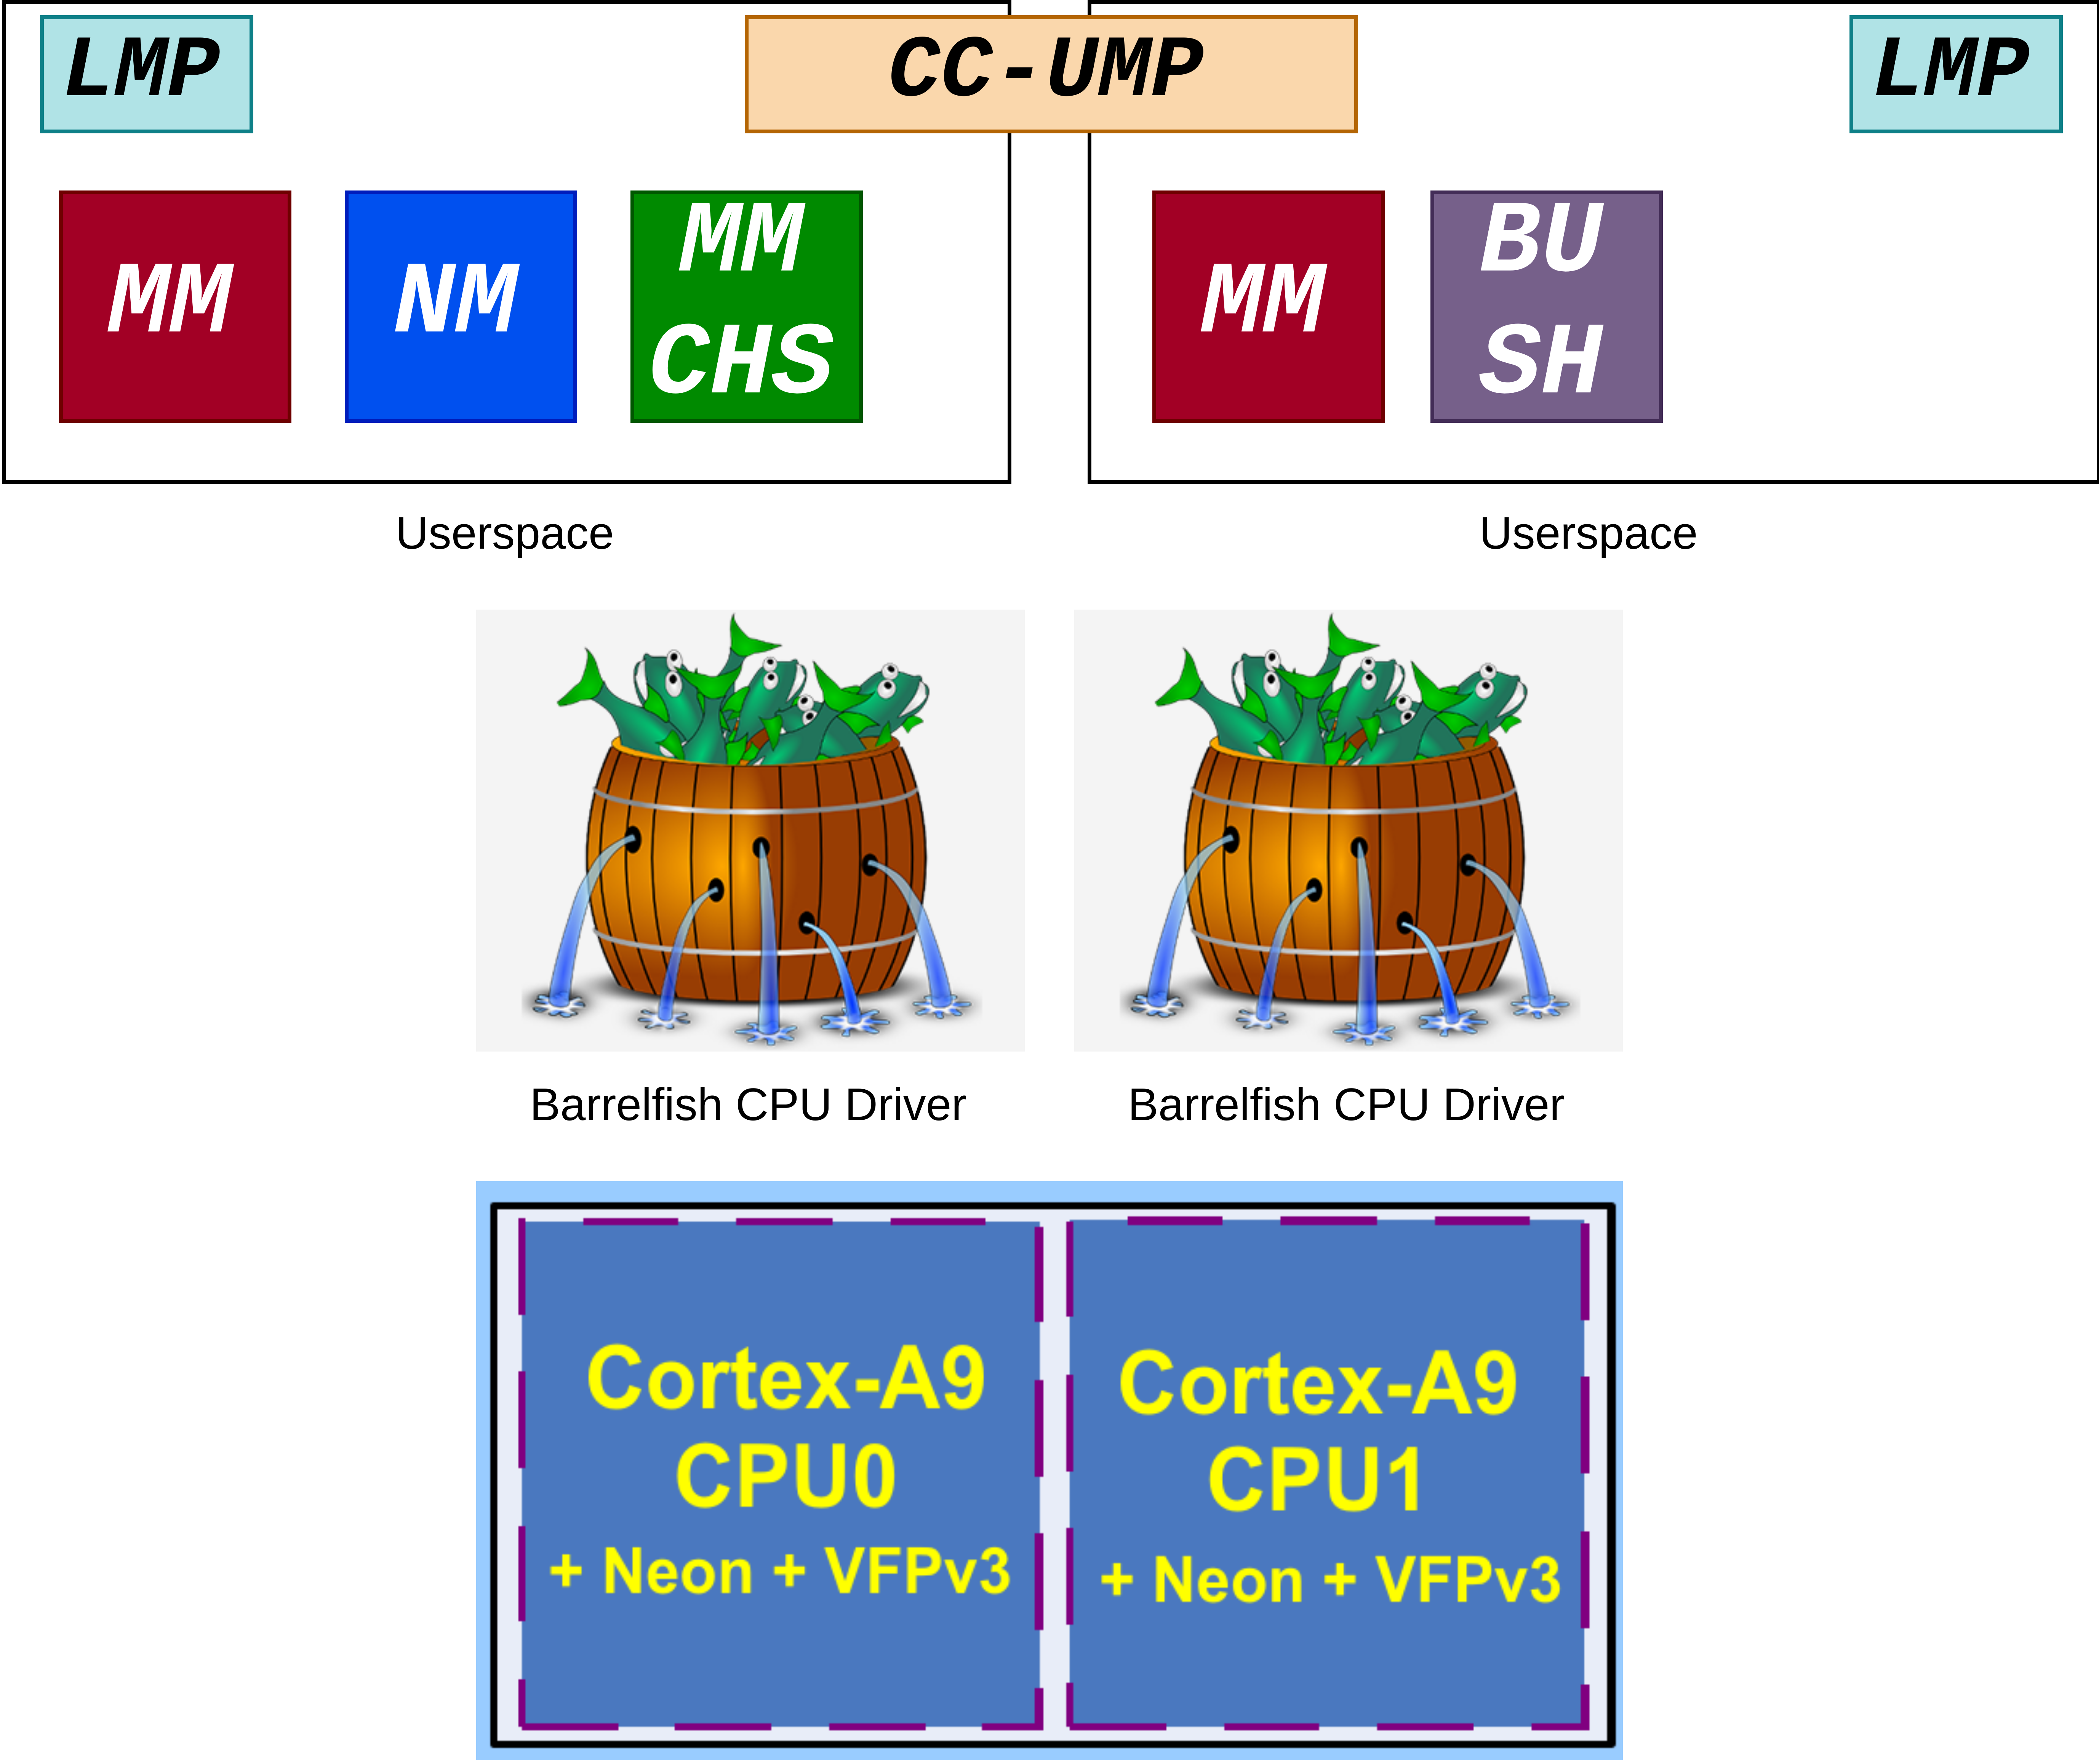
\includegraphics[width=0.8\linewidth]{assets/barrelfish}
	\caption{Components of the implemented system}
	\label{fig:barrelfish}
\end{figure}

The diagram \ref{fig:barrelfish} shows the main components of the implemented system at a very high level.
The project was developed on an OMAP SWPU235ab board - the PandaBoard \cite{panda}. We only booted and used the two main A9 ARM cpus - each core runs a separate instance of the barrelfish kernel.

In userspace, several dispatchers are running:
\begin{itemize}
	\item \textbf{init}, implementing the monitor, and providing the functionalities for the Memory Manager (\textbf{MM}), a Inter-Process Communication (\textbf{LMP}) and the Cross-Core Bridge for IPC (\textbf{CC-LMP});
	\item {mmchs}, implementing the SD card driver (\textbf{MMCHS});
	\item {nm}, implementing the network stack (\textbf{NM});
	\item {bush}, implementing a terminal (\textbf{BUSH})
\end{itemize}

Separating the various components in the init dispatcher would have been possible (and maybe advisable), but was postponed due to time constraints.
The FAT32 file system is implemented as a library.

\newpage
\section{About Our Group}
\textbf{Team K} is comprised of Luca Di Bartolomeo, Matteo Scarlata and Andrea Tulimero. We come from different backgrounds, but we share a passion for information security and working night shifts.

\section{Methods of development}
This project required from the start rapid, evolutionary development, with constant deadlines. The requirements (exception made for this report itself) were stable, but a scarce previous experience of our team in the problem domain meant changes in the understanding of various constraints were possible.

Taking that into account, the obvious software paradigm of choice was an Agile process \cite{agile}. 
We decided to instance a Scum Framework.

\subsection{Scum roles}
The Book and AoS TAs acted as "Product owner", the main stockholders of the product.
The development team consisted in the three of us, alternatively working in extreme programming (XP) pairs.
Matteo covered the role of the Scum Master, coaching the team with Scum principles and setting up the coordination needed for the Scum Workflow.

\begin{figure}
	\centering
	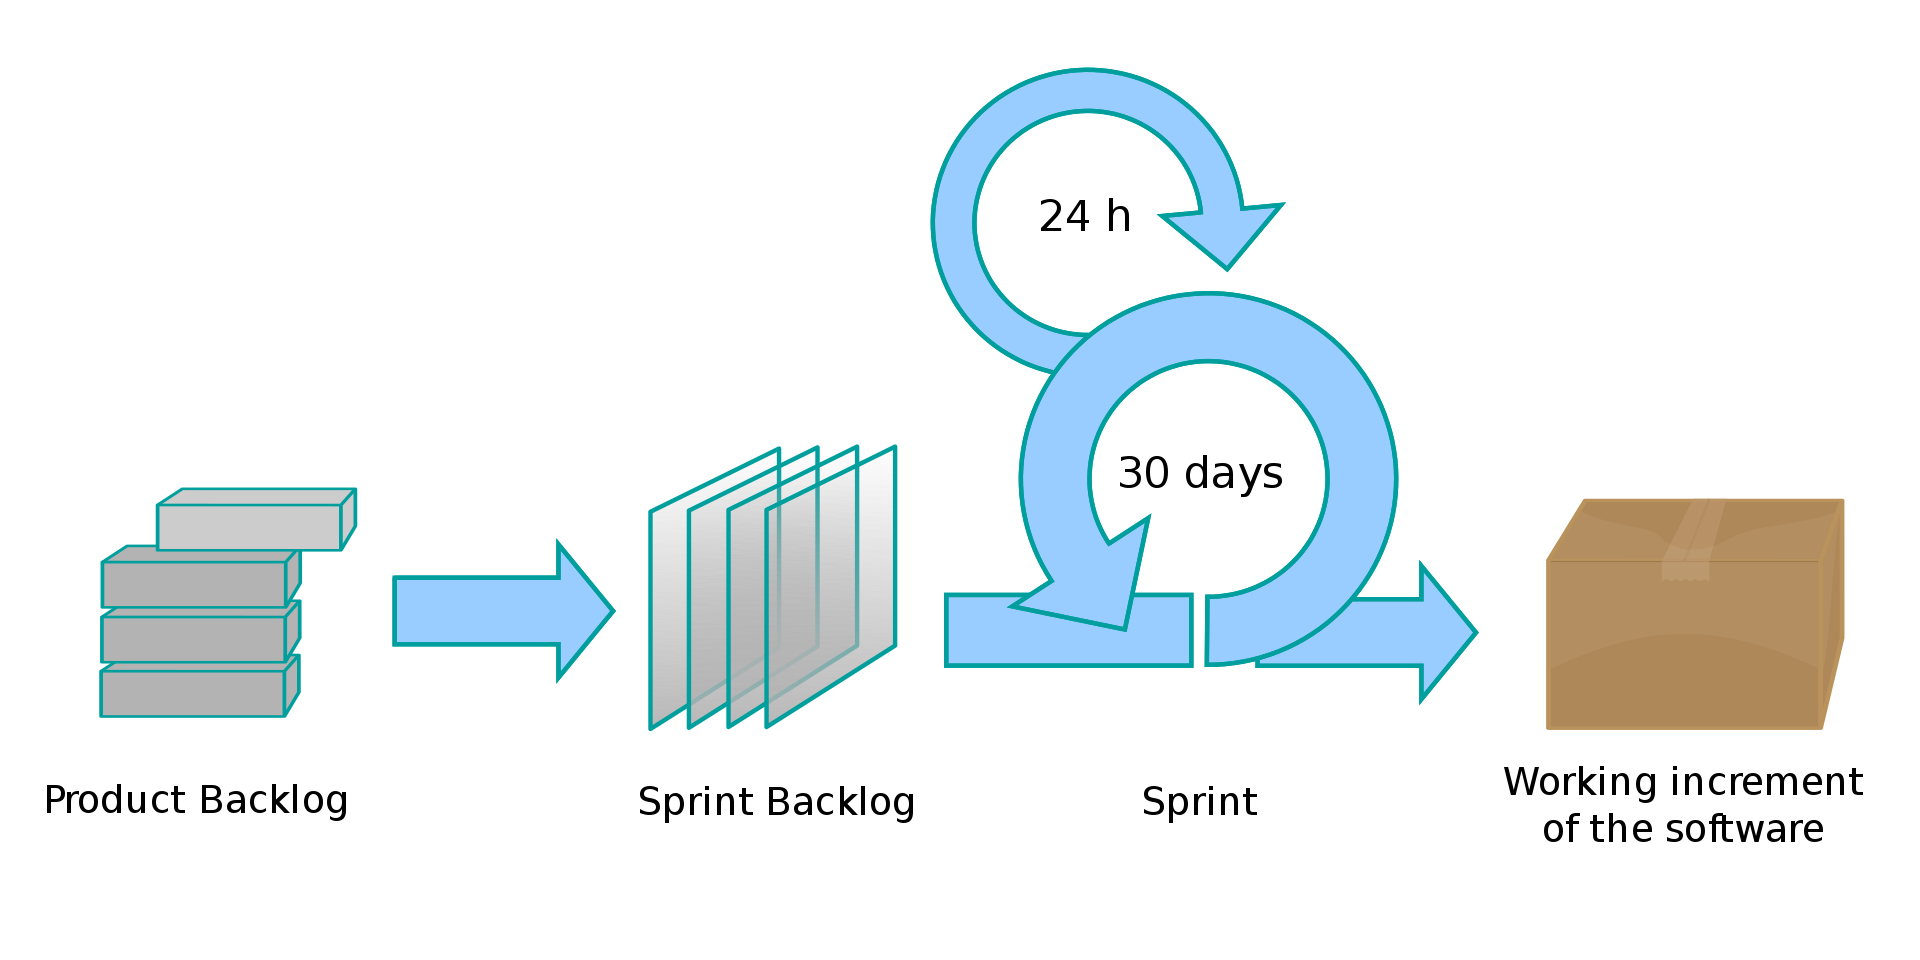
\includegraphics[width=0.7\linewidth]{assets/scrum}

	\caption[The Scum Process]{The Scum Process \cite{scum}}
	\label{fig:scrum}
\end{figure}

\subsection{Scum process}

\textit{Sprints} constituted the basic unit of development. Each Sprint was planned to be one week long - perfectly fitting the course's weekly deadlines. 

A \textit{Sprint Planning} event was held at the start of each spring - defining the sprint backlog to be all the milestone's objectives, including the Extra Challenges. Before the planning meeting, each developer read the full milestone text and any eventual additional background material. During the planning meeting, general decisions regarding the architecture of the part of the OS being implemented were taken. A concrete work plans was elaborated and assigned to each developer.

\textit{Daily Scrums} in the computer labs were held, usually before the start of the daily sprint. In the Scum spirit, those scums were open - and usually included random members of other AoS teams fortuitously working in the same room. Blocking issues and relative workarounds were discussed.

At the conclusion of each spring, the milestone assessment by the AoS Team acted as a \textit{Sprint Review}: an external (and more neutral) look at our work gave us precious feedback, and directed us on the focus points for the successive sprint.

Finally, after the review a brief \textit{Sprint Retrospective} session was held between the team members, to have a final balance of the week.

\section{Prior work and acknowledgments}
The structure of this report has been inspired by the SEL4 Reference Manual \cite{sel4}.

Design choices at various points in the project follow the example of notable OSs in circulation. Particularly, Linux has been a precious reference for us: given its popularity it was easier to find didactic material about its implementation internals, and our team had previous experience with its codebase. FreeBDS, with its clean and extremely well-documented code, has been a good reference implementation of the network stack.


\chapter{Kernel Services and Objects}
Barrelfish provides an extremely limited number of kernel primitives, offloading most of the traditional services implementation to the userspace.
This includes memory allocation, threading and 
\begin{figure}
	\centering
	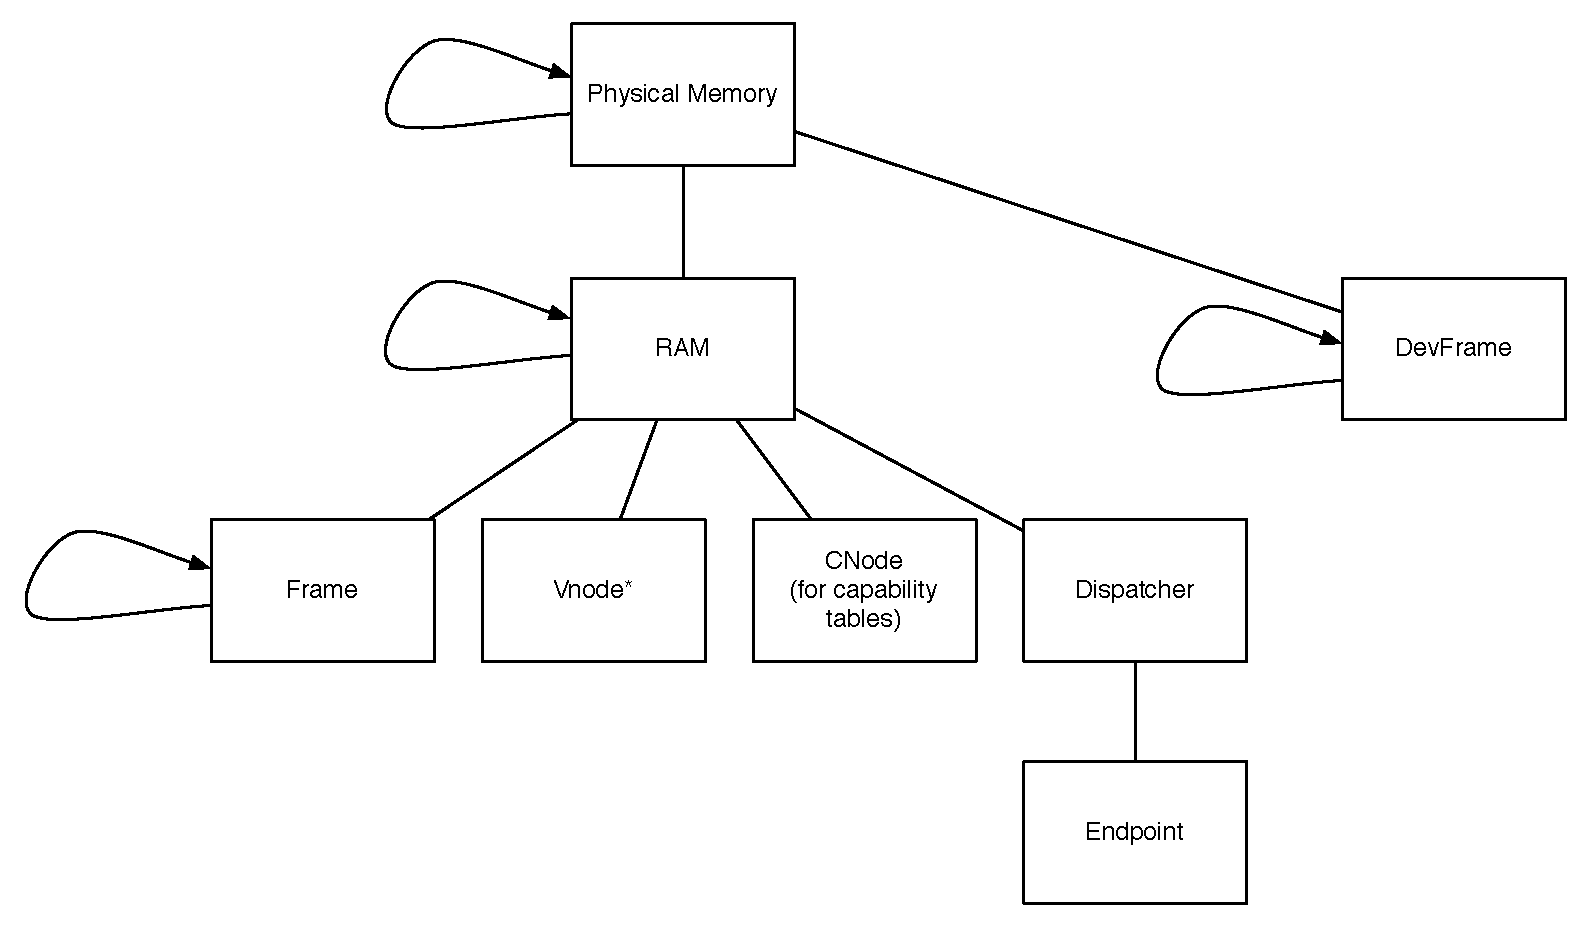
\includegraphics[width=0.7\linewidth]{assets/cap_heirarchy}
	\caption{}
	\label{fig:capheirarchy}
\end{figure}
\begin{figure}
	\centering
	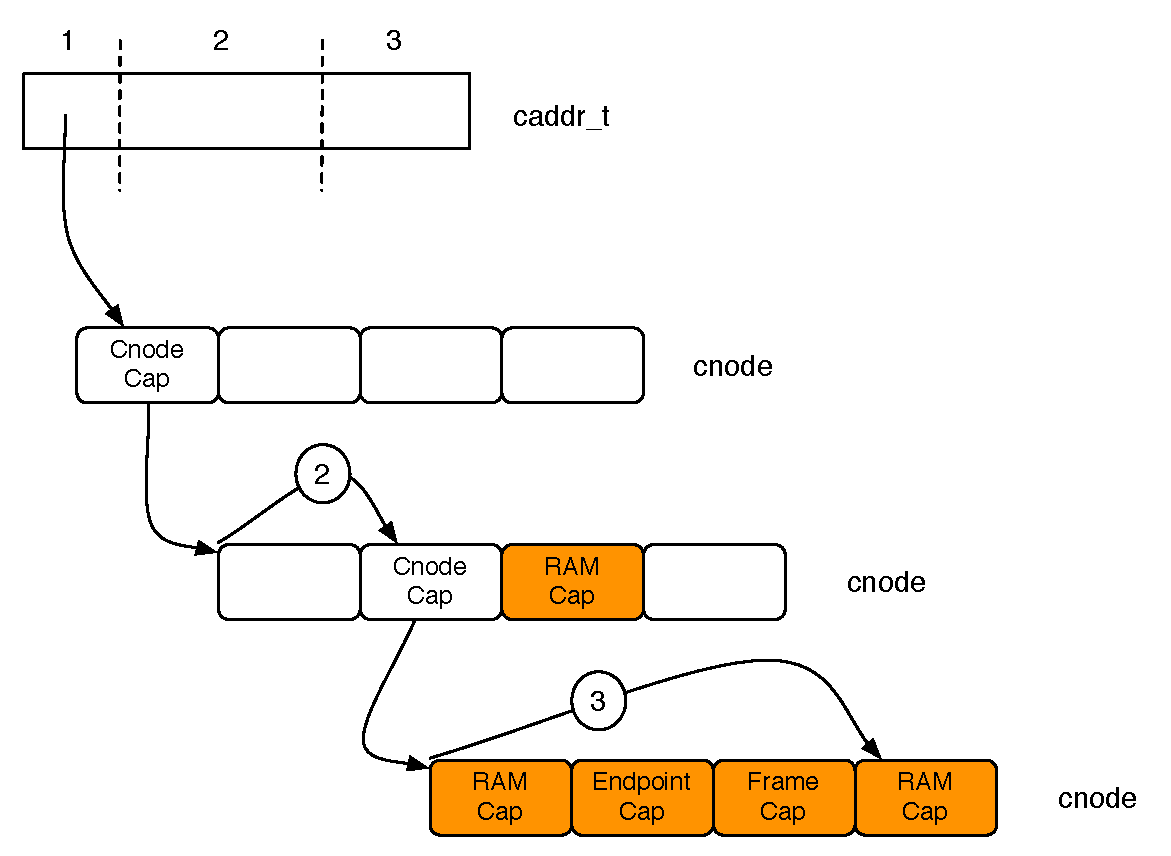
\includegraphics[width=0.7\linewidth]{assets/cap_translation}
	\caption{}
	\label{fig:captranslation}
\end{figure}

\section{Capabilities}
\section{Capability Invocation}
\section{Kernel Memory Allocation}

\chapter{Memory Management}
MILESTONE 1
\section{Physical Memory}
\subsection{Overview}
The memory manager is arguably one of the key parts in the design of an operating system.
Its role, consists of assigning chunks of physical memory (often called pages) to processes requesting for it.

Unlike many other operating systems, in Barrelfish, the communication between the \emph{memory manager} and a process requesting memory does not happen directly through some kind of \emph{system call}.\\
In fact, the whole process is mediated by a \emph{memory server}\footnote{A server is a process that, offers a service to other processes running in the operating system}, which in our case is the \emph{init} process, and the communication amongst the client process and the memory server is carried out through RPC (see Chapter \ref{cap:message_passing}).

The memory is managed thought capabilities - the monitor is given by the kernel RAM capabilities to the full memory space. Those capabilities are managed by our memory manager, who provides them to the other components of the operating system who require them, splitting big chunks in smaller ones and keeping track of which ones are allocated and free.

The capability system introduces additional complexity in the memory management - due to some internal kernel bookkeeping constraints, two RAM capabilities cannot be merged together easily. In particular:
\begin{itemize}
	\item the parent capability must be kept when splitting it,
	\item when all of the children capabilities are destroyed, the parent can be used again freely, but:
	\item if the children capability are only partially destroyed, the rightmost capability needs to be destroyed before other capabilities can be created from the parent.
\end{itemize}

This ruled out many of the simpler memory management architectures, and made fragmentation prevention harder.

\subsection{Fixed-size memory chunks}
As mentioned, the memory manager plays a key role inside an operating system, thus, we decided to make it simple, solid and, last but not least, fast.

We decided never to destroy capabilities, and we took inspiration from Linux\cite{iperf3}, in which memory chunks are divided into categories according to their size, which is fixed.
Each chunk belongs to a bucket, in which all chunks of the same size are kept.\\

This, means that when a process requests a memory chunk to the memory manager, the latter gives back to the former a memory chunk whose size is greater than or equal to the amount of memory requested, such that the size coincide with the nearest \texttt{BUCKET\_SIZE} large enough to accommodate the request.

On the other hand, when a chunk of memory is released, that chunk is not destroyed, but instead it is inserted into a bucket of free chunks, all with the same size.

This approach makes the process of assigning memory chunks, extremely trivial and tremendously fast, in case there is already a free chunk compatible with what requested.
Moreover, it allowed us to bypass some limitations of how the ram capabilities 

\subsection{Alternative design: The buddy system}
After implementing the fixed-size buckets approach we describe in the previous section, we finally found a somewhat nicer data structure: the buddy system. This strategy, too, comes from the Linux world.

In the buddy system the memory manager maintains several buckets, with all the power of two sizes. If a memory if size n is requested the original memory chunks are splitted until a chuck of the next nearest power of two is produced. Every time a chunk is split in two, both halves are inserted in the corresponding bucket, each containing a pointer to the other.

This would have allowed to easily keep track of which ram capabilities can be merged, while maintaining optimal complexity bounds on both the allocation and the free.

Sadly, we did not have time to go back to the memory manager, and the one we implemented was good enough.

\subsection{Choosing the \texttt{BUCKET\_SIZE}}
The different sizes of \emph{buckets} that can be found in the memory manager, are dictated by the ARMv7 specification itself.

In fact, as stated in ARMv7 Specification\cite{arm_docs}, the entries that can be stored in the TLB are the following:
\begin{itemize}
    \item \textbf{Small pages}: 4KB blocks of memory ($2^{12}$ bits)
    \item \textbf{Large pages}: 64KB blocks of memory ($2^{16}$ bits)
    \item \textbf{Sections}: 1MB blocks of memory ($2^{20}$ bits)
    \item \textbf{Supersections}: 16MB blocks of memory ($2^{24}$ bits)
\end{itemize}
Working with memory chunks (in the specification referred as \textit{pages}) with a size incompatible with the entries that can be accommodated in the TLB, would mean losing the speed improvement brought about by the usage of the TLB.

Hence, we opted for having each \texttt{BUCKET\_SIZE} coincide with one of the aforementioned pages' sizes.

\subsection{Unaligned memory requests}
For the sake of simplicity, we are going to analyze first the case in which the requested memory chunks needs not to be aligned in memory.

% TODO: Insert a reference to barrelfish RAM_Type
First of all, it is important to notice that in Barrelfish, in order to work with memory\footnote{In this section when we talk about memory we refer to the RAM\_Type memory of Barrelfish}, and to distribute it, we need to have a capability.
When it is first started, the memory manager, receives (by the init process) some capabilities for all the physical memory that can be used by the system, and we store this capability in a \texttt{dlinked\_list} of \texttt{masters}\footnote{\texttt{dlinked\_list} is a library developed by us which offers primitives to work with double-linked lists}.

Once we have this capability, we can then distribute memory chunks. This process, consists of  \emph{retyping} our master capability in two smaller capabilities, one that will be related to the requested chunk, and another which will be related to the memory not yet allocated to anyone.

As we said previously, when a chunk if freed it is not destroyed, but rather inserted into a bucket of free chunks.
This, means that if there is a free chunk of the same size (after making a round-up) as the requested memory, we can just pick it with a head-removal from the \texttt{dlinked\_list} of free nodes of the according \texttt{BUCKET\_SIZE}, which takes just $\bigO(1)$.

In case there is no free chunk able to accommodate the request, gathering a free chunk takes $\bigO(C)$, where $C$ is the number of master capabilities (which is in the order of ten masters, so it is still pseudo-constant). The steps involved are the following:
\begin{pandacode}
/**
 * Create and return a new suitable node from the masters node
 */
errval_t mm_alloc_from_master(
  struct mm *mm, 
  size_t size,
  size_t alignment,
  struct capref *retcap,
  struct mmnode** node_p) {
  /**
   * If we cannot find a suitable node amongst the free ones
   * in the buckets, we look inside one of the free masters
   */
  errval_t err;
  size = page_round_up(size);
  struct mmnode* master = (struct mmnode*) dlist_head(&mm->masters_dlist);
  while (master) {
      /**
       * If `node->base` is aligned to `alignment` we check that:
       * - The node->size is >= than the requested size
       */
      if ((master->base + master->cap.base) % alignment == 0 &&
        master->size >= size) {
        struct capref node_cap;
        if (err_is_fail(alloc_slot(mm, 1, &node_cap))) {
            return MM_ERR_SLOT_NOSLOTS;
        }
        err = cap_retype(
            node_cap, 
            master->cap.cap, 
            master->base, 
            mm->objtype, 
            size, 1);
        DBGERR(err, "failed cap retype");
        master->base += size;
        master->size -= size;
        *node_p = slab_alloc(&mm->slabs);
        struct mmnode* node = *node_p;
        if (node == NULL) {
            DEBUG_ERR(MM_ERR_SLOT_NOSLOTS, 
                "Node null when requesting slab");
            return MM_ERR_SLOT_NOSLOTS;
        }
        node->type = NodeType_Allocated;
        node->cap.cap= node_cap;
        node->prev = node->next = NULL;
        node->base = master->cap.base + master->base - size;
        node->cap.base = node->base;
        node->size = node->cap.size = size;
        node->bucket = bucket_type(size);
        return SYS_ERR_OK;
      }
      ... // Here the unaligned case is handled
      } else {
          master = master->next;
      }
  }
  return MM_ERR_NOT_FOUND;
}
\end{pandacode}

\subsection{Aligned memory requests}
When dealing with aligned memory requests the situation gets a little bit more complicated, although not excessive thanks to our simple design.
Please note, that all the setup mentioned in the previous subsection still holds for this.

As we mentioned previously, first of all we look for a suitable free chunk in the bucket of free chunks of the according size. This process, takes $\bigO(N/B)$\footnote{Pleas note that the big O notation, ($\bigO$), refers to the worst case scenario}, where $N$ is the amount of memory assigned to out memory manager, and $B$ is the bucket size relative to the requested chunk of memory.
To pick the suitable chunk we just issue a removal from the double-linked list, which takes $\bigO(1)$, so it does not affect the overall asymptotic cost.\\

On the other hand, if we cannot find a node among the free ones, we have to craft a new one starting from a master node. Again, this is not as trivial as the unaligned case.

\paragraph{Reducing to the unaligned case}
The way we decide to solve the requests for aligned memory requests, is by reducing the problem to the simpler unaligned case, and to achieve this, first of all we \textit{massage} a suitable master capability, making it compatible to accommodate the received request.

We do this by first, finding a suitable master capability, such that we have enough space to accommodate the client's request, and to generate some \emph{padding} chunks out of it, which move the master capability base address to be aligned with the request. This padding chunks will be directly inserted in the respective bucket of free chunks.

To better understand what we explained so far, we listed the code in charge of carrying out this procedure below:

\begin{pandacode}
/**
 * Create and return a new suitable node from the masters node
 */
errval_t mm_alloc_from_master(
    struct mm *mm, 
    size_t size,
    size_t alignment,
    struct capref *retcap,
    struct mmnode** node_p) {
  ...
  /**
   * If `node->base` is not aligned to `alignment` we check that:
   * - The node->size is >= than the sum of:
   *   -- Requested `size`
   *   -- ROUND_UP(node->base, alignment) - node->base
   */
  else if (
      (master->base + master->cap.base) % alignment != 0 &&
      master->size >= 
          (ROUND_UP(master->base + master->cap.base, alignment) 
          - master->base - master->cap.base) + size
      ) {
      size_t pad = ROUND_UP(master->base + master->cap.base, alignment) 
          - master->cap.base - master->base;
      while(pad > 0) {
        size_t pag_size;
        if (pad >= 64*KB) pag_size = 64*KB;
        else pag_size = 4*KB;
  
        struct capref pad_cap;
        if (err_is_fail(alloc_slot(mm, 1, &pad_cap))) {
            return MM_ERR_SLOT_NOSLOTS;
        }
        err = cap_retype(
            pad_cap,
            master->cap.cap,
            master->base,
            mm->objtype, pag_size, 1);
        master->base += pag_size;
        master->size -= pag_size;
        struct mmnode* pad_node = slab_alloc(&mm->slabs);
        if (pad_node == NULL) {
            DEBUG_ERR(MM_ERR_SLOT_NOSLOTS, "Node null");
            return MM_ERR_SLOT_NOSLOTS;
        }
        pad_node->type = NodeType_Free;
        pad_node->cap.cap = pad_cap;
        pad_node->base =  master->cap.base + master->base - pag_size;
        pad_node->cap.base = pad_node->base;
        pad_node->size = pad_node->cap.size = pag_size;
        pad_node->bucket = bucket_type(pag_size);
        // Insert the free node in the according bucket
        dlist_head_insert(&mm->free_buckets[pad_node->bucket], pad_node);
        // Update the master
        pad -= pag_size;
      }
      continue;
  }
  ...
}
\end{pandacode}
Analyzing this procedure in term of asymptotic cost tends to be a little bit tricky, since it depends a lot on the system configuration.
% In our case, we can assert that alignments over 1 Megabytes are so rare that we can consider the biggest alignment that can be requested is 1 Megabytes.

We can see that the whole procedure takes $\bigO(P/64 + REM(P/64) / 4)$, where $P$ is the number of bytes (in Kilobytes) of padding (which cannot be greater than 1020 Kb, for obvious reasons, since the smallest chunk is 4 Kilobytes), while $64$ and $4$, are the bytesize (in Kilobytes) of the chunks that are used to fill the padding needed for the alignment.


The reason of this approach to deal with unaligned memory requests, arise from the will of avoiding any sort of \emph{hole} in the master capabilities, which would have brought about the need of introducing new data structures to keep track of the chunks of memory inside a master capability that was skipped to accommodate an aligned request.

Instead, we just wanted to have a cursor which points to the first bit of memory which, from that on, is still free.
This, ensures that accessing this free memory is carried out always in $\bigO(1)$, and, since most of the times the memory manager receives requests of unaligned memory requests, the process always takes $\bigO(1)$, whether it is needed to create a new chunk of memory or we can reuse a previously allocated one.


\emph{Virtual memory management and on-demand memory will be discussed accurately in the following chapter.}


\section{Virtual Memory and Paging}

\subsection{Initial paging implementation (Milestone 1)}

After we had a small working version of \texttt{mm.c}, we needed to implement a stub of 
the \texttt{paging\_map\_fixed\_attr()} function.

At first, our function needed to handle only requests smaller than \texttt{BASE\_PAGE\_SIZE}, 
and we also had the guarantee that addresses were page aligned. We implemented a simple wrapper
around the \t{vnode\_map} syscall, and a few simple tests to check that were executed each run to ensure nothing would break without us realizing:


\begin{pandacode} 
void paging_test(struct mm* mm) {
	lvaddr_t vaddr = 0x22ff000;
	struct capref frame;
	size_t bytes = 0x1000;
	int flags = VREGION_FLAGS_READ_WRITE;

	frame_alloc(&frame, bytes, NULL);
	paging_map_fixed_attr(NULL, vaddr, frame, bytes, flags);

	*(lvaddr_t *) vaddr = 0x1337;
	assert(*(lvaddr_t *) vaddr == 0x1337);
}
\end{pandacode}

This test simply wrote a value in a specific address in memory; then made sure that value
was the same when reading from the same address.

\subsection{Paging improvements (Milestone 2)}

For this milestone there was the requirement that \t{paging\_map\_fixed\_attr()} worked with frames of arbitrary size, and could be called multiple times without crashing. 
We needed to keep track of the state of the virtual space, and so we extended the struct \t{paging\_state} in the following way:

\begin{pandacode}
struct pglist {
	bool pg_offset_l2[ARM_L2_MAX_ENTRIES];
};

struct paging_state {
	struct slot_allocator* slot_alloc;
	struct capref l2_caps[ARM_L1_MAX_ENTRIES];
	bool l2_mapped[ARM_L1_MAX_ENTRIES];

	struct slab_allocator pglist_alloc;
	struct pglist* pg_offset_l1[ARM_L1_MAX_ENTRIES];
};
\end{pandacode}

The array \t{l2\_mapped} keeps track of which L2 pages are already mapped or not. 
The \t{l2\_caps} array keeps track of the capabilities used to map L2 pages to the L1 page, 
since we need to reuse them during calls to \t{vnode\_map}. 

We also needed to know beforehand if a certain virtual address was already
mapped or not. We used an array of boolean values for every L2 page,
\t{pg\_offset\_l2}. Every entry of this array represented a 4 KB page in
memory. Every L2 page has 256 possible entries, and the L1 page supports up to
2048 L2 pages mapped; in total, our \t{paging\_state} struct had an array of
524,288 boolean values, which put a considerable weight on memory. We didn't
realize how much of a problem this was until we spent many hours hunting a bug
caused by the fact that we had smashed the stack by allocating one struct
\t{paging\_state} on it.


\subsubsection{Paging\_alloc}

This milestone required us to implement the \t{paging\_alloc} function to be able to look
for a free place in memory to map a frame to when calling \t{paging\_map\_frame\_attr}.

Our first approach consisted in looking if there was a continuous segment of free pages
in the boolean array \t{pg\_offset\_l2} contained inside the struct \t{paging\_state}, by
traversing it from the start until we find a good enough spot.

We also wrote additional tests for the paging functionality, this time by mapping very large 
pages or by mapping thousands of time a single page, such as this:

\begin{pandacode}
void consecutive_pages_big(struct mm* mm) {
	const uint32_t PAGE_NO = 50;
	size_t bytes = 0x1000 * 0x100; // 1 MB
	struct capref frame_m;
	struct capref * frame;

	// make space for "frame" array
	frame_alloc(&frame_m, PAGE_NO*sizeof(struct capref), NULL);
	paging_map_frame_attr(st, (void *) &frame, PAGE_NO*sizeof(struct capref), frame_m, rw_flags, NULL, NULL);

	for (int i = 0; i < PAGE_NO; i++) {
		frame_alloc(&frame[i], bytes, NULL);
		paging_map_frame_attr(st, &buf[i], bytes, frame[i], rw_flags, NULL, NULL);
	}
}
\end{pandacode}

Those kinds of tests not only helped us spot many nefarious bugs, but they also showed us 
how \emph{slow} our implementation was. In fact, running the above test took tens of seconds
to complete, which is really too much time to just map 50 MB of memory.
After realizing that almost all of the time was spent inside \t{paging\_alloc} looking
for a good enough spot in the virtual space, we decided to rewrite how the \t{paging\_state}
kept track of which pages are mapped to make this kind of search faster.

We came up with the idea of using a double-linked list of "chunks", where each chunk represented
an occupied segment of virtual space, defined by the \t{base} and \t{end} pointers:

\begin{pandacode}
struct pgchunk {
	struct pgchunk *prev;
	struct pgchunk *next;
	lvaddr_t base;       
	lvaddr_t end;        
};
\end{pandacode}

The reasoning behind this was that if we managed to keep this list \textbf{sorted}, and managed to implement
a smart \textbf{merging} strategy between chunks (e.g. if there are two consecutive chunks,
they can be replaced by one single big chunk that spans over the memory defined by the previous two), 
we would have had a list that contained not many elements and that could be traversed only once to find
a free spot in memory. In addition, we also decided to modify the \t{paging\_alloc} algorithm such that
it would favour returning pages adjacent to already occupied pages so that we could maximize the amount
of chunks merged.

This approach turned out to be rather complex, we had particular trouble
implementing \t{paging\_unmap()} (unmapping a page in the middle of a chunk
required a split of that chunk into two, keeping the list sorted), and we also
found not so easy avoiding recursive calls into \t{paging\_map\_fixed\_attr()}
(New chunks were allocated through \t{slab\_alloc()}; if the slab allocator ran
out of slabs while being inside \t{paging\_map\_fixed\_attr()} it would call
itself again to allocate memory - more on how we solved this later), but after
some time we had a working solution that passed all tests. You can find the 
implementation of this new approach in functions \t{mark\_chunk\_used()}, 
\t{mark\_chunk\_free()} and \t{paging\_alloc()} in file \t{lib/aos/paging.c}.

It was a lot of effort but also very rewarding: our tests showed that the merging
strategy worked very well, as the linked list of chunks rarely exceeded 3-4 elements.
In addition, all tests that before took considerable time now were completed in under
a second.


\subsubsection{Fixing the slab refilling}

As previously mentioned, we had a curious bug in which we noticed that
\t{paging\_map\_frame\_attr()} was calling itself recursively, and causing a
kernel panic due to trying to map twice the same page.  In particular, the bug
showed up only after we did a great number of page mappings/unmappings, and it
was seemingly random.  In the end, we found out that the cause was the slab
allocator running out of slab space while trying to allocate new space for a
new chunk while marking some memory as occupied inside
\t{paging\_map\_fixed\_attr()}.  The \t{slab\_alloc()} function called
\t{slab\_default\_refill()}, which in turn called
\t{paging\_map\_frame\_attr()} to refill the slab space. When being called the
second time, the \t{paging\_alloc()} function selected the same free virtual
space that the original \t{paging\_map\_frame\_attr()} selected (because the
space wasn't marked as used, as we didn't have memory to allocate a new chunk
to insert in the double-linked list \t{pgchunk}!). In the end, the two
instances of \t{paging\_map\_frame\_attr()} selected the same page and executed
one after another causing a kernel panic, a classic case of \emph{Time of Check / Time of Use} bug.

We spent a lot of time thinking for an elegant solution to avoid this
behaviour, but then we settled for a simple hack the job done. Since we had the
guarantee that the \t{pgchunk} linked list had always at least one element, 
we extended the \t{end} pointer of the previous chunk in the list to cover all
the virtual space \t{paging\_alloc} selected before asking to allocate a new chunk;
after being done with the allocation, the \t{end} pointer of the previous chunk was
restored with its previous value and the new chunk was added to the list:

\begin{pandacode}
//Example of adding a new chunk at the tail of the pgchunk list
struct pgchunk* tail = (struct pgchunk*) list->tail;
lvaddr_t oldend = tail->end;
tail->end = vaddr + bytes; // mark space as reserved to avoid recursion
struct pgchunk* newchunk = slab_alloc(&st->pgchunk_alloc);
newchunk->base = vaddr;
newchunk->end = vaddr + bytes;
tail->end = oldend; // shrink the previous chunk back to original size
dlist_tail_insert(list, newchunk); // append newchunk to the end of the pgchunk list
\end{pandacode}

In this way, the recursion still happens, but the second call to \t{paging\_alloc()} cannot
select the same virtual space as the first call because it sees that the "previous" chunk 
covers it completely.




\subsection{On-demand memory (Milestone 4)}

\subsubsection{Page fault handling}

Our pagefault handler is the function \t{exception\_handler()} inside file \t{lib/aos/paging.c}
Each process has its own, and it works in userspace. One particular difficulty of designing
the pagefault handler is avoiding causing other pagefaults while handling a pagefault.

As soon as we got a stub of the pagefault handler working, we unset the \t{USE\_STATIC\_HEAP}
flag inside \t{lib/aos/morecore.c}, and used the following implementation of the morecore functions:

\begin{pandacode}
static void *morecore_alloc(size_t bytes, size_t *retbytes)
{
	struct morecore_state* mst = get_morecore_state();
	void* p; 
	paging_region_map(&mst->region, bytes, &p, retbytes);
	return p;
}

errval_t morecore_init(size_t alignment) {
	struct morecore_state* mst = get_morecore_state();
	paging_region_init(
			get_current_paging_state(),
			&mst->region,
			HEAP_REGION_SIZE); // 512 MB
	thread_mutex_init(&mst->mutex);
	sys_morecore_alloc = morecore_alloc;
	sys_morecore_free = morecore_free;
	return SYS_ERR_OK;
}
\end{pandacode}

Basically, every process had 512 MB of heap to work with, as a \emph{reserved}
but still \emph{unmapped} region of virtual space. This meant that a call to
\t{malloc()} could return unmapped memory, that would be mapped by the
pagefault handler as soon as that memory was accessed.

Since the handler must map a page at the faulting address, it needs to have a
fresh \t{frame} that can be mapped at the given address. If the faulting
process is init, then this is not a problem, as a call to \t{frame\_alloc()}
will mean a call to \t{mm\_alloc\_aligned()} which can not trigger pagefaults.
However, if the faulting process is not init, then it poses a problem, as
memory must be asked through an LMP call to init, and our implementation of LMP
inside \t{lib/aos/aos\_rpc.c} \emph{was not} pagefault-safe, as it heavily
relied on the heap through \t{malloc()} calls.

At this point, we had two choices to solve this problem:
\begin{itemize}
	\item Make sure the pagefault handler has always a free \t{frame} that can
		use as soon as the next fault happens, thus avoiding the call to
		\t{frame\_alloc()}.
	\item Rewrite our implementation of LMP inside \t{lib/aos/aos\_rpc.c}, to
		make sure it will never trigger a pagefault.
\end{itemize}

After a bit of discussion, we decided to go with the second option. It was not
the easiest option, but it was the most elegant and helped us a lot later in
Milestone 6 when we merged the interfaces for LMP and UMP. To make the LMP
code pagefault-safe, we used as little memory as possible, and allocated all
variables on the stack. We knew the stack was large enough for our allocations,
because we assigned the stack to the pagefault handler ourselves in function
\t{paging\_init\_onthread()} (more on this later).

To check if the \t{malloc()} was working as intended, we did a test in which we
allocated a huge buffer through \t{malloc()} but actually only used four bytes
in the middle of that buffer; since we had a \t{debug\_printf()} in the
exception handler, we could see with our own eyes how many pages of that buffer
were actually allocated. The code for the test is the following:
\begin{pandacode}
static void huge_malloc(struct mm* mm) {
	size_t bytes = 0x100000 * 100; // 100 MB
	int *c = malloc(bytes);

	*(c + bytes/8) = 0xcafebabe;
	assert(*(c + bytes/8) == 0xcafebabe);
	free(c);
}
\end{pandacode}
The test was successful, as the pagefault handler was called only once (only a
single page was mapped, instead of the entire buffer).


\subsubsection{Handling pagefaults for more than one thread}
If a process can have multiple threads, they can pagefault at the same time. To
avoid multiple instances of the pagefault handler stepping on each other's
stack, we thought
about two choices:
\begin{itemize}
	\item Make sure every thread has a different stack for its own pagefault
		handler. In this way, multiple instances of the handler can run
		interleaved without any problems.
	\item Enforce the presence of a single pagefault handler that solves
		pagefaults to all threads on demand, waiting on an event loop with a
		queue for incoming pagefaults.
\end{itemize}
Although the second choice was more elegant, in the end we went for the first
one, mostly for lack of time. This is the code for
\t{paging\_init\_onthread()}, which makes sure that each thread has a different
stack for its exception handler:
\begin{pandacode}
void paging_init_onthread(struct thread *t) {
	t->exception_handler = &exception_handler;
	void *stack = calloc(0x10000, 1); // 1 MB
	t->exception_stack = (void*) stack;
	t->exception_stack_top = (void*) stack + 0x10000;
}
\end{pandacode}
As you can see, the stack is allocated with a call to \t{calloc()}. We don't
particularly care that the memory is zeroed out, we use \t{calloc()} to make
sure that all that memory is mapped (because it will be accessed while zeroing
out) to avoid having a pagefault handler triggering a pagefault because of
using its own stack.


\subsubsection{A subtle bug}
During our tests, we noticed that if a process spawned more than 13 threads,
and each of the threads filled up a newly requested buffer through \t{malloc()},
causing numerous pagefaults, as soon as the 14th thread spawned and caused a 
pagefault, our process would crash because of having triggered a pagefault while
handling another one.

After \emph{numerous} hours debugging, we found out that the culprit was the function
\t{lmp\_chan\_alloc\_recv\_slot()}, which called \t{slot\_alloc()}, which
would trigger a pagefault when there were no more slots available for storing
a capability!

We solved this by adding a new parameter to the function
\t{two\_level\_alloc()}, a boolean called \t{should\_refill}, which determined
if the function could consider refilling the slots or not. When called inside
\t{lmp\_chan\_alloc\_recv\_slot()}, the boolean was always false, meaning that
no more nested pagefaults would be triggered.  However, we also increasing the
treshold for when the slots are refilled up to 8, so that there are a few slots
that can be used when \t{should\_refill} is false.

The positive thing is that solving this bug made us complete the extra challenge
relative to running out of capability slots for this milestone, and we only
found out about the extra challenge later.


\subsubsection{Paging thread safety}
In this milestone we also had to make sure that the code inside
\t{lib/aos/paging.c} was thread safe. We use two locks, kept inside the
\t{paging\_state} struct.  The first one is for the function
\t{paging\_map\_frame\_attr()}, and is meant to ensure that two calls to
\t{paging\_map\_frame\_attr()} will not interleave causing the first the
execution of two \t{paging\_alloc()} and then two
\t{paging\_map\_fixed\_attr()}, trying to map the same page of virtual space.
The second lock guards the function \t{paging\_map\_fixed\_attr()}, making sure
that only one thread can execute that function at a time. The lock is obtained
at the very start of the function and is released only at the very end (or in
case of early exits due to errors). We were aware that this \emph{Big Paging
Lock} strategy was not optimal at all: the only piece of shared memory between
threads that needed attention was the \t{paging\_state} struct; we could have
used more fine-grained locks or even implemented atomic read/writes for the
\t{paging\_state}, but we were dangerously running out of time during this
milestone, so we had to settle for the cheap \emph{Big Paging Lock}.

One interesting thing we learned while implementing the \emph{Big Paging Lock}
was to use nested locks (by calling \t{thread\_mutex\_lock\_nested()} instead
of \t{thread\_mutex\_lock()}).  We had to use nested locks because of the fact
that both \t{paging\_map\_fixed\_attr()} and \t{paging\_map\_frame\_attr()}
could happen to call themselves recursively in case of one slab allocator
running out of slabs.

\subsubsection{Paging Regions}

We needed to further modify our paging implementation when we were required to
make self paging work. First of all, we needed to add the concept of paging
regions, reserved regions of virtual space. 

For this reason, we decided to keep another linked list in the
\t{paging\_state} struct, made out of \t{struct pgchunk} elements (See chapter
on Milestone 2 for further details on the \t{pgchunk} struct), which
represented chunks of \emph{reserved memory}.

We decided to enforce the following policy: every process can ask to reserve a
chunk of memory via a call to \t{paging\_region\_init()}; however, only a page
which is in a reserved region can only be mapped by the \emph{page fault
handler}. Moreover, the \t{paging\_map\_frame\_attr()} function will never
attempt to map a page in a reserved region.

While implementing this, one problem quickly arised: the \t{paging\_alloc()}
function, which had the job of finding a free space in the virtual space for a
given mapping, had to go through \textbf{two} different linked lists in order
to find a free and non reserved spot. Implementing this would have been tedious
and error-prone, so after giving it some thought we decided to make the list of
reserved regions a \emph{superset} of the list of occupied regions of virtual
space. This meant that every time a reserved region was requested, the list of
reserved regions would be updated; every time a page was mapped, \textbf{both}
the list of reserved regions and the list of occupied regions would be updated.

Thanks to this, \t{paging\_alloc()} was very easy to modify because now it
required going through only the linked list of reserved regions, because that
contained occupied regions too.

To ensure efficiency with this approach, all the optimizations that were done
in Milestone 2 to the linked list of chunks of occupied pages (merging
consecutive chunks, keeping the list sorted) were done on the linked list of
reserved regions too.

Unfortunately, we didn't have the time to differentiate between different kind
of regions (which one represented the heap, which one the stack, and so on), so
we let the \emph{page fault handler} map every page that was requested inside a
reserved region, without checking if the calling thread had the permissions on
that reserved region or not.


\subsubsection{Extra challenge: dynamically expanding the stack}
To ensure that each thread had a reasonable stack size, but without the need to
map all of the stack when spawning the thread, the function
\t{threads\_create\_unrunnable()} uses \t{malloc()} to allocate the stack for
each thread. The stack will be mapped page by page as soon as it is used by
throwing page faults. However, the pagefault handler checks each time the
\t{sp} register to check if the stack pointer is between the current thread's
\t{stack} and \t{stack\_top} bounds. If the stack pointer is out of bounds, the
pagefault handler will throw a \emph{stack overflow} error and quit the current
thread.

\subsubsection{Extra: bug found in the kernel}
During this milestone, we had a curious bug that caused a buffer overflow,
smashing the stack, overwriting the return address and sending the instruction
pointer in apparently random places of the virtual space. It was particularly
hard to debug this and understand its cause because the kernel crashed with
different errors each time.  While investigating why the errors were different
each time, we actually found another unrelated bug, but this time not in our
code, but inside the kernel.

We noticed something was very wrong when one time we found out that the
instruction pointer of a thread was \emph{inside another thread's stack}.
Instead of crashing because of a segmentation fault (we made sure that the
stack was not mapped as executable), it crashed with something relative to an
execution error. We started to suspect there was something fishy going on with
paging permissions, and tried to map every process' \t{text} section as
non-executable; but every process still ran fine (we should have gotten a crash
as soon as init tried to spawn another process).

After some digging, we found out that there was an error in \t{kernel/arch/armv7/paging.c}
in function \t{paging\_set\_flags}:
\begin{pandacode}
static void
paging_set_flags(union arm_l2_entry *entry, uintptr_t kpi_paging_flags)
{
		entry->small_page.tex = 1; /* Write-allocate. */
		entry->small_page.shareable = 1; /* Coherent. */
		entry->small_page.bufferable = 1;
		entry->small_page.cacheable =
			(kpi_paging_flags & KPI_PAGING_FLAGS_NOCACHE) ? 0 : 1;
		entry->small_page.ap10  =
			(kpi_paging_flags & KPI_PAGING_FLAGS_READ)  ? 2 : 0;
		entry->small_page.ap10 |=
			(kpi_paging_flags & KPI_PAGING_FLAGS_WRITE) ? 3 : 0;
		entry->small_page.ap2 = 0;
		//entry->small_page.type = (kpi_paging_flags & KPI_PAGING_FLAGS_EXECUTE) ?
		//	L2_TYPE_SMALL_PAGE : L2_TYPE_SMALL_PAGE_XN; 
}
\end{pandacode}
The function did not correctly set the \t{NX} bit of the pages, setting all mapped 
pages as executable by default. The commented line is the patch that we sent to the
mailing list that fixes the bug.

\chapter{Units of Execution}
\begin{figure}
	\centering
	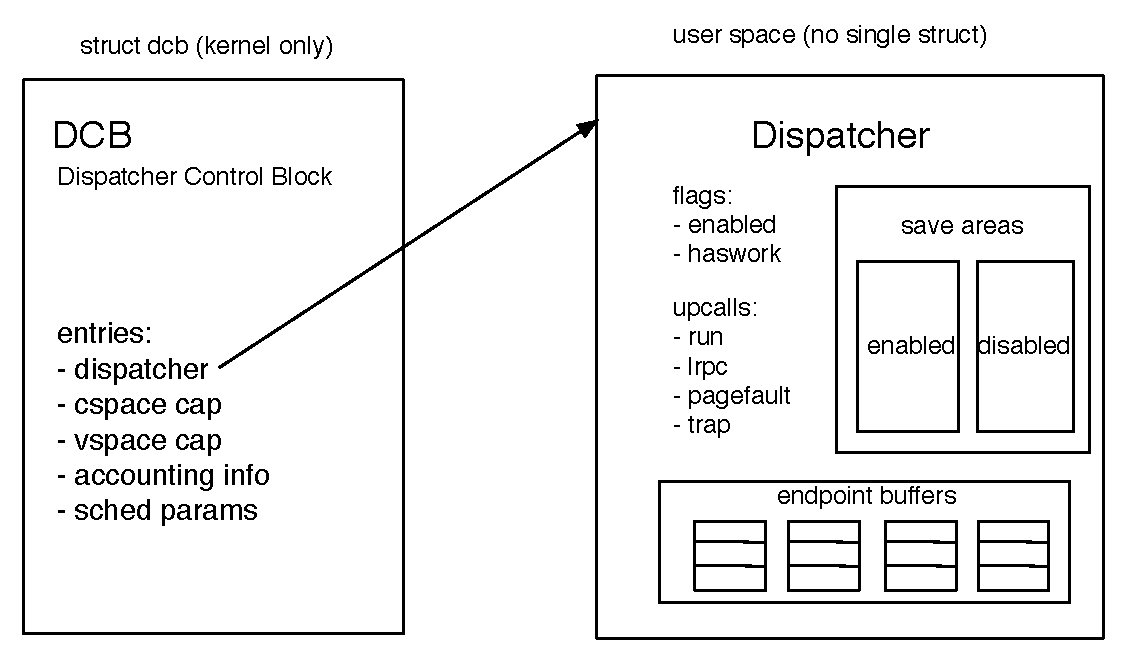
\includegraphics[width=0.7\linewidth]{assets/dcb}
	\caption{The dispatcher Control Block (from: \cite{barrelfishdoc})}
	\label{fig:dcb}
\end{figure}

Barrelfish provides one abstraction for the user processes: the dispatcher. A dispatcher is an independent unit of execution: it has its own capability space and virtual address space. The kernel will only create and run the dispatcher of the monitor process (\texttt{init}), all other dispatchers will be created in user space and made runnable by the kernel.

Coherently with its microkernel design, Barrelfish does not provide kernel threads: threading needs to be implemented in user space.

The following section will describe, in order, the process of spawning a new dispatcher, and the threading model and code.
\section{Dispatchers}
\label{sec:dispatchers}
Most commonly known as processes -- in other popular operating systems such as Unix or Windows -- the dispatchers are the basis of user-level programs running in Barrelfish.
And being a microkernel, lots of basic services -- such as memory management -- are offered by user-level programs.

On a high level, the steps involved in the spawn of a process are quite similar among different operating systems, although, due to the different nature of operating systems, some of these steps might be profoundly different (such as the lack of the \texttt{fork()} in Barrelfish).

Some peculiarities in the spawning of a dispatcher in Barrelfish, are also brought by the fact that the \emph{CPU driver} is stateless, hence all the data structures -- or at least almost all of them -- are provided to it by user-level programs.
This, means that if we want to spawn a process from another one, we need to provide the CPU driver with all that is needed to spawn the new instance of the target program.

Furthermore, since in Barrelfish we have capabilities, we need to setup not only the VSpace (Virtual Space) of the process we are spawning, but also the CSpace (Capability Space) -- which is much like a Virtual Space equivalent for capabilities.

In the next subsections we are going to break down and thoroughly analyze the different steps involved in the spawning of a dispatcher in Barrelfish.

\subsection{Loading the ELF in memory}
First things first, we need to load the program to spawn in memory. Currently, the only executable type supported from our system is the \emph{ELF} (Executable and Linkable Format), which is the executable file type found in most Unix-like systems.

We can load the program from two sources:
\begin{itemize}
    \item \textbf{Filesystem}: thus from a storage device, which in our case is an SD card
    \item \textbf{Multiboot}: which is embedded in the \texttt{bootinfo} at compile time, and is passed to \emph{init} at startup time
\end{itemize}
We will analyze the former method in the section dedicated to the Filesystem, so we will now cover the variant with the ELF loading from the Multiboot image.

In order to map an ELF in memory from the multiboot image, we first need to obtain the region of memory corresponding to the target program. We can do this with the following:
\begin{pandacode}
    // - Get the binary from multiboot image
    struct mem_region * mb;
    mb = multiboot_find_module(bi, binary_name);
    if (!mb) {
        return SPAWN_ERR_LOAD;
    }
\end{pandacode}
Once we have this, the next step is to map the \texttt{mem\_region} in our virtual space.
First, we need to create a \texttt{capref} pointing to the slot holding the capability for that memory region:
\begin{pandacode}
    struct capref child_frame = {
        .cnode = cnode_module,
        .slot = mb->mrmod_slot,
    };
\end{pandacode}
Then, we can map the memory region in our virtual space with:
\begin{pandacode}
    // - Map multiboot module in your address space
    elf_size = mb->mrmod_size;
    err = paging_map_frame_attr(get_current_paging_state(),
    (void**) &elf_file, elf_size, child_frame,
    VREGION_FLAGS_READ, NULL, NULL);
    if (err_is_fail(err)) {
        return err;
    }
\end{pandacode}
Once we have the ELF loaded in memory, we can go on with next phase, that is setting up the CSpace

\subsection{Setting up the Capability Space}
\label{sub:setting_up_cspace}
In this create an initial CSpace layout for the spawned dispatcher.
First of all, we need to create an L1 Cnode which is to be the root Cnode of the dispatcher:
\begin{pandacode}
    // - Create root CNode
    err = cnode_create_l1(&si->croot_cap, &si->rootcnode);
    DBGERR(err, "Error creating root_cnode\n");
\end{pandacode} 
Then, once we have the L1 Cnode, we can add the needed L2 Cnode, among which, the \texttt{ROOTCN\_SLOT\_TASKCN}, which holds all the most important capabilities for the spawned dispatcher to bootstrap itself.
In order to create an L2 Cnode in a CSpace that is not ours, we need to use a special function, called \texttt{cnode\_create\_foreign\_l2(...)}, which allows us to specify the target L1 Cnode, instead of using the one belonging to the dispatcher from which the function is invoked.
With this, we can then do:
\begin{pandacode}
    // - Create taskcn
    err = cnode_create_foreign_l2(si->croot_cap, ROOTCN_SLOT_TASKCN, &si->taskcnode);
    DBGERR(err, "Error creating taskcnode_slots\n");
\end{pandacode} 
To bootstrap itself, the new dispatcher not only needs information, but also space to allocate new capabilities.
For this, we allocate three L2 Cnode, that the newly created dispatcher can use to set everything up.
Again, we leverage the \texttt{cnode\_create\_foreign\_l2(...)}, and we add this new CNodes to the CSpace of the spawned dispatcher:
\begin{pandacode}
    // - Create slot_alloc_cnode for the new dispatcher
    err = cnode_create_foreign_l2(si->croot_cap, ROOTCN_SLOT_SLOT_ALLOC0, NULL);
    DBGERR(err, "Error creating slot_alloc_0\n");

    err = cnode_create_foreign_l2(si->croot_cap, ROOTCN_SLOT_SLOT_ALLOC1, NULL);
    DBGERR(err, "Error creating slot_alloc_1\n");

    err = cnode_create_foreign_l2(si->croot_cap, ROOTCN_SLOT_SLOT_ALLOC2, NULL);
    DBGERR(err, "Error creating slot_alloc_2\n");
\end{pandacode} 

The next step, is to actually create what represents a dispatcher in Barrelfish, which is the \emph{DCB}.
The Dispatch Control Block (DCB), somewhat equivalent to the Process Control Block (PCB), is what ultimately represent a dispatcher in the system. It is divided in two sections, one that is read-only, and one that is read-write.
This two sections have different usage, such as saving the dispatcher context state when it is descheduled (registers, etc.).

In order to allocate a DCB, we first need a slot in our CSpace, which we will use to hold the capability for the newly created dispatcher:
\begin{pandacode}
    // - Create DCB: make si->dcb invokable
    err = slot_alloc(&si->disp_cap);
    DBGERR(err, "Error allocating disp_cap\n");
    err = dispatcher_create(si->disp_cap);
    DBGERR(err, "Error creating disp_cap\n");
\end{pandacode} 

Then, we need to copy the capability to the dispatcher in the CSpace of the new dispatcher, otherwise it won't be able to access its own DCB.
To do this, we use a function called \texttt{cap\_copy(...)}, which copies a capability from one CSpace to another.
\begin{pandacode}
    // - Copy DCB to new taskcn
    struct capref disp_own_cap = {
        .cnode = si->taskcnode,
        .slot  = TASKCN_SLOT_DISPATCHER,
    };
    err = cap_copy(disp_own_cap, si->disp_cap);
    DBGERR(err, "Error copying disp_cap in CSpace of new dispatcher\n");
\end{pandacode} 

Next, we give the new dispatcher the capability for its own L1 root CNode, by copying it in a well-known place in the \texttt{TASKCN\_SLOT\_ROOTCN}:
\begin{pandacode}
    // - Map root CNode (in taskcn)
    struct capref rootcnode = {
        .cnode = si->taskcnode,
        .slot  = TASKCN_SLOT_ROOTCN
    };
    err = cap_copy(rootcnode, si->croot_cap);
    DBGERR(err, "Error copying rootcnode in disp space\n");
\end{pandacode}

Last but not least, we give the newly created dispatcher some memory to bootstrap itself.
As we already done previously, this is a two-steps process.
First we obtain some RAM from the memory manager, and we store the capabilities for that memory in our CSpace, then we copy this capabilities in the CSpace of the new dispatcher.
Once done this, we destroy the capability for that RAM in our CSpace, since we don't need it anymore:
\begin{pandacode}
    // - Fill up basecn
    struct cnoderef base_page_cnode;
    // - Create basecn in our rootcn so we can copy stuff in there
    err = cnode_create_foreign_l2(si->croot_cap, ROOTCN_SLOT_BASE_PAGE_CN, &base_page_cnode);
    DBGERR(err, "Error creating base_page_cnode\n");

    // - Get big RAM cap for L2_CNODE_SLOTS BASE_PAGE_SIZEd caps
    struct capref ram;
    err = ram_alloc(&ram, L2_CNODE_SLOTS*BASE_PAGE_SIZE);
    DBGERR(err, "Error allocating RAM cap\n");

    // - Retype big RAM cap into small caps in new basecn
    struct capref ram_ref_start = {
        .cnode = base_page_cnode,
        .slot = 0,
    };
    err = cap_retype(ram_ref_start, ram, 0, ObjType_RAM, BASE_PAGE_SIZE, L2_CNODE_SLOTS);
    DBGERR(err, "Error retyping RAM\n");

    // - Delete big RAM cap
    err = cap_destroy(ram);
    DBGERR(err, "Error destroying RAM cap\n");
\end{pandacode}

With this last step, we reached the end of the CSpace setup, and the following will be to setup the VSpace

\subsection{Setting up the Virtual Space}
In this part of the setup, we will map the data structures needed by the spawned dispatcher it its own Virtual Space.

First of all, we need to an ARMv7-A L1 Cnode, and we insert add the capability for that CNode at a well-known position in the CSpace of the spawned dispatch, namely the slot at position \texttt{SLOT\_PAGECN}.
Here as well, we do this in two steps, by first creating the node in our CSpace, and subsequently copying it in the spawned dispatch CSpace:
\begin{pandacode}
    // - Create the slot to store the capability to ARMv7-A L1 and other mappings
    err = cnode_create_foreign_l2(si->croot_cap, ROOTCN_SLOT_PAGECN, &si->pagecnode);
    DBGERR(err, "Error creating pagecnode\n");

    si->next_page_slot = 0;
    struct capref l1_page_table_own_cap = {
        .cnode = si->pagecnode,
        .slot = si->next_page_slot++
    };
    si->vroot_cap = l1_page_table_own_cap;
    struct capref l1_page_table_cap;
    err = slot_alloc(&l1_page_table_cap);
    DBGERR(err, "Error allocating slot\n");

    err = vnode_create(l1_page_table_cap, ObjType_VNode_ARM_l1);
    DBGERR(err, "Error creating vnode\n");

    // - Copying capability to ROOT_VSPACE_CNODE in child
    err = cap_copy(l1_page_table_own_cap, l1_page_table_cap);
    DBGERR(err, "Error copying l1_page_table_cap in new dispatcher CSPACE\n");

    err = paging_init_state(&si->st, BASE_PAGE_SIZE, 
            l1_page_table_cap, get_default_slot_allocator());
    DBGERR(err, "Error initializing paging state\n");
\end{pandacode} 

Once this is phase is complete, we are ready to further use the VSpace of the children to map other fundamental structures, such as the ELF.

\subsubsection{Passing the paging state}
The child gets spawned with several regions mapped inside its virtual address space, but the user space paging is not aware of those mappings. For it to unmap the pre-mapped regions (such as the elf), and also to avoid errors when trying to map a new region over them, it is necessary to pass the paging state to it.

The paging state is a particularly complex structure, containing several linked list, and references to particular capability slots in the parent's CSpace: two possible approaches for sharing it are:
\begin{itemize}
	\item create all the mapping that concern the child in both the parent and the child's VSpace, or
	\item serialize and deserialize the paging state structure.
\end{itemize}

We decided to implement the second system - whilst more complex, it did not require us to change code in the paging implementation. Here follows an extract of the code used to deserialize the paging state in the child.
%errval_t paging_map_deserialize(struct paging_state *st, struct paging_state_serial *sst) {
\begin{pandacode}

...
// Copy chunks: just insert into chunklist
for (size_t i = 3; i < sst->cl_size; i++) 
	err = mark_chunk_used(st, cl[i].vaddr, cl[i].bytes);
// Copy l2 pages states 
memcpy(st->l2_mapped, sst->l2_mapped, ARM_L1_MAX_ENTRIES);
// Adjust l2 capref references
// caps have been copied by serialize
size_t curr = 0;
for (size_t i = 0; i < ARM_L2_MAX_ENTRIES; i++) {
	if (sst->l2_mapped[i]) {
		struct capref curr_l2 = { .cnode = sst->bck_cnode,
			.slot = sst->bck_cnode_l2_start + curr,};
		st->l2_caps[i] = curr_l2; curr++;
		...}}
// Allocates space for the page mappings: Doing so later would risk 
// calling the allocator while we modify the paging state, breaking everything.
struct pgmapping* pgmapping[sst->pm_size];
for (size_t i = 0; i < sst->pm_size; i++) {
	pgmapping[i] = slab_alloc(&st->pgmapping_alloc); }
// First pass: recreate page mapping list, do not set the linked next
for (size_t i = 0; i < sst->pm_size; i++) {
	size_t arm_l1_offset = ARM_L1_OFFSET(pm[i].vaddr);
	pgmapping[i]->base = pm[i].vaddr;
	pgmapping[i]->end = pm[i].vaddr + pm[i].bytes;
	pgmapping[i]->linked_next = NULL;
	...}
// Second pass: adjust linked next
for (size_t i = 0; i < sst->pm_size; i++) 
	...
// Copy the page mappings
for (size_t i = 0; i < sst->pm_size; i++) {
	dlist_head_insert(&st->pgmapping_list, pgmapping[i]); }

\end{pandacode}

\subsection{Preparing the ELF to be executed}
We have previously seen how to load the ELF in memory, and what we actually did was just merely placing what is in the Multiboot image (or in the SD) in the VSpace of the program in charge of spawning the dispatcher.
Now we actually interpret what is inside the file, and we make it ready to be executed.

\paragraph{Justifying the steps order}
The reason why we do this only at this point is because it is not possible to complete this phase without having a VSpace (the one of the dispatcher to be spawned), and in turn, it is not possible to have a VSpace without previously having a working CSpace.
In the end, the reason why do not start the spawning process with the CSpace and the VSpace setup, is because it would be an enormous waste of resources, both memory and computational, in case the program is not found.\\

To carry out this phase, we can leverage the \emph{elf library}, which does most of the heavy lifting of parsing the ELF. 
The first parts of the ELF that are processed are the different sections, which are elaborated by the \texttt{elf\_load(...)} function.
In order to call it, we need to provide it with:
\begin{itemize}
    \item machine type: which in our case is \texttt{EM\_ARM}
    \item allocator: a function in charge of mapping portions of memory at a well-specified position in the VSpace
    \item state: a structure containing useful information about the spawned dispatcher
    \item base: the base address of the ELF (relative to the VSpace of the spawning dispatcher)
    \item size: the size of the ELF file
    \item retentry: a pointer to a \texttt{genvaddr\_t} in which the loader writes what is the entry point of the ELF
\end{itemize}

The last argument is quite important, since it is the address at which the execution of the spawned dispatcher will begin.
Last but not least, we need to find what is the base address of the \emph{GOT} (Global Offset Table) section in the ELF, so we can directly pass it to the spawned dispatcher.

Everything is carried out with the following code:
\begin{pandacode}
    // - Loading the sections of the ELF
    err = elf_load(EM_ARM, elf_allocator_section, (void*) si, elf_vaddr,
                    bytes, &si->entry_point);
    DBGERR(err, "Error loading the sections of the ELF");
    // - Retrieving the address of the GOT
    struct Elf32_Shdr *got_section = elf32_find_section_header_name(elf_vaddr, bytes, ".got");
    if (!got_section) {
        return SPAWN_ERR_ELF_MAP;
    }
\end{pandacode}

Once we are done with this, we have everything that is needed either in the CSpace, in the VSpace, or in the \texttt{spawninfo}, so we need to finish the remaining wiring.

\subsection{Setting up the DCB}
As previously discussed, a dispatcher is ultimately represented in the system by a DCB data structure.
We previously created the data structure, but we did not initialize it, nor filled it with critical information for the spawned dispatcher.

We need to create a memory \texttt{frame} in which we are going to initialize the dispatcher, and we then need to share it with the spawned dispatcher, thus copying the capability for that frame in its CSpace, and mapping the frame in his VSpace.
Once done this, we then fill all the relevant information.
Here some of the most relevant ones (in relation to what shown in the previous sections):
\begin{pandacode}
    size_t ret_bytes;
    // - Create a frame to accommodate a dispatcher structure
    err = frame_alloc(&si->disp_frame_cap,
            (1 << DISPATCHER_FRAME_BITS), &ret_bytes);
    DBGERR(err, "Error creating a disp_frame_cap\n");

    struct capref disp_frame_own_cap = {
        .cnode = si->taskcnode,
        .slot  = TASKCN_SLOT_DISPFRAME
    };
    // - Copy capability for the frame of the dispatcher in the other dispatcher
    err = cap_copy(disp_frame_own_cap, si->disp_frame_cap);
    DBGERR(err, "Error copying disp_frame_cap to own disp_frame_cap\n");

    // - Map the frame in our VSpace
    err = paging_map_frame_attr(get_current_paging_state(),
            (void**) &si->handle,
            1 << DISPATCHER_FRAME_BITS,
            si->disp_frame_cap,
            VREGION_FLAGS_READ_WRITE,
            NULL, NULL);
    DBGERR(err, "Error creating a page to write dispatcher's own info\n");

    genvaddr_t spawn_dispatcher_base;
    // - Map the frame in our the other dispatcher VSpace
    err = paging_map_frame_attr(&si->st,
            (void**) &spawn_dispatcher_base,
            1 << DISPATCHER_FRAME_BITS,
            si->disp_frame_cap,
            VREGION_FLAGS_READ_WRITE,
            NULL, NULL);
    DBGERR(err, "Failed mapping page in child space\n");

    // - Set initial state
    ...
    disabled_area->named.pc = si->entry_point;
    disp_arm->got_base = si->got_base;
    ...
    si->enabled_area->named.cpsr= CPSR_F_MASK | ARM_MODE_USR;
    disabled_area->named.cpsr= CPSR_F_MASK | ARM_MODE_USR;
    ...
\end{pandacode} 

With this, the dispatcher is ready to go.
What is missing, is the setup of the environment (command line arguments, etc.) and the basics to bootstrap an LMP with init.

\subsection{Setting up the environment}
In this step, we setup the environment of the spawned dispatcher.
We start by creating a \texttt{frame} to accommodate arguments.
Then, we map the frame in our VSpace, and in the VSpace of the spawned dispatcher.
Furthermore, we place the capability to access the frame in which the arguments are held in a well-known place in the \texttt{TASKCN\_CNODE} of the spawned dispatcher, namely in the \texttt{TASKCN\_SLOT\_ARGPARSE} slot entry.
\begin{pandacode}
    // - Get args (as string).
    const size_t    args_len   = strlen(args);

    // -  (1) First of all create a frame to hold the `spawn_domain_params` +
    // -  NULL-terminated (+1) `args`
    const size_t frame_size = ROUND_UP(
    sizeof(struct spawn_domain_params) + args_len + 1, BASE_PAGE_SIZE);
    struct capref frame; size_t retsize;
    err = frame_alloc(&frame, frame_size, &retsize);
    DBGERR(err, "Error allocating capref for frame for arguments\n");

    // (2a) Map the args frame in our VSpace
    void *params_vaddr;
    err = paging_map_frame_attr(get_current_paging_state(),
                      &params_vaddr, frame_size, frame,
                      VREGION_FLAGS_READ_WRITE, NULL, NULL);
    DBGERR(err, "Error mapping memory in parent for arguments\n");

    // (2b) Map the args frame in the child's VSpace
    lvaddr_t params_child_vaddr;
    err = paging_map_frame_attr(&si->st,
                      (void*) &params_child_vaddr,
                      frame_size, frame,
                      VREGION_FLAGS_READ_WRITE, NULL, NULL);
    DBGERR(err, "Error mapping memory in children for arguments\n");

    // (2c) Give the child the capability for the frame used to map
    // the pages needed for the arguments
    struct capref child_frame = {
        .cnode = si->taskcnode,
        .slot = TASKCN_SLOT_ARGSPAGE
    };
    err = cap_copy(child_frame, frame);
    DBGERR(err, "Error copying arguments capability into child CSpace\n");
    ...
\end{pandacode} 

\subsection{Setting up LMP}
We are almost finished setting up what needed by a dispatcher to start. Although this step is not mandatory for a dispatcher to merely: start, say hello, and die; 
here we will provide the dispatcher with what needed to establish a communication channel with the \emph{init} dispatcher of its core.
Again, being Barrelfish a microkernel, every request is carried out upon \emph{LMP} (Local Message Passing), thus without setting up a channel with \emph{init}, which can then bootstrap communication channels with other dispatcher in the rest of system, it would be impossible for the spawned dispatcher to even request for more memory than the one it was assigned at the beginning.
After having explained the importance of this step, although not mandatory, we can proceed on briefly illustrating what is involved in this process.\\

What we need to do here is to provide the spawned dispatcher with an endpoint to establish a channel with init.
To do this, what we do is \emph{retyping} an \texttt{ObjType\_Dispatcher} capability to an \texttt{ObjType\_EndPoint} capability.
We do this first for the new dispatcher's own endpoint, and for the endpoint of init.
Then, we copy the capabilities for this two endpoint (which are really just a capability) into the new dispatcher's own CSpace:
\begin{pandacode}
    // - Allocate a slot to accommodate the endpoint of the child
    err = slot_alloc(&si->selfep);
    DBGERR(err, "Error allocating slot for child selfep\n");
    // - Retype child disp_cap into an endpoint in the previously allocated slot
    err = cap_retype(si->selfep, si->disp_cap, 0, ObjType_EndPoint, 0, 1);
    DBGERR(err, "Error creating self endpoint capability for child\n");
    // - Move the created endpoint in the child's CSpace
    struct capref child_selfep = {
        .cnode = si->taskcnode,
        .slot = TASKCN_SLOT_SELFEP,
    };
    err = cap_copy(child_selfep, si->selfep);
    DBGERR(err, "Error copying child's own endpoint into its CSpace\n");

    struct aos_rpc* init_rpc = get_init_rpc();

    // - Place parent's endpoint into child's CSpace
    struct capref child_initep = {
        .cnode = si->taskcnode,
        .slot = TASKCN_SLOT_INITEP
    };
    err = cap_copy(child_initep, aos_rpc_local_cap(init_rpc));
    DBGERR(err, "Error copying parent's endpoint into child's CSpace");
\end{pandacode} 
The reason why we give the spawned dispatcher the capability to itself, is because once it is correctly spawned, and the basic bootstrap has finished, it is the one that will contact init with the channel that we provided it, and will give to init the endpoint to itself, initiating a communication channel.

\subsection{Actually spawning the dispatcher}
We finished all the needed setup of the dispatcher that we are going to spawn, we now need to actually spawn the dispatcher, thus informing the CPU driver of the existence of this new dispatcher, so that it will be able to correctly schedule it among the other dispatcher running on the current core.

In order to do so, we need to call the \texttt{invoke\_dispatcher(...)} method, passing it the following arguments:
\begin{itemize}
    \item dispatcher: the capability pointing to the dispatcher, relative to our own CSpace
    \item domdispatcher: the capability of the existing dispatcher spawning the new dispatcher, we can get this from a global variable \texttt{cap\_dispatcher}
    \item cspace: the capability to the root of the CSpace of the new dispatcher, again we have this in \texttt{spawninfo} structure
    \item vspace: the capability pointing to the VSpace of the new dispatcher, which is situated in the \texttt{PAGECN\_SLOT\_VROOT} slot of the CNode responsible for the VSpace, which we can get from the \texttt{spawninfo}
    \item dispframe: the capability pointing to the dispatcher, relative to the new dispatcher CSpace, which we can again derive from the \texttt{spawninfo}
    \item run: a boolean indicating whether or not to make the dispatcher runnable
\end{itemize}

Furthermore, we also list the spawned process in our process manager, for later monitoring.
Everything we said, is summed up in the following lines of code:
\begin{pandacode}
    // - Make dispatcher runnable
    struct capref l1_pagetable_child = {
            .cnode = si->pagecnode,
            .slot = PAGECN_SLOT_VROOT
    };
    struct capref dispatcher_frame_child = {
            .cnode = si->taskcnode,
            .slot = TASKCN_SLOT_DISPFRAME
    };
    register_to_process_manager(si, binary_name);
    err = invoke_dispatcher(si->disp_cap, cap_dispatcher,
            si->croot_cap, l1_pagetable_child,
            dispatcher_frame_child, true);
    DBGERR(err, "Error invoking dispatcher\n");
\end{pandacode} 

If everything went well up to this point, we correctly spawned a new dispatcher.

\section{Threading}
The threading in Barrelfish is profoundly different from other operating systems, such as Windows or Linux, in which the threads are first-class citizens, and are thus visible to the kernel, and in turn to the scheduler.
What happens in this systems, is that the threads are then scheduled all together with processes, making the line of separation among threads and processes (in our case dispatchers) fade a bit.
In fact, it is becoming more and more difficult accurately describing what is a process and what is a thread.\\

In Barrelfish, this trend is completely inverted, and the opposite direction has been taken.
As far as the \emph{CPU driver} is concerned, threads do not even exist, they are a mere user-space abstraction of computational units, which are simply represented by a set of registers and a stack, nothing more, nothing less.\\

This makes the management of the threads completely up to the dispatcher which can decide upon the scheduling of this threads, possibly combining it with the upcalls received by the CPU driver.
We are going to cover what are the implications of this conception of threads, and how we can leverage this idea to implement a tremendously fast and efficient \emph{LMP} (Local Message Passing) among dispatchers running on the same core.


\chapter{Inter Process Communication}
In every operating system, IPC primitives cover a fundamental role: they enable communication between processes. This becomes particularly important in microkernels: here many of the services traditionally provided by the kernel, like memory allocation and device driver access, work instead as user-space processes. It is therefore of capital importance for IPC primitives to be fast.

Barrelfish provides lightweight message passing (LMP) in the form of endpoint capability invocation: this way a dispatcher can pass a short (36 byte) message and a (possibly) a capability to another dipatcher at the cost of a context switch - the receiver will be upcalled.

In other microkernels, such as SEL4, message passing is also used for communication with kernel-provided services - here this role is covered by capability invocation, which more closely resemble traditional system calls.


\section{Lightweight Message Passing}

As we implemented a basic LMP channel from init to another process, we soon discovered that we needed to distinguish
between \emph{Short} LMP messages and \emph{Long} LMP messages. This distinction was needed in case we wanted to send
more than 36 bytes to another process.

The very first byte of every request indicated if the request was of type \emph{short} or \emph{long}, while the following
bytes were reserved for different requests that could be made by various processes to init.

\subsection{Handshake with \t{init}}
Each process, when spawned, as part of it's initializing routine, will try to handshake over LMP with \t{init} to create
a direct channel with it.

This is done by creating a new channel and sending the endpoint capability to init on a short LMP message along 
with the string \t{SYN}.
Init has a thread which listens on every \t{SYN} request on the channel that each child has been provided with
when spawned, and as soon as it receives a \t{SYN}, init will create a new channel with which it can talk
exclusively with the process trying to handshake. Init will send back the newly created capability endpoint
back to the process, along with the string \t{ACK}. Finally, the process checks that it correctly received
the \t{ACK} string and updates its channel to use the newly received capability from init.

Here's a summary of the code for the handshaking (seen from the point of view of the child process):
\begin{pandacode}
...
struct aos_rpc rpc;
// Create channel with init's endpoint
lmp_chan_accept(&rpc->lc, DEFAULT_LMP_BUF_WORDS, endpoint);
lmp_chan_alloc_recv_slot(&rpc->lc); 

_aos_rpc_send_capbuf(rpc, "SYN", 4, rpc->lc.local_cap);

char buf[RPC_MAX_LEN];
size_t len;
struct capref custom_channel_endpoint;
aos_rpc_rec_capbuf_static(rpc, (char*) buf, &len, &custom_channel_endpoint);

if (strncmp(buf, "ACK", 3)) return SYS_ERR_LMP_EP_STATE_INVALID;

rpc->lc.remote_cap = custom_channel_endpoint;
...
\end{pandacode}

\subsection{Short messages}

LMP short messages are very fast and suitable for requests to init such as asking for a RAM capability, 
the spawn of a process (with a short enough name), or even the printing or reading of a few characters
from the serial port.

\begin{figure} [H]
	\centering
	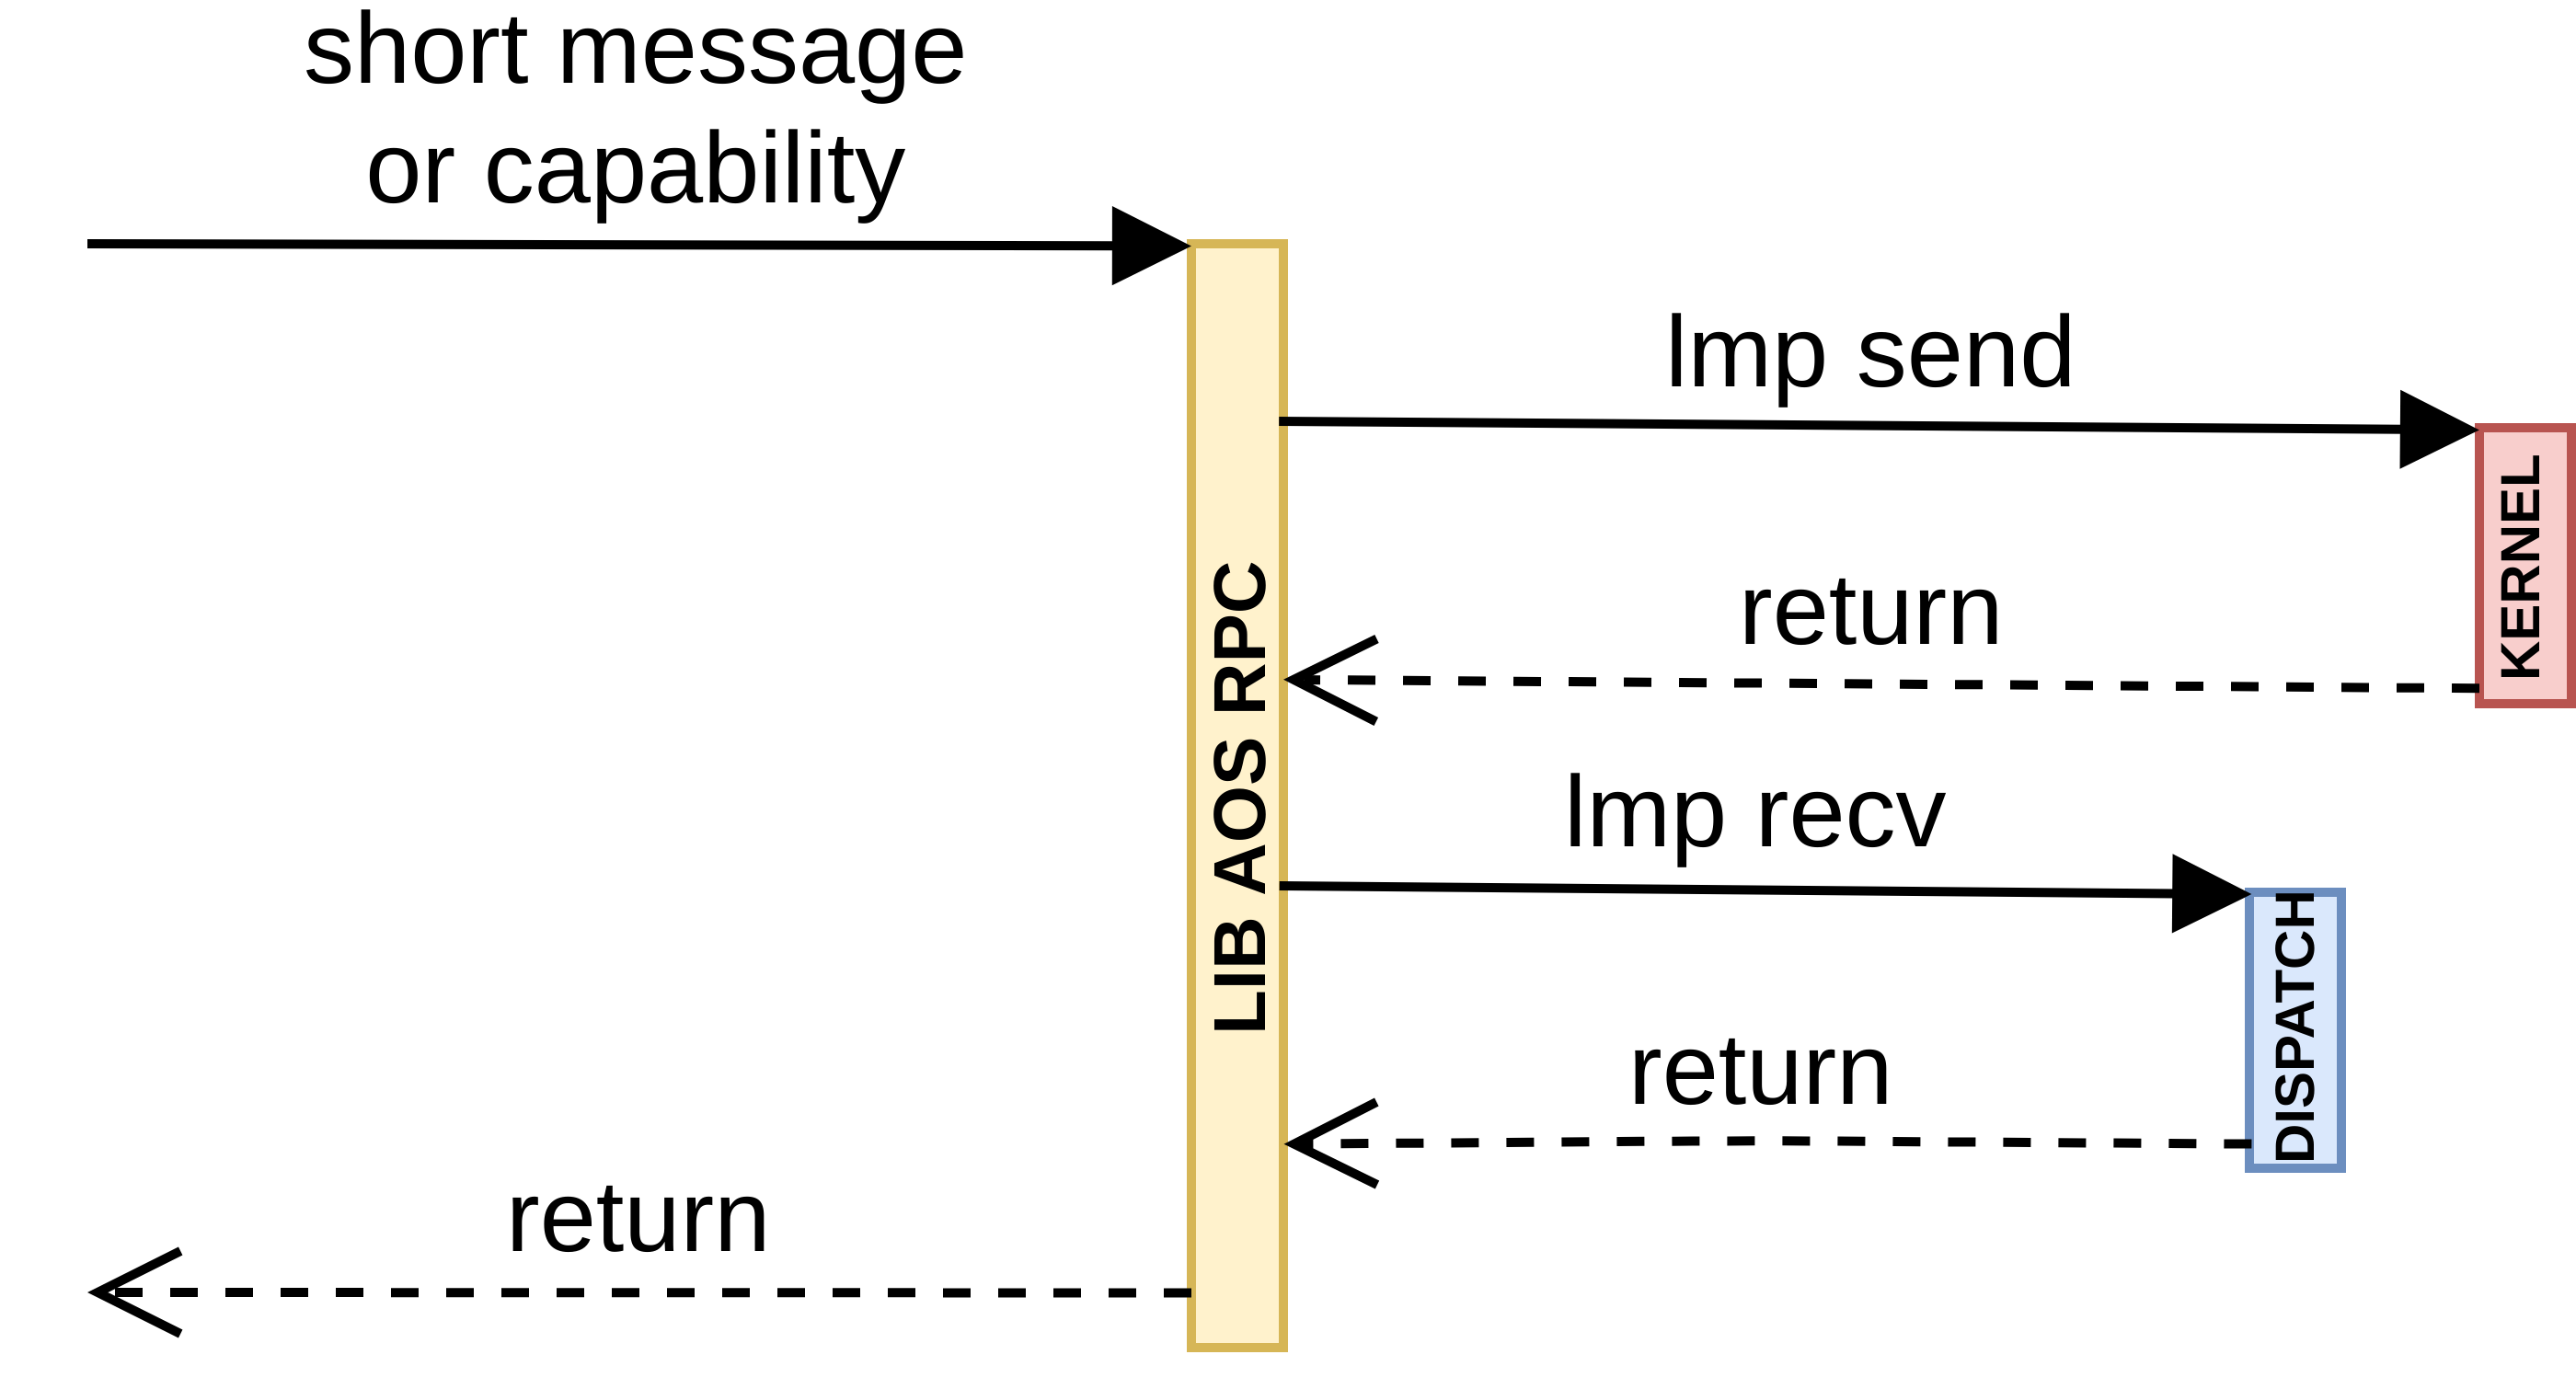
\includegraphics[width=0.7\linewidth]{assets/lmp-short}
	\caption{LMP: Short messages and/or capabilities}
	\label{fig:lmp-short}
\end{figure}

\subsection{Long Messages}
For the long messages, we basically ask init for a frame large enough to write our message into.
We then map the frame into our memory, write the message into it, and send its capability over
LMP to the destination process.
The receiving process, as soon as it receives the long messages, maps the frame into its virtual space
and is then able to read the contents of the message freely.

Long LMP messages are used for printing or reading large messages from the serial.

\begin{figure} [H]
	\centering
	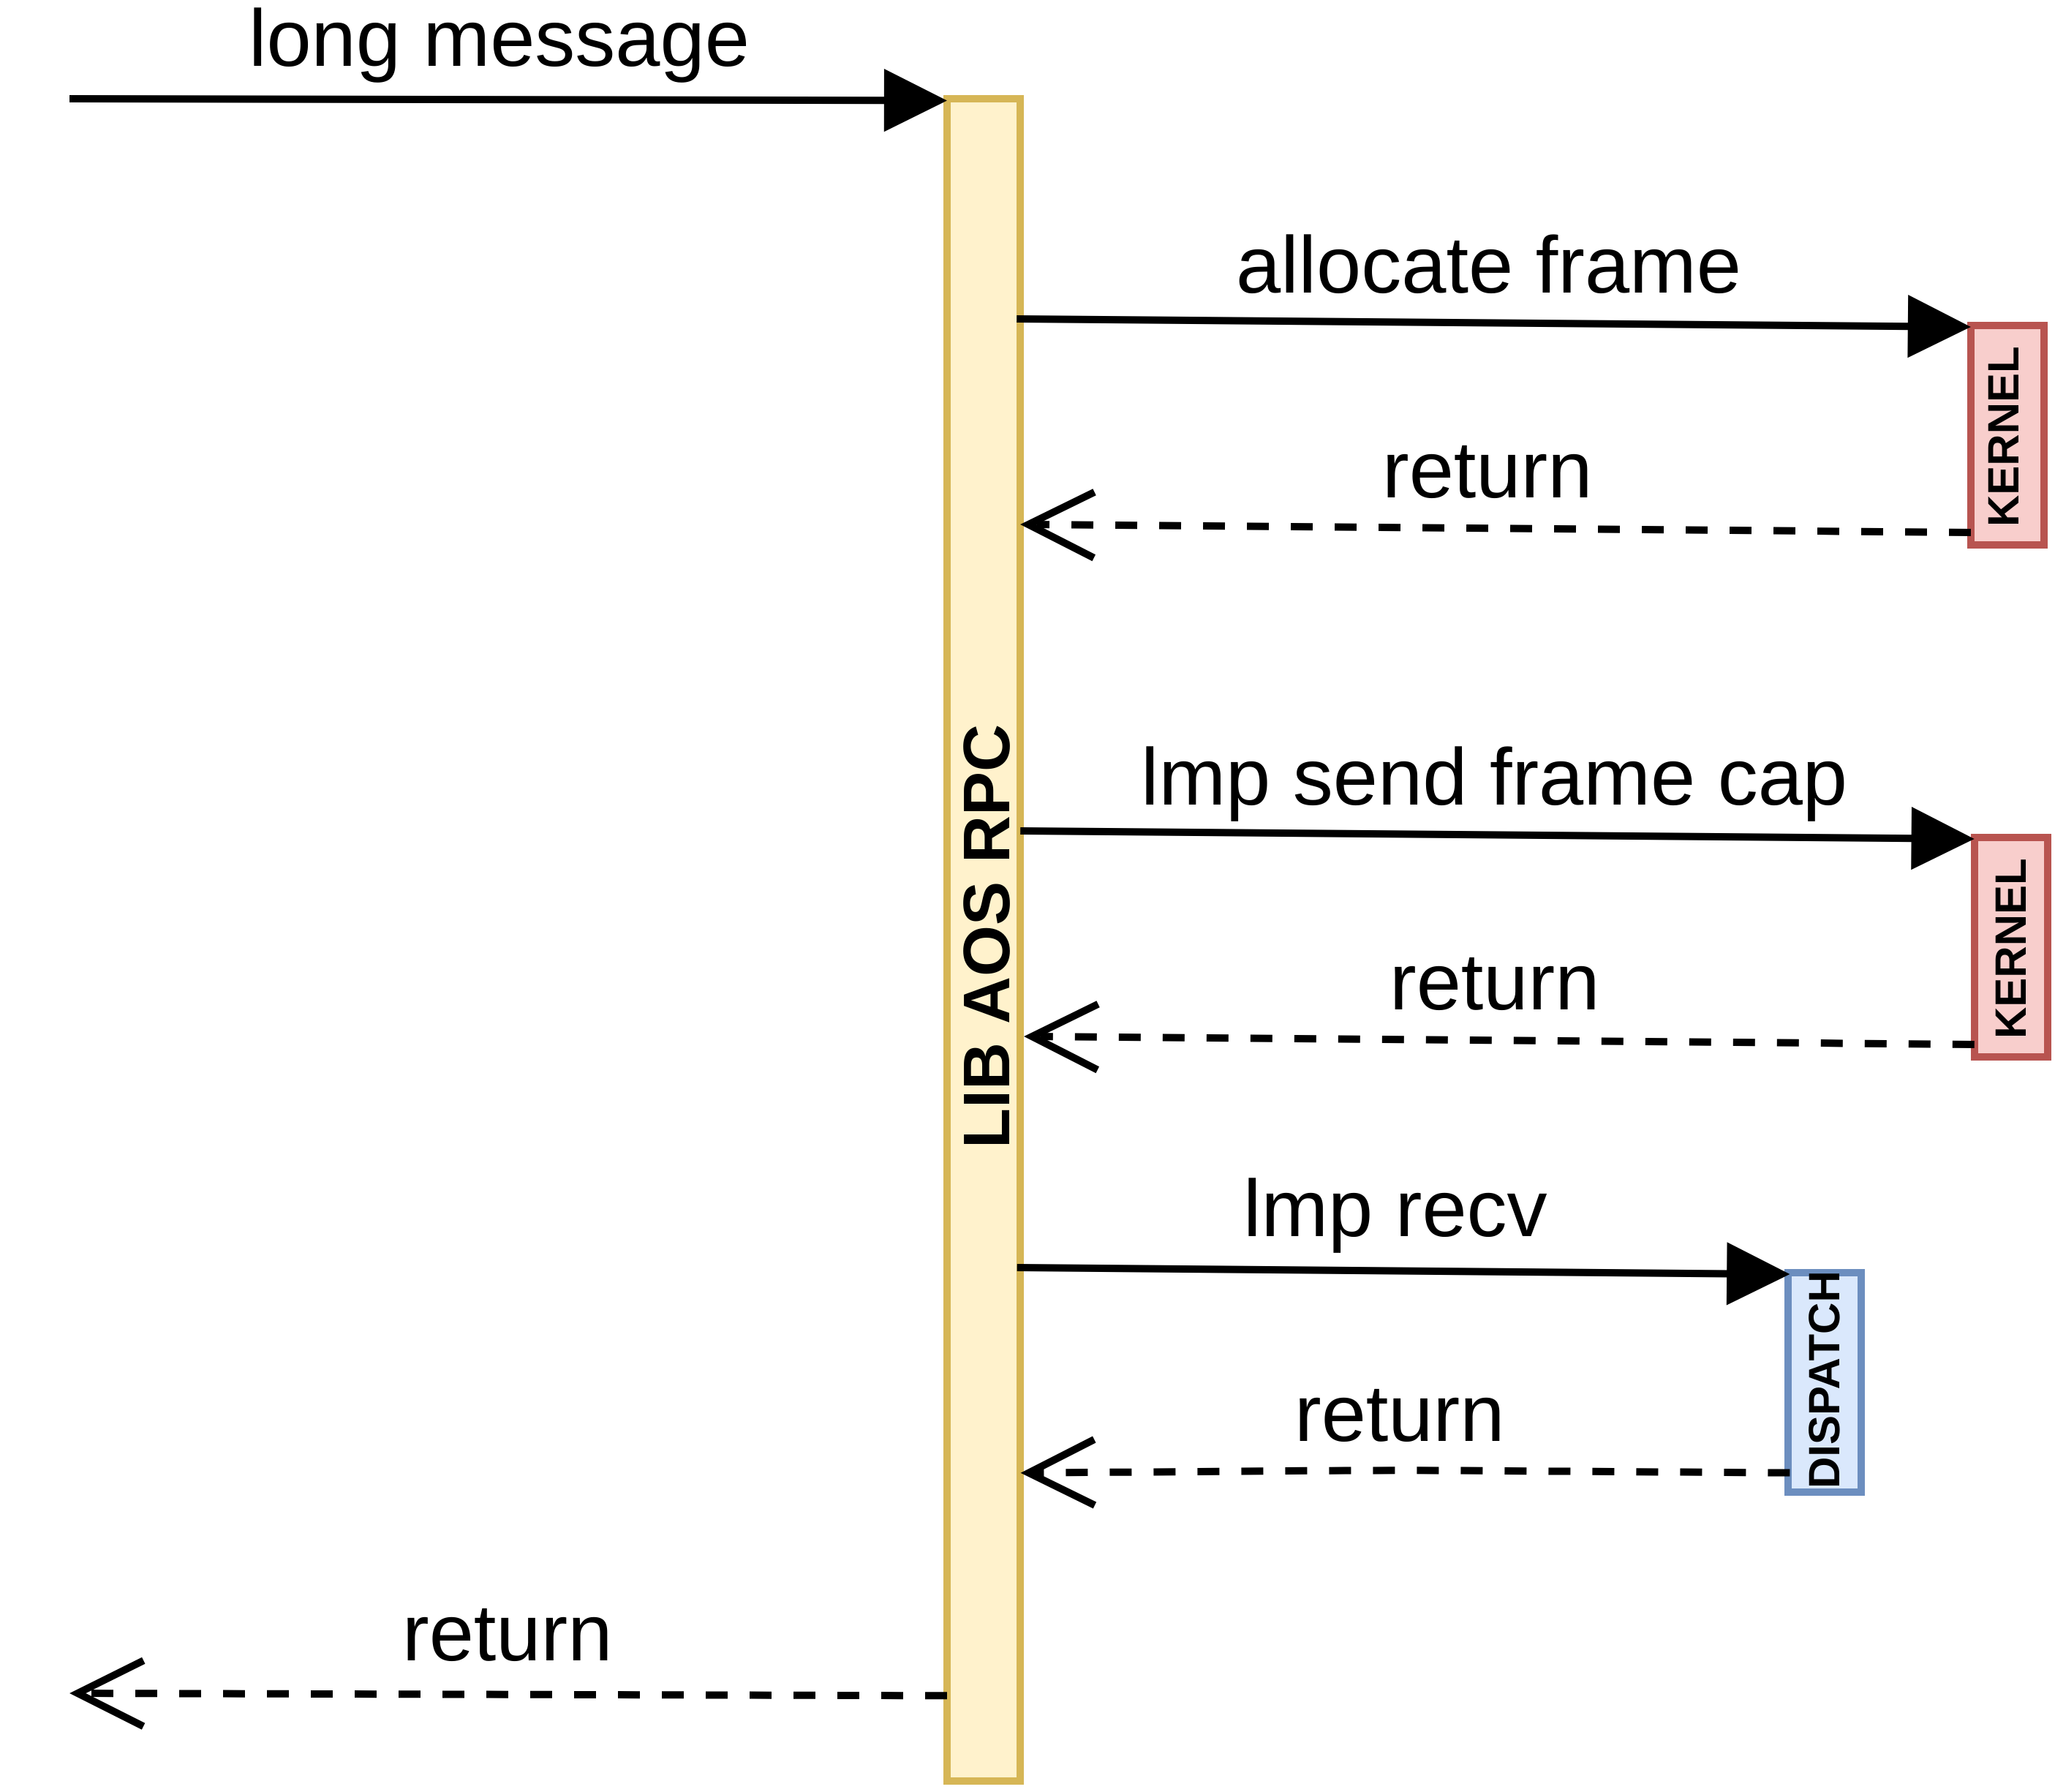
\includegraphics[width=0.7\linewidth]{assets/lmp-long}
	\caption{LMP: Messages longer than 36 bytes.}
	\label{fig:lmp-long}
\end{figure}

\newpage
\section{User-level Message Passing}
Working on multicore systems introduces new challenges for the message passing primitives. A monolithic kernel abstracts away cache coherence, maintaining (together with the hardware) the illusion of shared memory on different cores. Here we need to deal with cache coherence ourselves: 

\subsection{URPC}
URPC (User-level RPC) exploits the idea that using shared memory between two processes instead of kernel-facilitated RPC primitives can lead to better latency and throughput.

While we understand that Barrelfish's UMP and URPC are slightly different primitives, we will refer in the code to ``UMP'' as ``URPC'' - this is due to an initial misunderstanding we never managed to refactor out.

\subsection{Cache-safe Producer/Consumer Ring Buffer}
As a data structure for the UMP frame, we designed a slight variation of the one suggested in the AOS book. 

\begin{figure}[ht]
	\centering
	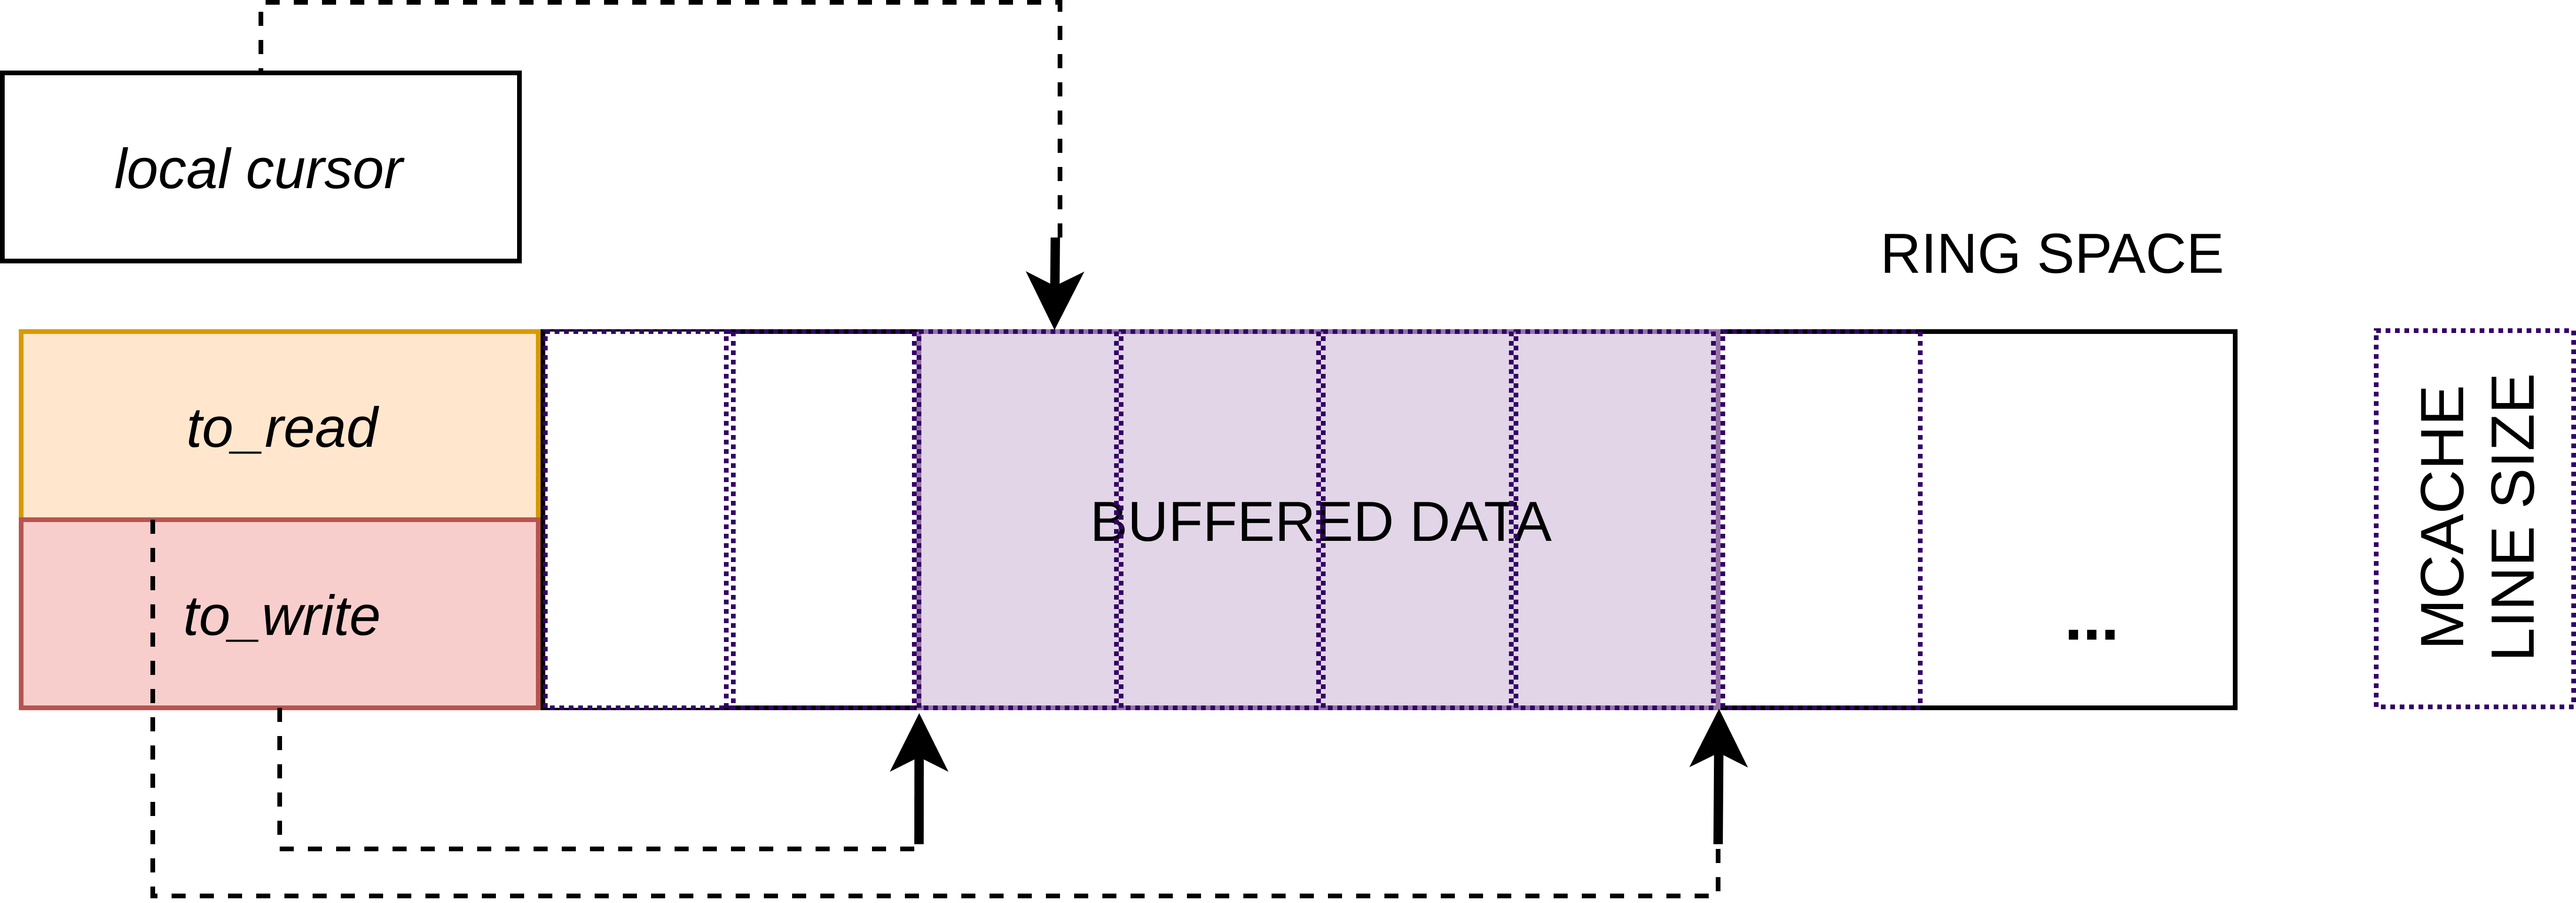
\includegraphics[width=0.9\linewidth]{assets/urpcframe}
	\caption{The shared ring buffer ("UMP Frame")}
	\label{fig:urpcframe}
\end{figure}

One of the strong point of our structure is that it makes message reassembly easier - but the performance implication were also interesting to analyze.

The buffer is split in fixed-length slots, but instead of maintaining some state word in each slot, we use two integers at the start of the shared buffer. 
The consumer will only increment the \texttt{to\_write} shared cursor (which indicates how much space is available for the writer), and keep his own local, non shared cursor to keep track of the data that has been read.
The producer will only increment the \texttt{to\_read} shared cursor (which indicates how much data needs to be read), and keep his own local, non shared cursor.

During a read, the consumer will compare its local cursor with the \texttt{to\_read} shared cursor: until they are equal, it will read the next slot, increase the local cursor and increase \texttt{to\_write} to free the slot.

Similarly the producer will compare its local cursor with the \texttt{to\_write} shared cursor: until they are equal, it will write in the next slot, increase the local cursor and increase \texttt{to\_read} to indicate new data is available.

Producer and consumer will block if they cannot advance their buffers, but they will never deadlock.

To maintain the memory consistence, data memory barriers (\textbf{dmb}) have been inserted between the reading of the shared cursors and the read/write operations on the ring space, and between those operation and the writing of the shared cursors.


\begin{pandacode}
urpc_read(): ...
while (read < n && *cursor != r_buf->s.to_read)
	// Memory barrier for reading cursor to_read
	dmb();	
	size_t min_read = MCACHE_LINE_SIZE;
	size_t pad = 0;
	if (n - read < MCACHE_LINE_SIZE)
		min_read = n - read;
		pad = MCACHE_LINE_SIZE - min_read;
	// Read data bytes
	for (int i = 0; i < min_read; i++)
		dest[read++] = r_buf->s.buf[(*cursor)++];
	for (int i = 0; i < pad; i++) 
		(*cursor)++;
		read++;
	// Memory barrier for setting cursor to_write
	dmb();	
	// Advance shared cursor
	size_t tmp = (r_buf->s.to_write + MCACHE_LINE_SIZE) % URPC_BUF_SIZE;
	r_buf->s.to_write  = tmp; // Atomic if 32bit in armv7	
	// Advance own cursor
	*cursor %= URPC_BUF_SIZE;
\end{pandacode}


\subsubsection{Performance considerations}
Each slot is sized appropriately to be contained in a cache line, and the two shared cursor - 32 bytes each - will also fit inside two cache lines.

Pooling on the cursors will therefore be cheap: the cache line containing them will be in Shared state for one side, and in Owner state for the other.

The data slot cache line will be go into \textbf{Exclusive} state in the Producer's cache as soon as it start writing - the same will happen for the shared cursor cache line when the cursor is update. Both will then transition to the \textbf{Owner} state, as the Sender pools on those lines, and a probe message over the cache inter-connect will be produced.

We therefore estimate that, for a \emph{single cache-line sized write}, four round-trip on the interconnect are needed (invalidate and probe, for both the cursors cache lines).
For \emph{bigger writes}, on the other hand, this data structure stars to be more efficient: particularly if the one of the producer and the consumer speed is asymmetric, the number of round-trips on the interconnect for the cursors will grow less then linearly - in some cases the producer will update the shared cursor multiple times, while it is in a cache line in the Exclusive state, before actually transitioning to Owner.

Due to our time constraints we were not able to perform comparative benchmarks - we currently have no data supporting our performance estimation.


\subsection{Binding}
Now that we have UMP primitives available, we can build a system to make it easy for dispatcher to set up an UMP channel between them.

The book suggested a client-server architecture - we decided to go for a simpler publisher-subscriber model.

The server announces ... and the client registers
diagram

This architecture was easier to code, required a simpler channel setup and fitted our use case - where a few dispatchers carrying out system functionalities, like the file system and the network stack, publish services for the rest of the system to use. A complete (and more flexible) client-server architecture would have been a good choice if we had a working nameserver.

\newpage
\subsection{LMP Long messages}
Many parts of the systems can benefit of the speed of passing data on a UMP frame - one of those is the LMP Long messages handling.

\begin{figure}[ht]
	\centering
	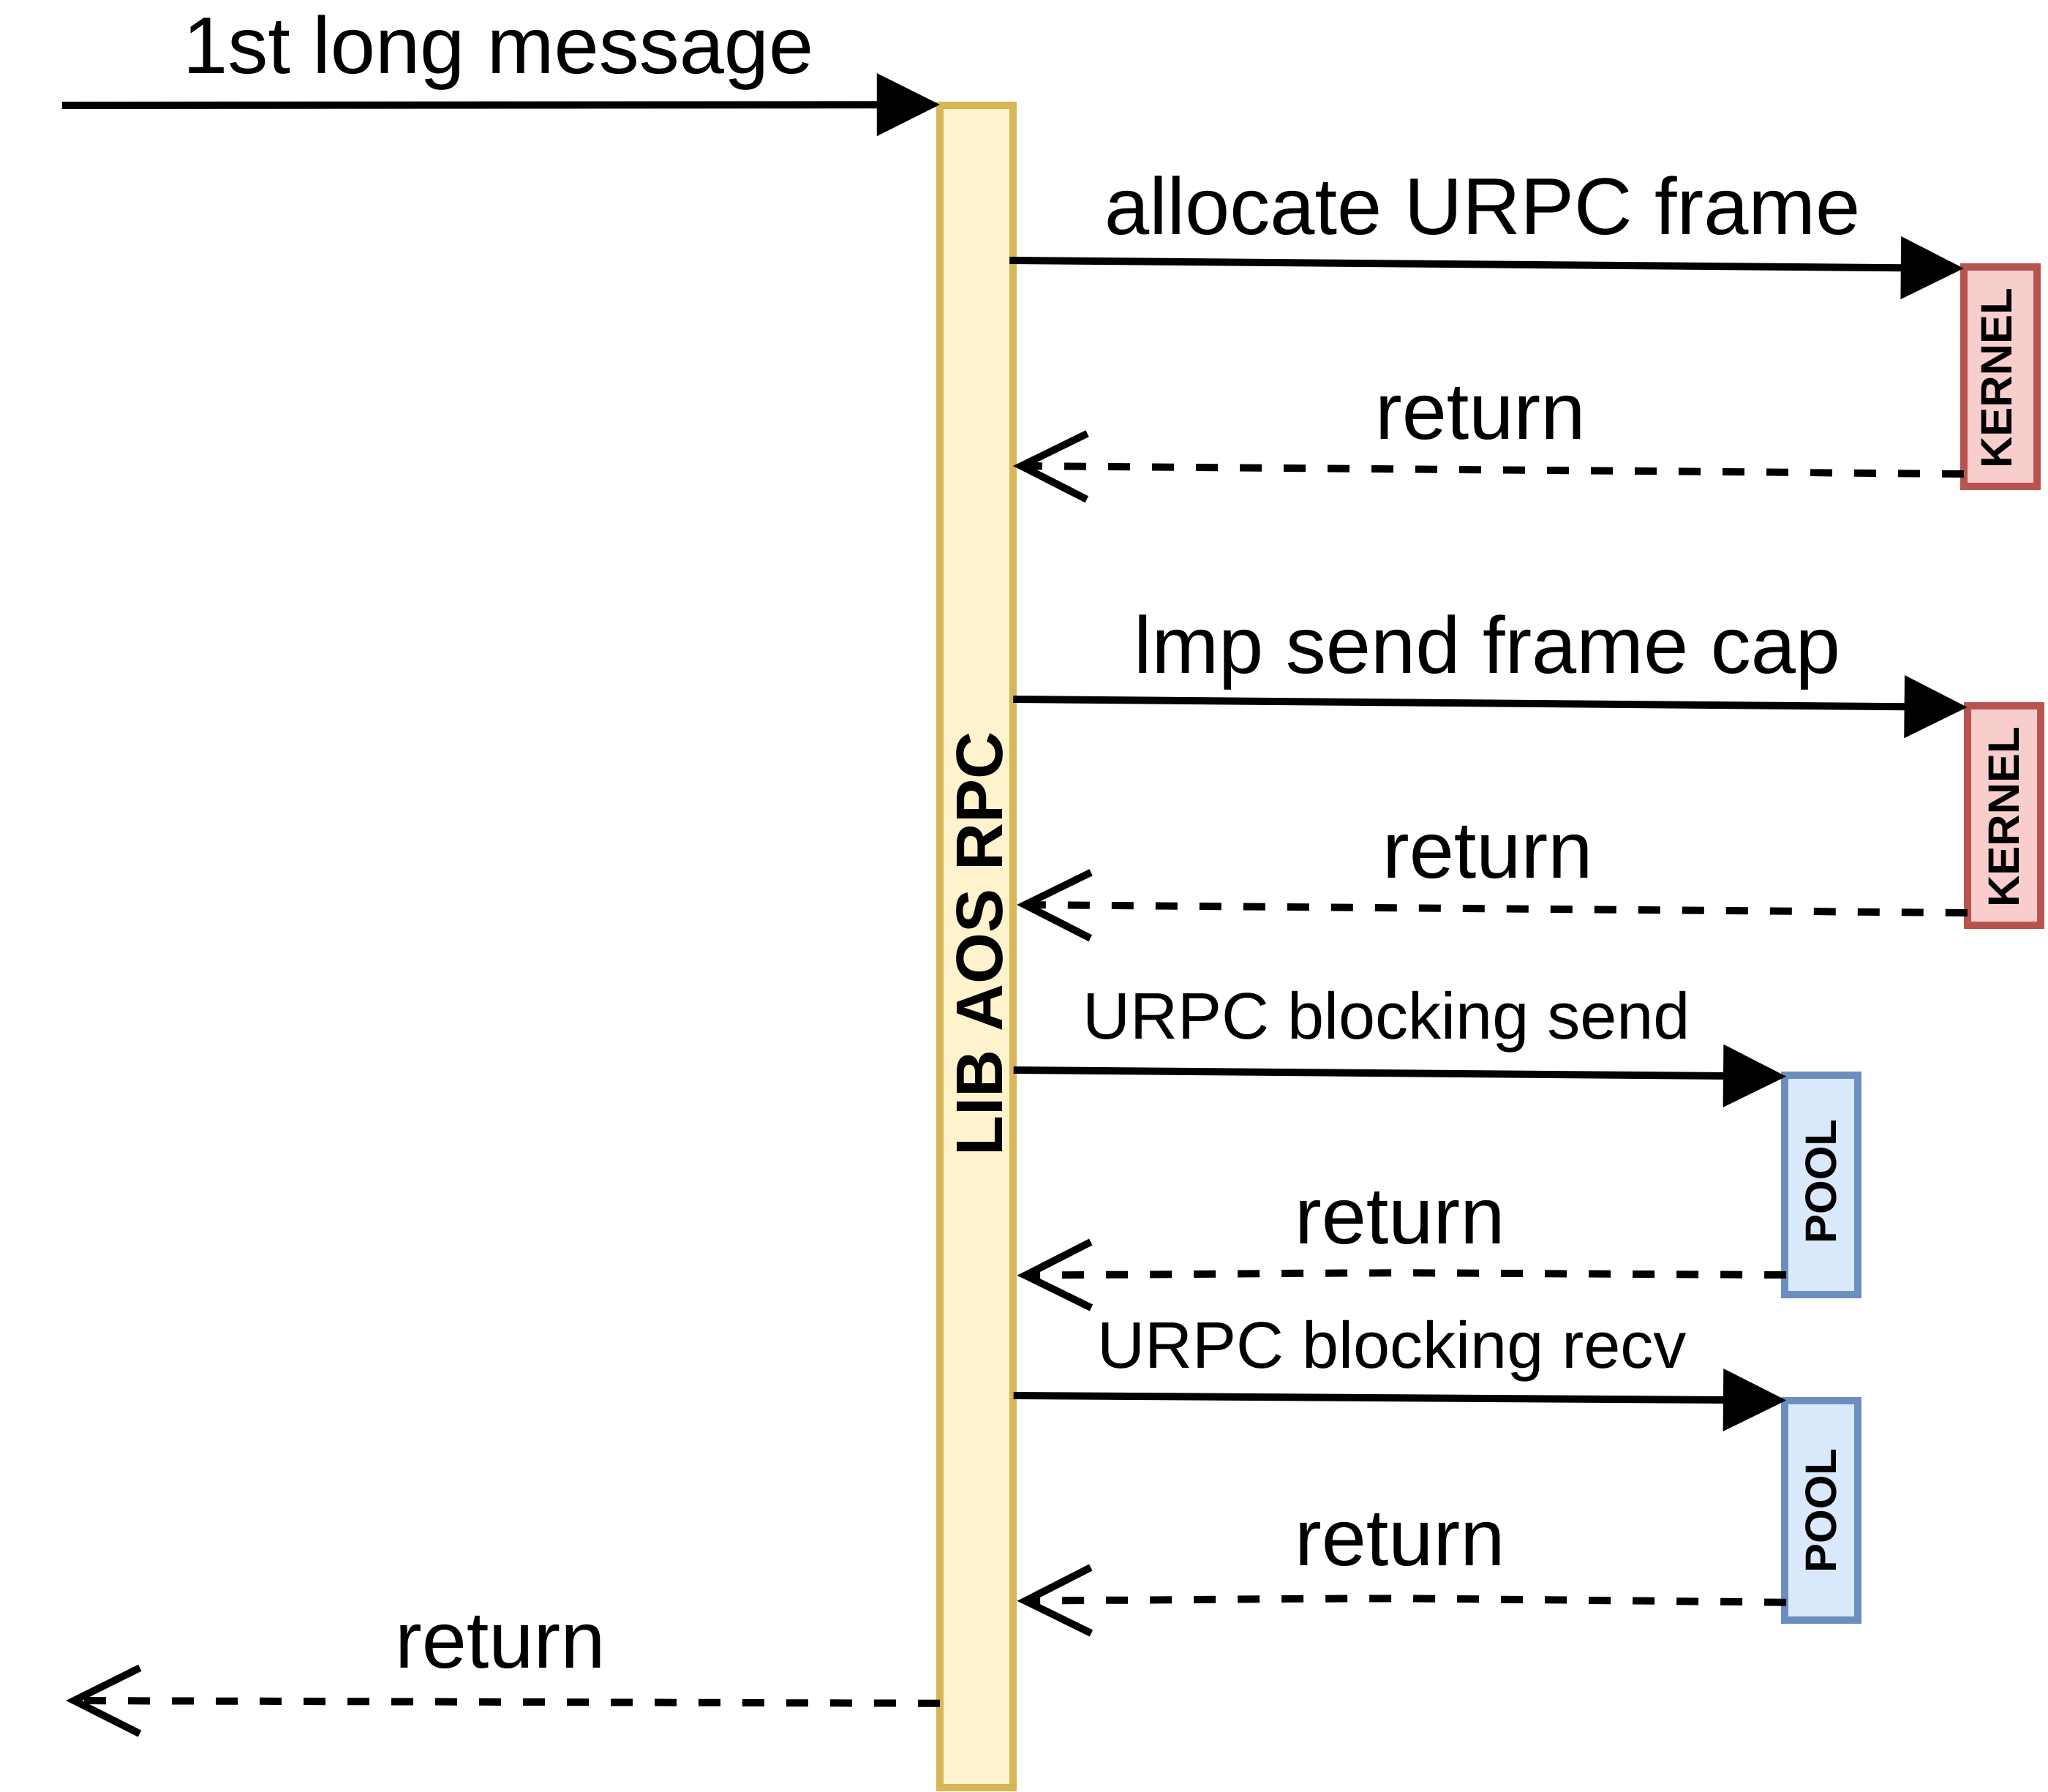
\includegraphics[width=0.7\linewidth]{assets/lmp-long-urpc-first}
	\caption{The first long message on a certain channel is sent - the frame is created on-demand.}
	\label{fig:lmp-long-urpc-first}
\end{figure}

Many parts of the systems can benefit of the speed of passing data on a UMP frame - one of those is the LMP Long messages handling.
Instead of creating an had-oc frame for each long message, we only create one frame per channel. The frame is created on-demand on the first long message, and exchanged using the usual \texttt{aos\_rpc\_send\_capbuf} (figure \ref{fig:lmp-long-urpc-first})- but after this first exchange, we use a blocking write on the UMP frame to send messages, and a blocking read to receive (figure \ref{fig:lmp-long-urpc}).

\begin{figure}[ht]
	\centering
	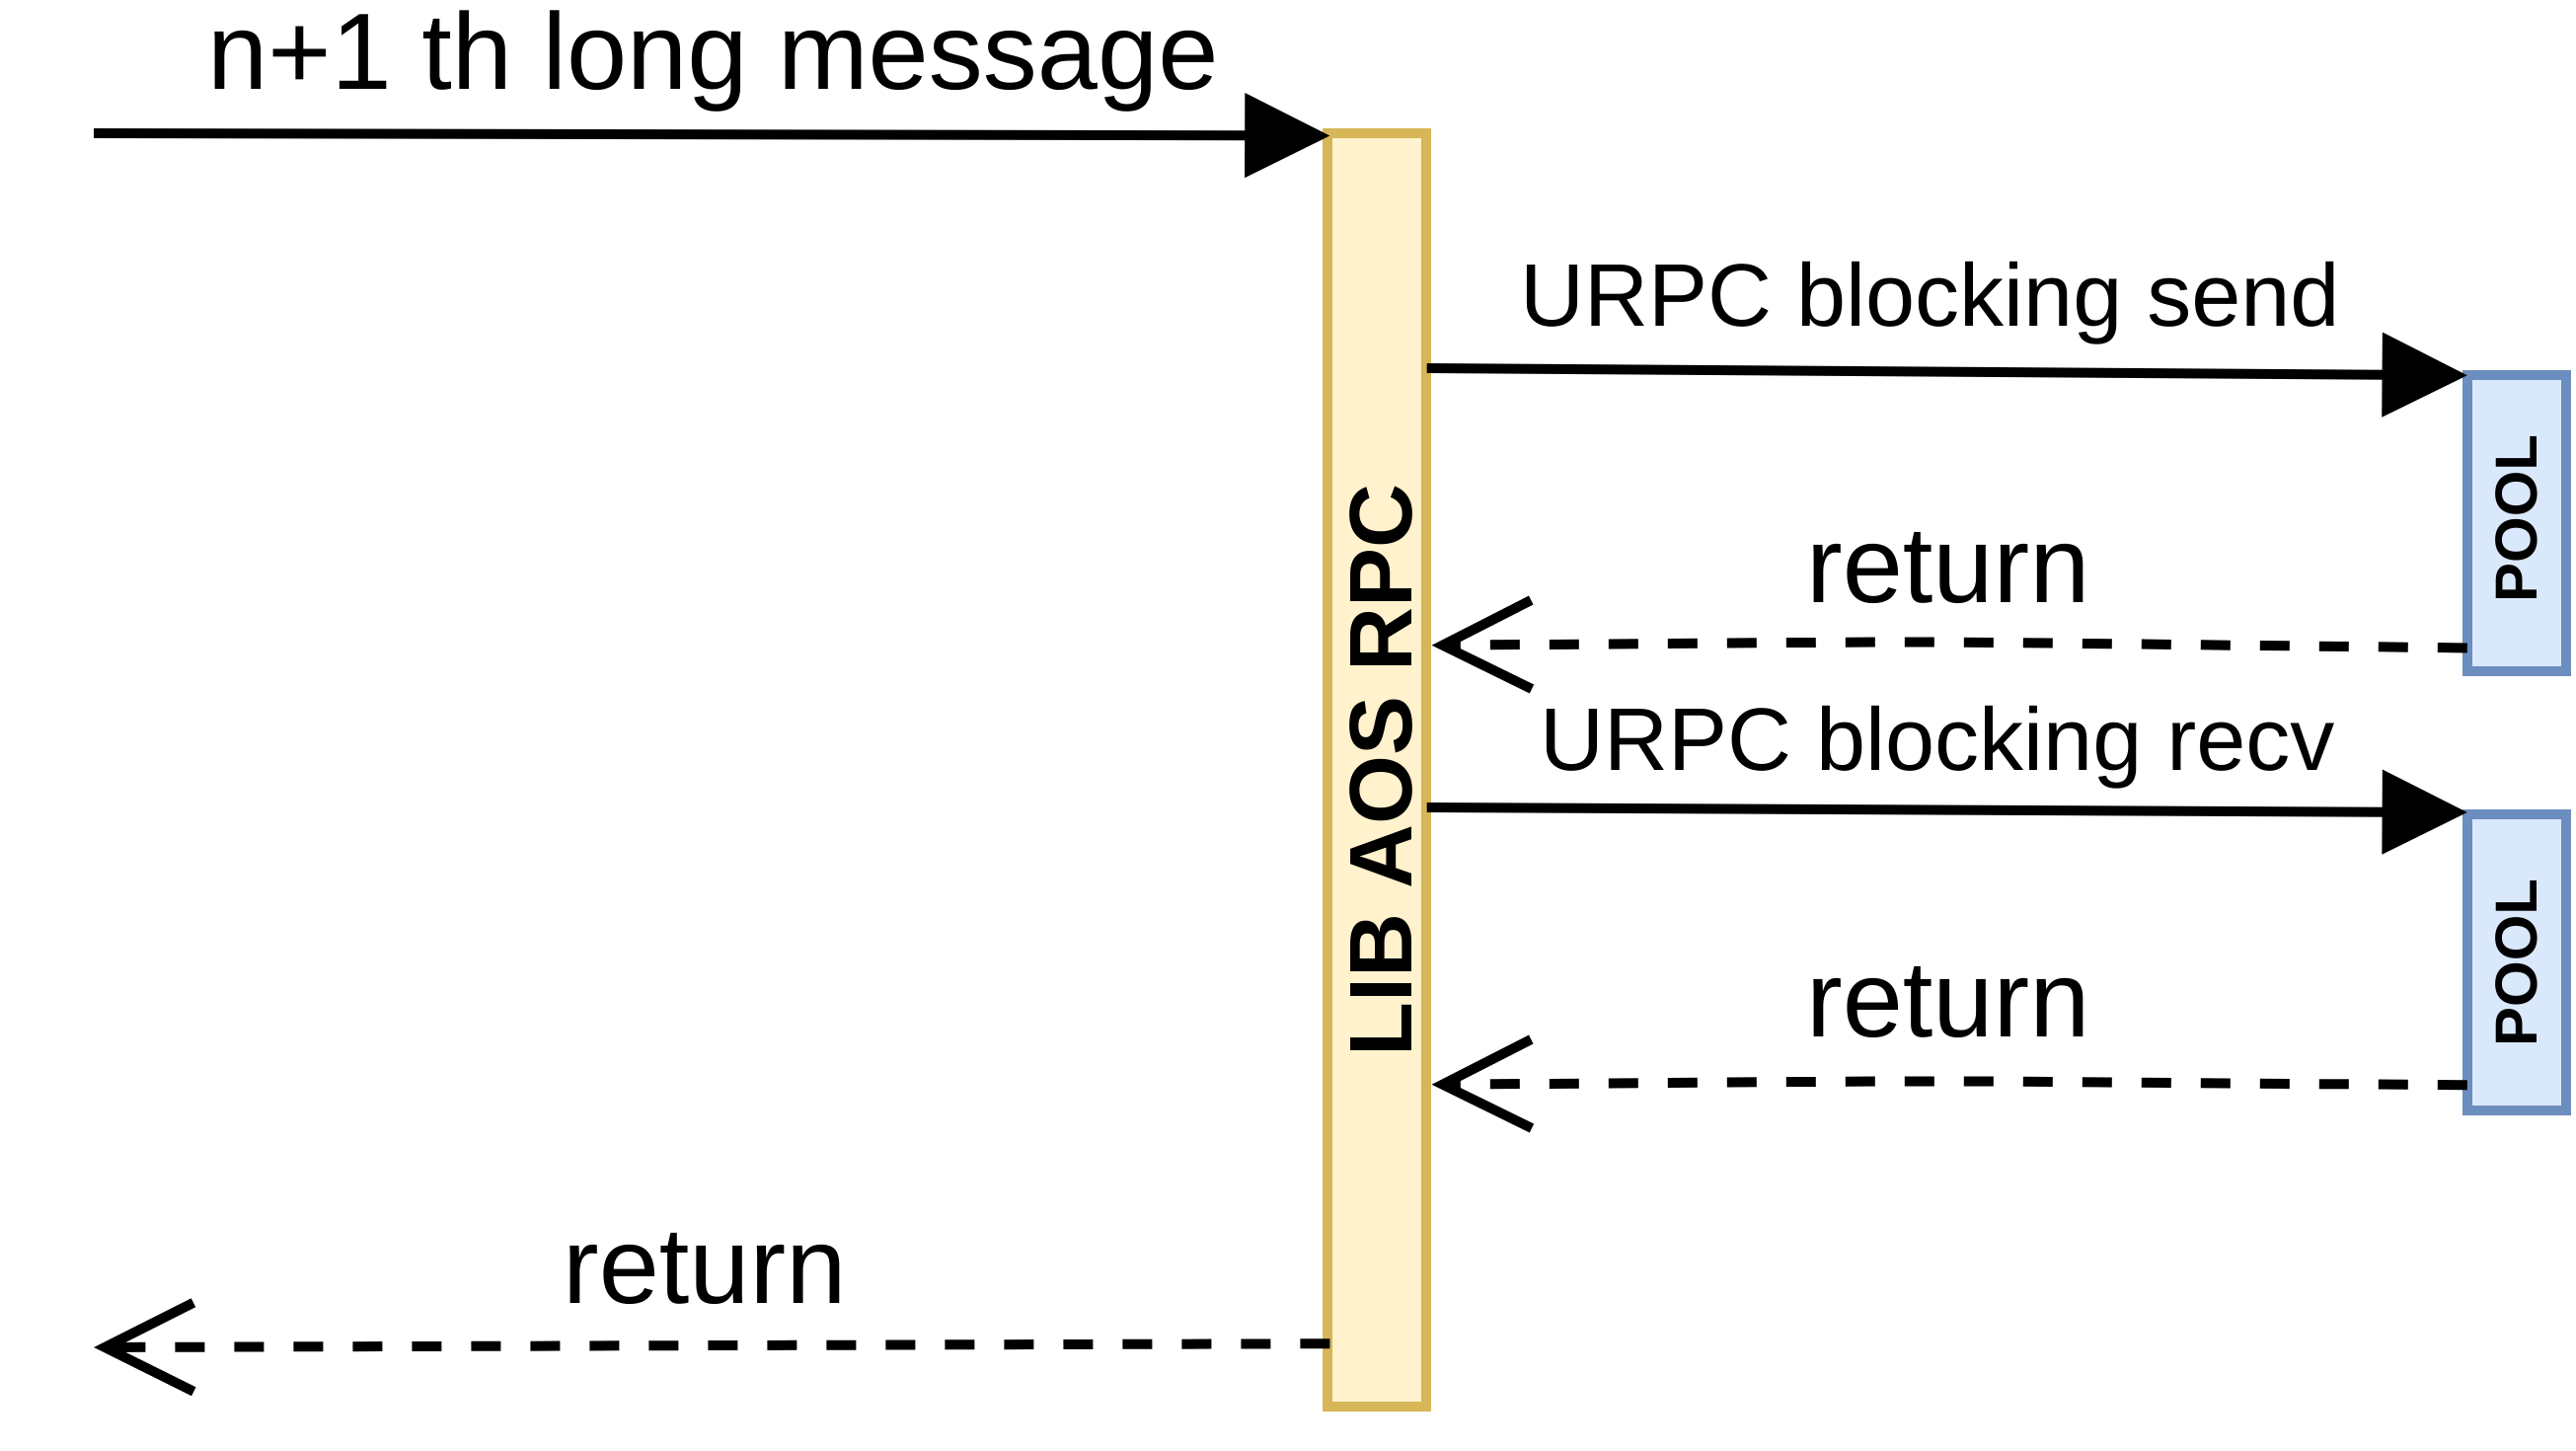
\includegraphics[width=0.7\linewidth]{assets/lmp-long-urpc}
	\caption{Any subsequent long message on the same lmp channel uses the available UMP frame - never entering the kernel.}
	\label{fig:lmp-long-urpc}
\end{figure}

\begin{pandacode}
aos_rpc_send_req(): ..
req.longreq = true; req.len = len;
if (!chan->longreq_urpc_init) 
	struct capref frame;
	err = frame_alloc(&frame, BASE_PAGE_SIZE, NULL);
	chan->longreq_frame = frame;	
	err = urpc_map(frame, &chan->longreq_urpc);
	err = aos_rpc_send_capbuf(chan, req.bytes, RPC_MAX_LEN, frame);
	chan->longreq_urpc_init = true;
else
	err = aos_rpc_send_capbuf(chan, req.bytes, RPC_MAX_LEN, NULL_CAP);
urpc_write_msg(&chan->longreq_urpc, (char *) buf, len);
\end{pandacode}

The performance improvement was sensible. The trade-off of the current implementation is that pooling on many UMP frames can become expensive - in a future development iteration, we reserve to measure the performance impact of using LMP for signaling when a message is available instead of pooling on the UMP frame directly.

In the current use cases, there are very few channels being used, and most of the time an UMP call expects and immediate response (or no response at all) - in which case we believe the additional latency of LMP would outweigh the impact of pooling on the CPU.



\section{LMP over UMP}
For achieving complete Remote Procedure Call functionalities, we decided to offer a way for dispatchers to have their LMP requests transparently transferred and routed to the other core. This is implemented by having the monitor share an UMP frame with the init dispatcher running on the second core's CPU driver (the \emph{remote monitor}).

When an RPC request is received, each monitor checks whether it should be routed to the other core - in which case it sends it, marshalled in the very same data structure as LMP, over the UMP frame. On the other side the monitor waits for messages on the UMP channel, and runs the same request handler used by the LMP.

Our LMP was generic enough to serve both ends, and we introduced a level of indirection on the \texttt{aos\_rpc\_channel} structures, allowing them to support both LMP and UMP functionality.


\begin{figure} [ht]
	\begin{pandacode}
struct aos_rpc 
	struct lmp_chan lc;
	struct waitset* ws;
	struct thread_mutex mutex;
	
	errval_t (*send_raw_f)(struct aos_rpc*, const char *,
				size_t, struct capref);
	errval_t (*send_req_f)(uint8_t type, struct aos_rpc*, const char *,
				size_t, struct capref);
	errval_t (*rec_raw_f)(struct aos_rpc*, char *,
				size_t*, struct capref*);
	errval_t (*rec_req_f)(uint8_t *, struct aos_rpc*, char **,
				size_t*, struct capref*);
				
	void * ancillary;
	
	bool longreq_urpc_init;
	urpc_s longreq_urpc;
	struct capref longreq_frame;
\end{pandacode}
	\caption{This extract of code shows the generic \texttt{aos\_rpc} data structure, with a vtable-like section and a generic \textit{ancillary data} pointer implementing some very basic polymorphism.}
\end{figure}

While convenient, this approach introduced several problems: 
\begin{itemize}
	\item LMP sending is asynchronous, while all the operations on the UMP channel are synchronous and blocking;
	\item handling requests over the UMP channel introduces concurrency;
	\item messages from different LMP channels are flattened in a single UMP channel.
\end{itemize}

In the next sections, we will describe how we tackled those issues.

\subsection{LMP locking}
For handling bot the LMP and the UMP channels at the same time, the monitor spawns a second thread that pools on the UMP frame. This introduces concurrency in some parts of the code that were not designed to be thread safe.

We introduced granular locks and made most of the code thread safe.
Yet, some more subtle and hard to debug errors seem to have persisted - once in 10 or more boots, the kernel hangs inexplicably.

\subsection{Asyncronous responses}

Most of our RPC requests sent a request over the LMP channel, and then set up a listener that would have upcalled the process when a response was ready. This is no longer possible on the UMP channel. Moreover, the fact that sever channels are multiplexed into one means that the monitor cannot simply lock the UMP channel when waiting for a response - it would risk a deadlock if some other request needs to use the UMP to be handled.
 
Using proper sessions for channel multiplexing/demultiplexing would probably had been a good choice, but we decided to implement a more basic and simple callback mechanism.
\begin{figure} [H]
	\begin{pandacode}
case RPC_REMOTE_RES:
	rpc_res *res = (rpc_res*) buf;
	size_t res_type = res->args.res_type;
	struct urpc_cb_s *cb = dlist_head(&urpc_cb_queues[res_type]);
	if (cb == NULL) 
	debug_printf("\x1b[1mNo callback was set "
	"for this response!\x1b[0m - %d\n",
	es->args.res_type);
	break;
	cb->f(cb->args, cb->chan, (rpc_res*) buf);
	dlist_remove(&urpc_cb_queues[res_type], cb);
	free(cb);
	\end{pandacode}
	\caption{A code extract from the callback implementation: this is a case of the switch handling the different types of RPC request. If the type matches the special type \texttt{RPC\_REMOTE\_RES}, a callback is selected according to the type of the response.}
\end{figure}
When the monitor detects a request that needs to be routed to the \emph{remote monitor}, it first sets up a callback for a \emph{remote response} and then sends the request on the UMP channel. On the other side, the remote monitor will receive and handle the request like a local LMP RPC, but thanks to the polymorphic \texttt{aos\_channel} the reply will be sent over UMP. Back on the first monitor, the remote response will trigger the callback.



\chapter{Multicore}
\section{Booting the second core}

The code relative to boot the second core can be found in file \t{lib/spawncore/spawncore.c}, 
in function \t{spawn\_core()}.

This is done in the following steps:

\subsection{Function \t{setup\_core\_data()}}
Here we prepare the necessary memory and capabilities required to call
\t{invoke\_kcb\_clone()}. This clones the current \emph{kernel control block},
and partially fills up the \t{core\_data} struct.

We need a frame big enough to store the cloned \emph{kcb}. The precise
size can be obtained with \t{sizeof (struct arm\_core\_data)}. Also,
we need a capability for the cloned \emph{kcb}; this can be a capability
retyped from a \t{RAM\_CAP} with type \t{ObjType\_KernelControlBlock} 
of size \t{OBJSIZE\_KCB}. We can then pass the capability and the frame
to the \t{invoke\_kcb\_clone()} function. Lastly, we set the 
\t{core\_data->kcb} pointer to the physical address of the \emph{kcb} capability.

\begin{pandacode}
	size_t core_data_size;
	struct capref core_data_frame; 
	err = frame_alloc(&core_data_frame, sizeof(struct arm_core_data), &core_data_size);
	DBGERR(err, "Error allocating frame for core data on core boot\n");
	...
	err = paging_map_frame_attr(get_current_paging_state(), 
	core_data_buf, core_data_size, core_data_frame, 
	VREGION_FLAGS_READ_WRITE, NULL, NULL);
	DBGERR(err, "Error mapping core data struct frame\n");
	...
	// Getting a KCB
	struct capref ram_cap; 
	err = ram_alloc(&ram_cap, OBJSIZE_KCB);
	...
	err = slot_alloc(kcb);
	err = cap_retype(*kcb, ram_cap, 0, ObjType_KernelControlBlock, OBJSIZE_KCB, 1);
	DBGERR(err, "Error retyping ram cap to KCB\n");
	invoke_kcb_clone(*kcb, core_data_frame);
	...
	struct frame_identity fi;
	err = frame_identify(*kcb, &fi);
	DBGERR(err, "Error identifying kcb\n");
	(*core_data_s)->kcb = fi.base;
\end{pandacode}


\subsection{Function \t{setup\_core\_monitor()}}
Now we must load the ELF file for init. This function searches the multiboot
image for a module called \t{"armv7/sbin/init"}, allocates the required memory
(\t{ARM\_CORE\_DATA\_PAGES * BASE\_PAGE\_SIZE * 2}) and inside the struct
\t{core\_data} sets the pointers to the location of init's ELF and the location
of the newly allocated memory. It also sets the \t{core\_data->cmdline} pointer
to its correct value to ensure that the newly spawned init will have its
command line arguments.

\begin{pandacode}
	// Setting up core data monitor fields
	size_t retbytes;
	struct mem_region* init_mm_reg = multiboot_find_module(bi, "armv7/sbin/init");
	struct multiboot_modinfo init_mod = {
		.reserved   = 0,
		.mod_start  = init_mm_reg->mr_base, 
		.mod_end    = init_mm_reg->mr_base + init_mm_reg->mrmod_size,
		.string     = init_mm_reg->mrmod_data,
	};
	core_data_s->monitor_module     = init_mod;
	
	// Allocating frame for init on other core
	struct capref init_frame; 
	err = frame_alloc(&init_frame, 2*ARM_CORE_DATA_PAGES*BASE_PAGE_SIZE, &retbytes);
	DBGERR(err, "Error allocating frame for init on core boot\n");
	
	//Setup core data init fields
	struct frame_identity init_fi;
	err = frame_identify(init_frame, &init_fi);
	DBGERR(err, "Error identifying init frame\n");
	strncpy(core_data_s->init_name, monitor_name, DISP_NAME_LEN + 1);
	core_data_s->memory_base_start = init_fi.base;
	core_data_s->memory_bytes = init_fi.bytes;
	core_data_s->cmdline = core_data_fi.base + offsetof(struct arm_core_data, cmdline_buf);
\end{pandacode}

\subsection{Function \t{setup\_cpu\_driver()}}
It's time to load the cpu driver into memory. The cpu\_driver is different
depending on if we are going to run it on the panda board or virtualized
through QEMU. To support this, we first look for the \t{"cpu\_omap44x"} module
in the multiboot image. If that is not found (the function
\t{multiboot\_find\_module()} returns \t{NULL}), then we look for the
\t{"cpu\_a15ve"} module.  After that, we allocate enough space for the cpu
driver and map it in memory:
\begin{pandacode}
	errval_t err;
	struct mem_region* cpu_driver_mm_reg;
	
	if ((cpu_driver_mm_reg = multiboot_find_module(bi, "cpu_omap44xx")) != NULL) {
		HARDWARE = 1;
	} else if ((cpu_driver_mm_reg = multiboot_find_module(bi, "cpu_a15ve")) != NULL) {
		HARDWARE = 0;
	} else { USER_PANIC("Unknown hardware\n"); }
	
	struct capref cpu_driver_frame = {
		.cnode  = cnode_module,
		.slot   = cpu_driver_mm_reg->mrmod_slot,
	};
	struct frame_identity cpu_driver_fi;
	frame_identify(cpu_driver_frame, &cpu_driver_fi);
	paging_map_frame_attr(get_current_paging_state(),
	cpu_driver_addr, cpu_driver_fi.bytes, cpu_driver_frame, 
	VREGION_FLAGS_READ_WRITE, NULL, NULL);
\end{pandacode}
Before continuing, we also need to prepare the relocation segment. This is
easily done by calling the provided \t{load\_cpu\_relocatable\_segment()}, 
we just had to allocate and map the necessary memory:
\begin{pandacode}
// Allocate space for relocation of the cpu driver ELF
struct capref reloc_seg_frame;
size_t reloc_seg_size;
err = frame_alloc(&reloc_seg_frame, cpu_driver_fi.bytes, &reloc_seg_size);
DBGERR(err, "Error allocating frame for reloc segment\n");

err = paging_map_frame_attr(get_current_paging_state(),
reloc_seg_addr, reloc_seg_size, reloc_seg_frame,
VREGION_FLAGS_READ_WRITE, NULL, NULL);
DBGERR(err, "Error mapping relocation segment frame\n"); 

// Load relocatable segment of the cpu driver
struct frame_identity reloc_fi;
err = frame_identify(reloc_seg_frame, &reloc_fi);
err = load_cpu_relocatable_segment(*cpu_driver_addr, *reloc_seg_addr, reloc_fi.base,
core_data_s->kernel_load_base,
&core_data_s->got_base);
\end{pandacode}

\subsection{Function \t{setup\_core\_urpc()}}
Here we write into the global capref \t{cap\_urpc} the capability of a newly
allocated frame that will serve the purpose of being the shared frame between cores.
We then calculate the physical address and size of that frame with a call to
\t{frame\_identify()} and set the corrisponding pointers
\t{core\_data->urpc\_frame\_base} and \t{core\_data->urpc\_frame\_size}.
Finally, we map that frame into the first core's virtual memory. The resulting
virtual address will then be used by function \t{urpc\_s\_init()} as explained
in the previous chapter:
\begin{pandacode}
// Setup core data URPC fields
err = frame_alloc(&cap_urpc, BASE_PAGE_SIZE, NULL);
DBGERR(err, "Error allocating frame for cap urpc\n");
struct frame_identity urpc_fi;
err = frame_identify(cap_urpc, &urpc_fi);
DBGERR(err, "Error identifying core_data\n");
core_data_s->urpc_frame_base    = urpc_fi.base;
core_data_s->urpc_frame_size    = urpc_fi.bytes;

err = paging_map_frame_attr(get_current_paging_state(), 
	(void **) urpc_buffer, 0x1000,
cap_urpc, VREGION_FLAGS_READ_WRITE, NULL, NULL);
DBGERR(err, "Urpc frame mapping failed");
\end{pandacode}



\subsection{Spawning the core}
In the end, we can call the syscall \t{invoke\_monitor\_spawn\_core}, passing as
arguments the ID of the core we want to spawn, the cpu type (for now hardcoded to
\t{CPU\_ARMV7}, and the base address of the just completed \t{core\_data} struct.

But, before that, we need to address an important point: the second core won't have the
MMU available. This means that any writes we made to the cache which weren't propagated
to the main memory will not be visible to the second core during boot. 
To ensure all writes are propagated, we clean off the cache using the 
syscall \t{sys\_armv7\_cache\_clean\_poc()}, which takes as argument an interval of 
physical addresses. The syscall ensures that the writes relative to those addresses will
be propagated. We provide the location of the newly created kernel control block:
\begin{pandacode}
struct frame_identity core_data_fi;
struct capref core_data_frame; 
err = frame_alloc(&core_data_frame, sizeof(struct arm_core_data), &core_data_size);
DBGERR(err, "Error allocating frame for core data on core boot\n");
...
err = frame_identify(core_data_frame, core_data_fi);
DBGERR(err, "Error identifying core_data\n");
...
(void*)(uint32_t) (core_data_fi.base + core_data_fi.bytes - 1));
sys_armv7_cache_clean_poc((void*)(uint32_t) core_data_fi.base, 

err = invoke_monitor_spawn_core(core_id, CPU_ARM7, core_data_fi.base);
DBGERR(err, "Error invoking monitor_spawn_core\n");
\end{pandacode}

\section{Memory management between cores}

We had to decide how to manage the split of the memory between the cores. We had two options available:
\begin{itemize}
	\item Use a predefined split of the memory equally between the cores, giving each 512 MB of RAM.
	\item Run a separate process on core 0 that gives memory on-demand to process on both
	cores.
\end{itemize}
It was obvious that the second choice would have been more elegant and extensible; however, we had to go with the first one. 
The reasons behind this decision were not based only on the lower complexity of the predefined
split and thus of the small amount of time needed to implement it, but also on the fact that 
having to \t{frame\_forge} on-demand would be much more error-prone - and bugs caused by a 
wrong usage of \t{frame\_forge} would have been very hard to catch. Also, we were worried about
performance: in case we went with the standalone memory manager option, every process on the
second core had to perform a URPC request to get its allocation requests, and would have been
much slower than having some RAM ready on its core.

\subsection{Passing the bootinfo structure}

A somewhat tricky challenge to get right was making sure that the monitor of the second core
received and used correctly the \t{bootinfo} struct. 

The \t{bootinfo} struct get written into the URPC frame by the first core just before calling \t{invoke\_monitor\_spawn\_core()}; the monitor (\t{init}) on the second core will receive 
it through a call to \t{urpc\_read\_msg()} as the first thing in its \t{main()} function.

After that, the monitor will go through the regions of the second core, forging the ram
capabilities corresponding to the regions indicated in the bootinfo which were not consumed
already by the first core, storing those capabilities inside the \t{cnode\_super} cnode.

We're still not done: the second core must know the name of the modules inside the
multiboot image, contained inside the \t{modstrings} struct. To achieve this, the first
core sends the frame\_identity of the \t{modstrings} struct over urpc just after the 
\t{bootinfo}. We send just the frame\_identity because since the \t{modstrings} region
of memory can be assumed to be read-only we can map it safely on both cores. The resulting
capabilities created through \t{frame\_forge} by the second core are stored inside the
\t{cnode\_module} cnode, that the monitor has to create through \t{cnode\_create\_foreign\_l2()}.

Here is a short summary of the code inside \t{usr/init/main.c} relative to the second core
that does all of this:
\begin{pandacode}
...
// Receive bootinfo over URPC
size_t len;
err = urpc_read_msg(my_urpc, (void**) &bi, &len);
...
// Map RAM regions
struct capref mem_cap = {
	.cnode = cnode_super,
	.slot = 0,
};

bi->regions[bi->regions_length - 2] = bi->regions[bi->regions_length - 1];
bi->regions_length = bi->regions_length - 1;

for (int i = 0; i < bi->regions_length; ++i) {
	if (bi->regions[i].mr_type == RegionType_Empty &&
		!bi->regions[i].mr_consumed) {
		err = ram_forge(mem_cap, bi->regions[i].mr_base, 
		bi->regions[i].mr_bytes, my_core_id);
		mem_cap.slot++;
	}
}
...
// Receive modstrings frame identity over urpc
struct frame_identity* modstrings_fi;
err = urpc_read_msg(my_urpc, (void**) &modstrings_fi, &len);

struct capref l1c = {
	.cnode = cnode_task,
	.slot = TASKCN_SLOT_ROOTCN
};
err = cnode_create_foreign_l2(l1c, ROOTCN_SLOT_MODULECN, &cnode_module);
struct capref module_cap = {
	.cnode = cnode_module,
	.slot = 0,
};

err = frame_forge(module_cap, modstrings_fi->base, 
	modstrings_fi->bytes, my_core_id);
module_cap.slot++;

for (int i = 0; i < bi->regions_length; ++i) {
	if (bi->regions[i].mr_type == RegionType_Module) {
		err = frame_forge(module_cap, bi->regions[i].mr_base, 
		bi->regions[i].mrmod_size, my_core_id);
		bi->regions[i].mrmod_slot = module_cap.slot++;
	}
}
\end{pandacode}


\chapter{File System} \label{cap:fs}
\section{Filesystem (Andrea Tulimiero)}
In the following section we are going to deal with the most relevant aspects, and the most important design decisions of the implementation of the filesystem

\subsection{A FAT brief overview}
\textbf{FAT} is a filesystem architecture, and takes its name from maybe the most characterizing aspect of the structure itself, that is the \emph{File Allocation Table}.
In fact, simply speaking an FAT filesystem is just a big linked list.

The main component of an FAT architecture are the following:
\begin{itemize}
    \item \textbf{FAT table}: a table in which the \textit{next} cluster of a each cluster is kept (we will see later on what values this \textit{next} can assume and the different meanings
    \item \textbf{cluster}: which is a memory region composed of different smaller units called sectors
    \item \textbf{sector}: the smallest unit of storage of the architecture.
\end{itemize}

In particular, we will deal with the latest and most advanced flavour of the FAT family, which is the FAT32, taking its name from the fact that the addressing in the filesystem are done using \emph{32-bit} integers.

\subsection{The mmchs driver}
Our goal is ultimately interacting with an SD card and offering the rest of the system persistent storage capabilities: reading files/directories from the SD; writing/creating files/directories in the SD;

Being a in microkernel, we have a dedicated dispatcher who is in charge of communicating directly with the SD card, and that will offer some services to the rest of the operating system to interact with the SD card, such as reading and writing a sector.
We will further analyze the services offered by the mmchs driver when we will deal with speeding up the filesystem traversal with consistent global caching in \ref{sub:speed_up_fs_cache} and achieving global consistency in \ref{sub:multi_dist_cons})

\subsection{Initializing the filesystem}
If we want to utilize the persistent storage facilities, we need to initialize the filesystem locally, and register ourselves as clients of the \emph{mmchs driver}.

First of all, we bind to the service by using the \texttt{aos\_rpc\_new\_remote\_bind\_4ever(...)} (the name is without any doubt one of the strongest point of this function!), which is a tuned version of the default bind function that tries to connect to the service until it succeeds.
This was needed since bringing up the driver for the SD is a quite slow task, so most likely the bind to the driver will fail for process that are started early on.
\paragraph{Communication between init and the driver}
Since init in our case is the \emph{Nameserver} of the system, the situation is a little bit different, because we cannot use the RPC facilities against ourselves.
To overcome this issue, an ad hoc solution has been implemented: when a service with the name \texttt{mmchs\_service} is registered, init binds with it, skipping the first RPC part.

Apart from this very first phase, the rest of the init process is the same for all the dispatchers.

\paragraph{Reading the BPB}
Once connected with the driver, the first thing that a dispatcher does is reading the \emph{BPB} (Bios Parameter Block) in which all the informations about the structure of the FAT are kept.

Among technical useful stuff, with this info we can check that the format used by the SD is actual FAT, and that the flavor we are dealing with is FAT32.

\paragraph{Mounting and glueing with the libc}
Once read the BPB, and ensured that the SD is compatible with our filesystem implementation, we proceed mounting the SD, which is specifying a path under which the SD files will be found (in our case the SD is mounted under \texttt{/sdcard}).

Furthermore, we need to tell the rest of the operating system that when it is dealing with entities in our SD, the low level that are to be used is the one that we specify. This is done by calling the \texttt{fs\_libc\_init(...)} with the according functions pointer.
\\
\\
In both this section and the next section we are going to assume that we already have an \emph{handle} to the target file or directory that we want to read or write, since the procedure of obtaining such handle is covered in \ref{sub:speed_up_fs_cache}, when we talk about the local abstraction of the filesystem. 

\subsection{Reading}
Reading a file and listing a directories are carried out in different, although they are just about reading the content of an entity in the SD.
Thanks to the filesystem's abstraction layer, listing a directory is nothing more than just looping over a \texttt{dlinked\_list} -- since the heavy lifting has been already carried out by the abstraction functions.

On the other hand, when dealing with a file, what we do is first getting its first cluster, which is stored in a structure belonging to the abstraction layer called \texttt{struct mmchsfs\_dirent}. In here, we will find the \emph{first cluster} of the chain of the target file.
From this, we can obtain the \emph{first sector} of the cluster with \texttt{FAT\_cluster\_base\_sec(...)}, which is nothing more than a calculus based on the information we gathered in the first place when parsing the \emph{BPB}, then depending on the specified offset from which starting to read, we will derive how many cluster and sectors we need to offset to start reading.
More than this, it could happen that the offset falls in between a sector, meaning that we will also have an offset inside a sector itself.
This won't change the request to the driver much, since we always read a block, but we need to be aware of this to return a right content to the user.
This process is summed up below: 
\begin{pandacode}
/*
* We need to consider 3 different offsets here:
*     - clust_off: the nth cluster at which the h->file_pos is pointing
*     - sec_off:   the sector of the nth cluster at which  ...
*     - in_sec_off: the offset inside the sector of the nth cluster ...
*/
...
size_t clust_off = FAT_clust_off(off);
if (*last_clust == 0) {
    for (int i = 0; i < clust_off; i++) {
        size_t FAT_entry;
        err = FAT_getNextEntry(clust, &FAT_entry);
        if (FAT_is_EOF(FAT_entry)) return FS_ERR_OFF_BOUNDS;
        clust = FAT_entry;
    }
} else {
    clust = *last_clust;
}
size_t base_sec = FAT_cluster_base_sec(clust);
size_t sec_off = FAT_sec_off(off);
size_t in_sec_off = FAT_sec_off(off);
size_t left = bytes;
size_t read = 0;
mmchs_block_read_res *res;
while (left > 0) {
        for (int i = sec_off; i < BPB_SecPerClus && left > 0; i++) {
            // First time we read, we consider the in_sec_off
            err = read_block(base_sec + i, &res);
            size_t to_read = min(BPB_BytesPerSec, left) - in_sec_off;
            memcpy(buf + read, res->chunk + in_sec_off, to_read);
            // Update bytes `left` and bytes `read` according to how much we read
            read += to_read;
            left = max(0, left - to_read);
            // For subsequent reading, we do not consider the in_sec_off anymore
            in_sec_off = 0;
            ...
        }
        // If we are not done yet, we need to go to the next cluster
        if (left > 0) {
            size_t FAT_entry;
            err = FAT_getNextEntry(clust, &FAT_entry);
            if (FAT_is_EOF(FAT_entry)) {
                return FS_ERR_OFF_BOUNDS;
            }
            clust = FAT_entry;
            base_sec = FAT_cluster_base_sec(clust);
            sec_off = 0;
        }

*ret_bytes = read;
/*
 * Check if the last read moved the offset of the handle
 * so to go in the next cluster
 */
size_t new_clust_off = (off + read) / (BPB_BytesPerSec * BPB_SecPerClus);
if (new_clust_off > clust_off) {
    size_t FAT_entry;
    err = FAT_getNextEntry(clust, &FAT_entry);
    *last_clust = FAT_entry;
} else {
    *last_clust = clust;
}

\end{pandacode} 

\subsubsection{Dealing with buffered operations}
\label{subsub:deal_with_buf_ops}
Please note that the following explanation is valid for the write functionalities as well.\\

When a user issues an \texttt{fread(...)} with a very big size, the system will not call our function with the specified size, but rather our function will get called with a maximum of \texttt{1024} bytes multiple times.
This, happens because of the buffered nature of the libc, which keeps a buffer of \texttt{FILE*} the user is interacting with, and each time this buffer gets emptied, a refill function is invoked: which is exactly that our read function.

Now, in case we are reading a very large file, each time we reach the end of a cluster, to find out which cluster we should continue our reading from, we need to consult the FAT table, and this consists of making a request to the driver, which brings about a significant overhead.
The bigger the number of clusters we need to traverse, the slower the entire process is.\\

\noindent
To overcome this issue, we implement a last cluster caching system that we will briefly analyze in \ref{sub:last_clust_cache} (in the code shown above we can see the \texttt{last\_clust} variable that is used for this).

\subsection{Writing}
When dealing with writing functionalities, directories are not considered, since it doesn't make sense to write something to a directory (at least not by the user, bu we will actually do this to insert new files and directories)

\paragraph{Partial updates}
As far as file writing is concerned, the algorithm is quite similar to the one for the reading, except for the fact that if now have some sort of offset in a sector, we cannot just write the entire sector, be we need to carry out a partial update.
This could happen at the beginning of the write process, and at the end, if the starting offset is not aligned to a sector, or is less than a sector, and if the final offset is in turn not aligned with a sector (thus quite often).

The function to carry out a partial update is listed the following:
\begin{pandacode}
...
/*
* Since we can only write at least a block, we first need to get
* the target sector, and we update only what needed
*/
mmchs_block_read_res *old_block;
err = read_block(block_num, &old_block);

size_t to_write = min(bytes, BPB_BytesPerSec - in_block_off);
memcpy(old_block->chunk + in_block_off, buf, to_write);
err = write_block(block_num, old_block->chunk);
...
\end{pandacode} 

The function is quite simple, we first read the block that has to be updated partially, we modify only the interested part in memory, and then we write it back to the SD.

\paragraph{Enlarge a file}
Another peculiarity of the write, is that the file in which are writing might need some extra space.
This, means that unlike the read algorithm, instead of returning an \texttt{FS\_ERR\_OFF\_BOUNDS}, we need to look for a free cluster in the SD, and allocate it to the current file.
To find a free cluster in the SD we traverse the FAT table in search of a cluster set to \texttt{0x0}, which means that a cluster is free, with the following function:
\begin{pandacode}
...
mmchs_block_read_res *res;
uint32_t c = 0;
for (int i = 0; i < BPB_FATSz32 / BPB_BytesPerSec; i++) {
    int sec = BPB_ResvdSecCnt + i;
    err = read_block(sec, &res);
    uint32_t *FAT32_entry = (uint32_t*) res->chunk;
    for (int j = 0; j < BPB_BytesPerSec / sizeof(uint32_t); j++, c++) {
        if (FAT32_entry[j] == 0x0) {
            *value = c;
            return SYS_ERR_OK;
        }
    }
}
return FS_ERR_NOTFOUND;
...
\end{pandacode} 
Once we find a free cluster, we set it to be the next cluster of the last cluster, and we update the new cluster's next node to be the special value \texttt{FAT32\_EOC}, which means that a cluster is the last one of its chain.\\
Everything is summed up below:
\begin{pandacode}
...
// If we are not done yet, we need to go to the next cluster
if (left > 0) {
    uint32_t FAT_entry; FAT_getNextEntry(clust, &FAT_entry);
    if (FAT_is_EOF(FAT_entry)) {
        // Get a free cluster and set it as the next of
        // the current `clust`
        uint32_t next_clust; FAT_free_cluster(&next_clust);
        set_FAT_entry(clust, 0, next_clust);
        set_FAT_entry(next_clust, 0, FAT32_EOC);
        clust = next_clust;
    } else {
        clust = FAT_entry;
    }
    ...
}
\end{pandacode} 

With this we have covered the general patterns and issues of reading and writing existing files.
In the next section we will see how we can add and remove files from the SD.

\subsection{Creating}
\label{sub:fs_creating}
Creating a new file or a new directory makes almost no difference.
First of all, we need a free cluster that gets allocated to new entity we are creating, and to do this, we follow the steps needed to extend a file.
Then, we need to insert a \t{DirEntry\_t} with the right attributes in the folder in which we want to the create the file.
To do this, we need to find an empty spot in the target directory, and then we issue a partial write on the sector which contains the free spot.

In case we are creating a file, we are done.
If the new entity we are creating is a directory, we also need to set some other this up
\paragraph{Clear directory cluster}
As stated in the FAT manual \cite{FAT}, once a new directory is created, the first cluster must be filled with zero.
So once we obtain the free cluster, we loop over its sections and issue write with only zeros.

\paragraph{"." and ".." subdirectories}
Furthermore, a dot directory, pointing to the directory itself, and a dot dot directory, pointing to the parent directory, must be created.
Each folder but the root folder, has this two unique directories.

\subsection{Deleting}
The deletion here is again quite similar.
Once we obtained the handle to the entity we want to delete, we modify the content of the parent directory indicating the entry relative to the deleted file is empty.
The way we do this, is by setting the first byte of the name of the target \t{DirEntry\_t} to \t{0xe5}.
Then, we free the chain of clusters assigned to the deleted entry, with the \t{FAT\_clear\_chain(...)} function, which recursively follows the chain of clusters and set them to free.

\paragraph{Checking folder contents}
In case we are deleting a folder, before carrying out the deletion, we need to check that there are not other children than the two special folders "." and "..".
If this is the case, namely "there children apart from . and ..", we refuse to delete the directory, and we return an error.
In fact, it is not the job of the filesystem to recursively delete all the files inside a folder, but rather, it is a third party application that dictates the behavior in such cases.

\subsection{Spawning ELF from the SD}
Once we are able to load files from the SD, we also able to load ELF programs and spawn them.
As we said in \ref{sec:dispatchers}, the we can either load a binary from the Multiboot image, or from the SD.

The only change in the spawning process is actually how we load the file in memory. So, instead of using the \t{multiboot\_find\_module} function, we can do the following:
\begin{pandacode}
...
FILE *f = fopen(binary_name, "r");
if (f == NULL) return FS_ERR_OPEN;

size_t res = fseek (f , 0 , SEEK_END);
if (res) return FS_ERR_INVALID_FH;
elf_size = ftell (f);
rewind (f);
elf_file = malloc(elf_size);
if (elf_file == NULL) return LIB_ERR_MALLOC_FAIL;

size_t read = fread(elf_file, 1, elf_size, f);
if (read != elf_size) return FS_ERR_READ;
res = fclose(f);
if (res) return FS_ERR_CLOSE;
...
\end{pandacode} 

Once the binary is loaded in memory, we proceed with the remaining process explained in \ref{sec:dispatchers} from \ref{sub:setting_up_cspace} onward.

\subsection{Multicore distributed consistency}
\label{sub:multi_dist_cons}
An important issue regarding the consistency of the filesystem, arises when different processes, especially from different cores, try to modify the structure of the filesystem.
This is a problem in the following cases:
\begin{itemize}
    \item A process (or more) has an handle to an open entity, and another process tries to remove that entity
    \item Two or more processes try to create or delete the same entity
\end{itemize}
If such an event occur, it could break the consistency of the filesystem, making it probably unusable.

To avoid this, a global concept of handles must be introduced.
Again, we leverage the \textbf{mmchs driver}, since it is a singleton, and thus \emph{global sharing} and \emph{atomic} updates are guaranteed for the aforementioned reasons.

In this case, we will need to different lists of handles:
\begin{itemize}
    \item open handles: which is a list of tuples composed of the full path of an entity, uniquely representing it (since we assume that we are starting our system in a consistent state), and a count, indicating how many processes have and handle open for that file
    \item lock handles: which is a list composed of the same items as the \emph{open handles} one, but it represents whether or not someone has \textbf{exclusive} access to a certain entity
\end{itemize}

The logic of the locking and releasing is explained in the code before:
\begin{pandacode}
...
case HANDLE_OPEN:
    if (in_list(&lock_handles, path)) ret_err = FS_ERR_LOCKED_FILE;
    else {
        inc_handle(&open_handles, path);
        ret_err = SYS_ERR_OK;
    }
case HANDLE_CLOSE:
    assert(in_list(&open_handles, path));
    dec_handle(&open_handles, path);
    ret_err = SYS_ERR_OK;
case HANDLE_LOCK:
    if (in_list(&open_handles, path) > 1 || in_list(&lock_handles, path)) {
        ret_err = FS_ERR_BUSY;
    } else {
        inc_handle(&lock_handles, path);
        ret_err = SYS_ERR_OK;
    }
case HANDLE_UNLOCK:
    assert(in_list(&open_handles, path) < 2);
    assert(in_list(&lock_handles, path));
    dec_handle(&lock_handles, path);
    ret_err = SYS_ERR_OK;
...
\end{pandacode} 

Furthermore, on the processes side, before carrying out operations that modifies the structure of the filesystem, such as create and delete, both an handle and a lock are requested to perform these operations.

This, means that a process cannot delete a file in use by any other process in the entire system, and no two process can create or delete the same file.

Let's take a quick look at what could happen in the in which two process (A and B) concurrently deleting an entity:
\begin{itemize}
    \item \textbf{A} gains both an open handle, and a lock. Then, when \textbf{B} tries to open an handle, it fails
    \item Both \textbf{A} and \textbf{B} manage to get an open handle, but when any one of them tries to acquire the lock first, it fails. Then two things could happen (lets assume that \textbf{A} is the one that gets executed first again, after they both obtained an open handle):
        \begin{itemize}
            \item \textbf{A} closes the handle before \textbf{B} tries to acquire the lock, making B succeed in deleting the entity
            \item \textbf{A} does not closes the open handle before \textbf{B} tries to acquire the lock, and they both fail
        \end{itemize}
\end{itemize}

In none of the cases, the consistency of the system is jeopardized, meaning we reached our goal.

\subsection*{Extras}

\subsection{Speeding up the filesystem abstraction}
\label{sub:speed_up_fs_cache}
For each operation that involves working with files, first we need to find the file in the filesystem.
If we look for each entry each time starting from init, this whole process can be quite expensive.

To address this, the filesystem keeps an abstraction of the system in memory that works as a cache for the structure of the filesystem itself.
The way this is constructed is by exploring the first level of a directory when this is opened, and the new explored entities are added to the cached abstraction.
This is completely fine, and we add almost no overhead, since when a folder is opened, almost all of the time is because we want to find something in it, meaning that we are going to traverse it. 
In our case, as soon at is opened we traverse it, and we cache the contents, so that future uses will be much quicker.

\paragraph{Cache consistency}
Since this abstraction of the filesystem, which is actually a tree, is kept locally by each process, in case the filesystem structure is modified (by adding or removing files or directories), we will meet inconsistency between what a process cache looks like, and what the actual state of the filesystem is.

Since this all improvement is just a cache, we can adapt a solution used by caching systems which is expiration, by introducing a \textbf{transaction sequence number}, which is kept in the \textbf{mmchs driver}.

By storing this in the driver, and being it only one instance in the entire system (with only one thread satisfying this requests), the sequence number is \emph{globally shared} among all the different cores, and is \emph{atomically} increased.
The increase is carried out after any change made to the filesystem structure, be it a creation or a deletion.

Then, when a process wants to a open a file, or a directory, it first checks that its cache is up to date, and if this is not the case, it just invalidates it and keeps on with the proceedings.

\subsection{Speeding up long reads/writes}
\label{sub:last_clust_cache}
Following the reasoning in \ref{subsub:deal_with_buf_ops}, we want to avoid to lookup in which cluster an offset falls into each time a read or a write operation is issued.
An important fact we must notice is that, since the FAT cluster system is a linked system, if the offset of cursor of a \texttt{FILE*} is moved not contiguously, we cannot do anything but scrolling the entire cluster chain and find the target cluster.

But, since most of the time it happens that our read/write functions are called with the exact same offset as the last call (for the reason explained in \ref{subsub:deal_with_buf_ops}), we now that the cluster was the same one we were working on in the previous call (or the next one in case the last read pushed the offset out of the last cluster).

Whit this being said, we carry out an augmentation on the handle, by adding a \texttt{last\_clust} field, in which the last cluster used is saved.

Since as aforementioned the cluster chains are linked list, if the offset of the \texttt{FILE*} is moved arbitrarily (e.g. with an \texttt{fseek(...)}), we need to invalidate this cache, since it does not make any more sense, and the next time, a new lookup will be needed

\subsection{Long directory entries}
Normally, FAT names are limited to 8 bytes of name, and 3 bytes of extension.
To overcome this limitation, the latest version of FAT, introduced the concept of long directories, which are special directory entries that are marked as such, and in which there are chunks of the long name of the entry.

\paragraph{Dealing with UTF-16}
The long file names are encoded with 16 bit characters, and we decided to only work with 8 bit characters, so we need to functions to convert from one representation to another.
\begin{pandacode}
inline static char* array_16_to_8(char* buf16, size_t len) {
    char* buf = calloc(len / 2 + 1, sizeof(char));
    for (int i = 0; i < len; i += 2) {
        buf[i/2] = isprint(buf16[i]) ? buf16[i] : '\0';
    }
    return buf;
}
inline static char* array_8_to_16(char* buf, size_t len) {
    char* buf16 = calloc(len * 2, sizeof(char));
    for (int i = 0; i < len; i++) {
        buf16[i*2] = buf[i];
    }
    return buf;
}
\end{pandacode} 

Since the order in which this entries are discovered is inverted, and since the name is chunked, working with it is a little bit tricky.
First, when we hit the beginning of a long name sequence of components (which is marked by a component whose order is masked with \texttt{0x40}), we read how many more components we will encounter and update a buffer for the name accordingly.
Then, we recompose the name in backward order in the buffer. The algorithm is the following:
\begin{pandacode}
...
LongDirEntry_t *long_cur = (LongDirEntry_t*) cur;
uint8_t ord = *((uint8_t*) long_cur->_Ord) ;
if (ord & 0x40) {
    ord &= (~0x40);
    in_long_dir = true;
    missing_long = ord;
    size_t long_name_len = (missing_long) * 13 + 1;
    long_name = calloc(long_name_len, sizeof(char));
    long_name_cur = long_name + long_name_len - 1;
}
if (in_long_dir) {
    assert(missing_long > 0);
    char* long_part = array_16_to_8(long_cur->_Name3, 4);
    long_name_cur -= strlen(long_part);
    memcpy(long_name_cur, long_part, strlen(long_part));

    long_part = array_16_to_8(long_cur->_Name2, 12);
    long_name_cur -= strlen(long_part);
    memcpy(long_name_cur, long_part, strlen(long_part));

    long_part = array_16_to_8(long_cur->_Name1, 10);
    long_name_cur -= strlen(long_part);
    memcpy(long_name_cur, long_part, strlen(long_part));

    missing_long--;
}
...
\end{pandacode} 

Then, once the sequence is finished, and we encounter the short dir entry, we check that everything is fine, and if so, we add the long name to the \texttt{long\_name} field of our \texttt{struct mmchsfs\_dirent} structure and set the \texttt{is\_long\_dir} to true.
\begin{pandacode}
if (in_long_dir && !missing_long) {
    next->is_long_dir = true;
    next->long_name = strdup(long_name_cur);
}
\end{pandacode} 

On the other hand, when we need to create directory entries with long names, we just do the opposite.

We get a free spot like we did in \ref{sub:fs_creating}, but this time with enough space to accommodate the long name and the short entry (and this must be contiguous), and then insert one by one the new entries in the parent.
Unlike for the decoding, we convert from 8 bit encoded chars to 16 bit, to make it compatible again with other systems.

\subsection{Performance analysis}
\label{sub:fs_perf_analysis}
\paragraph{Overall analysis}
As a more general analysis, we are going to check the differences among the driver side latency against the user space file reader program.
What we want to see here, is the amount of overhead introduced by the movement of the data from the SD card driver to the user space.
\begin{figure} [H]
	\centering
	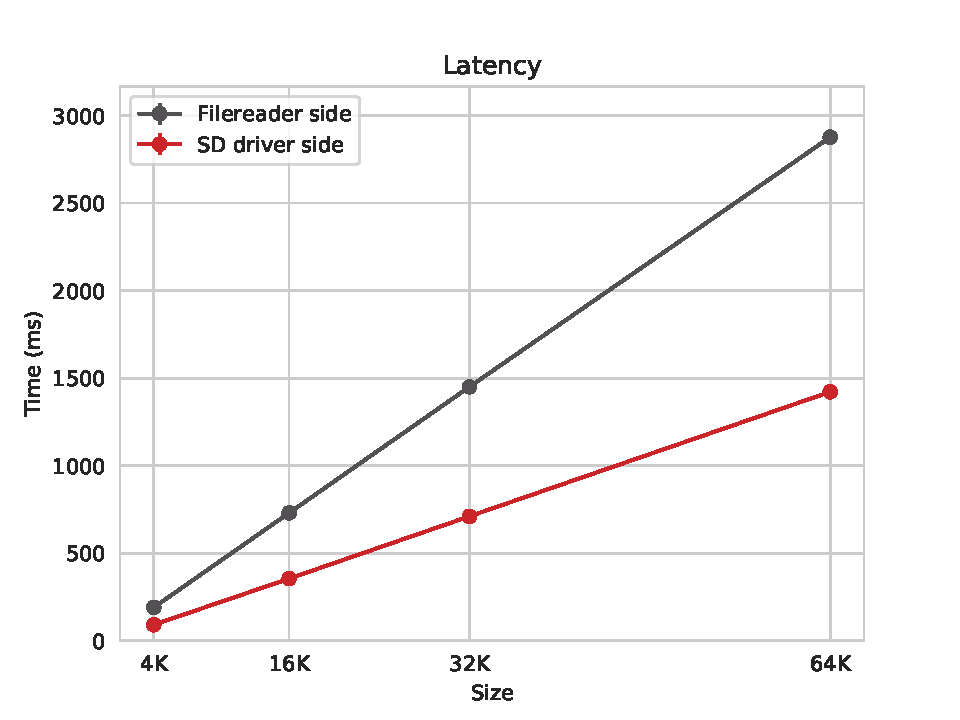
\includegraphics[width=0.7\linewidth]{assets/fs_latency.pdf}
	\caption{Latency difference among user space side and driver side}
	\label{fig:fs_side_diff}
\end{figure}
The growth of both the latencies are linear, meaning that the overhead introduced is constant and related to the amount of data read from the SD.
The parties involved in this process are mainly:
\begin{itemize}
    \item the code to read from the driver
    \item the code responsible to move things from one process (or a core) to another
\end{itemize}
Since the former is capped to the SD card, and works as a baseline for this latency graph, we can assert that the overhead we see in the graph is completely introduced by the URPC, which gets a little bit slower when the amount of data grows.
\paragraph{Last cluster caching}
We will first analyze the performances of reading a long file with and without the last cluster caching.
\begin{figure} [H]
	\centering
	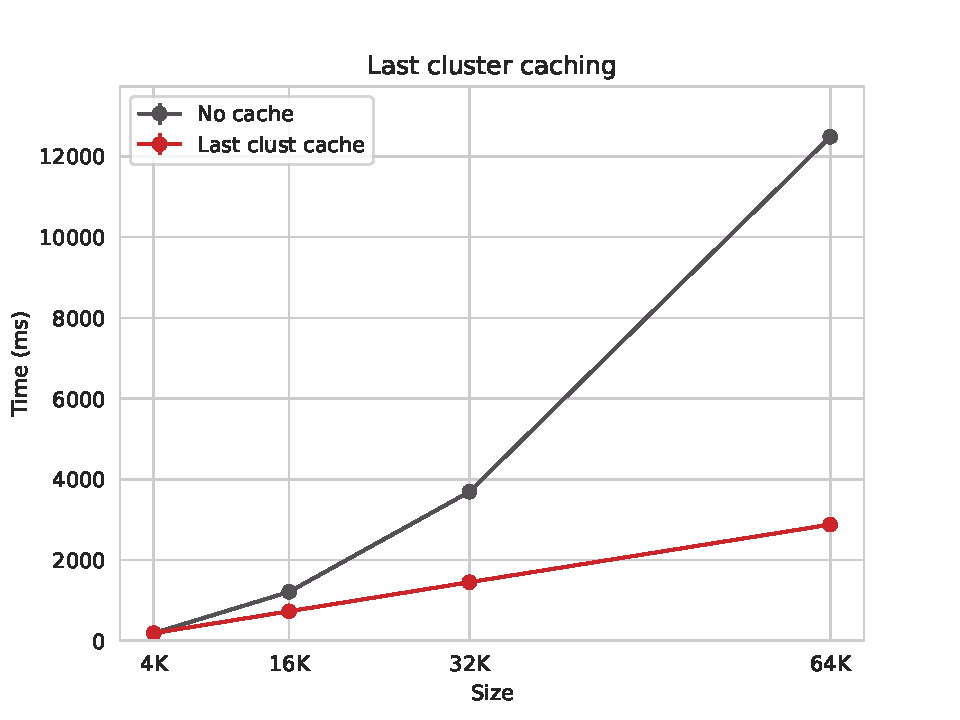
\includegraphics[width=0.7\linewidth]{assets/fs_last_clust.pdf}
	\caption{Caching last cluster vs traversing the chain always}
	\label{fig:fs_last_clust_perf}
\end{figure}
As we can see from the graph, the gain is quite impressive.
The non-linear growth of the case non improved version, is although expected
If we reason about it, the bigger the file, the more the overhead of traversing the clusters chain grows.
So with this improvement, not only we obtained a significant speedup, but most importantly, we avoided an exponential overhead in reading and writing large files.

\paragraph{Filesystem abstraction caching}
Then, we can analyze the improvement introduced by the abstraction of the filesystem.
For this test, we made read some nested directories multiple times with the following commands:
\begin{pandacode}
test_read_dir(MOUNTPOINT "/");
test_read_dir(MOUNTPOINT "/" "white");
test_read_dir(MOUNTPOINT "/" "white" "/"  ".");
test_read_dir(MOUNTPOINT "/" "white" "/" "rabbit" "/" "..");
test_read_dir(MOUNTPOINT "/" "white" "/" "rabbit");
test_read_dir(MOUNTPOINT "/" "white" "/" "rabbit" "/" "."
                                    "/" ".." "/" "." "/" "rabbit");
\end{pandacode} 
The results obtained from the tests are summed up in table \ref{tab:cached_abs}. We can see that we obtained a 2x speedup.
Again, it is quite obvious where the speed up comes from, which is, we are making less request to the driver, since the process is caching the
structure of the system, as long as it not modified.
\begin{table}[H]
\centering
\begin{tabular}{@{}lll@{}}
\toprule
         & Time (ms) & Std (ms) \\ \midrule
No cache & 7651.6    & 108.3    \\
Cached   & 3602.0    & 5.1      \\ \bottomrule
\end{tabular}
\caption{Cached vs Non cached abstraction}
\label{tab:cached_abs}
\end{table}



%\chapter{Application Examples} \label{applications}
%\section{hacks}
%arm-linux-gnueabi-strip armv7/sbin/hello

\chapter{Terminal} \label{cap:term}

\section{Reading from the keyboard}

During \t{init}'s startup, we setup the interrupt handler for the terminal
in the following way:
\begin{pandacode}
volatile uint16_t readterm_idx = 0;
char readterm_buf[READTERM_BUFSIZE];

void handle_uart_getchar_interrupt(void *args) {
	if (readterm_idx == READTERM_BUFSIZE) return;
	sys_getchar(&readterm_buf[readterm_idx++]);
}

int main(void) {
	...
	inthandler_setup_arm(handle_uart_getchar_interrupt, NULL, 106);
	...
}
\end{pandacode}

Basically, init will receive interrupts from the keyboard and store the characters 
typed in a global buffer called \t{readterm\_buf}. This buffer acts as a LIFO, 
and is read through this function:

\begin{pandacode}
char* consume_readterm_buf(int count) {
	while (readterm_idx < count) {
		if (HARDWARE) {
			event_dispatch(get_default_waitset());
		} else {
			sys_getchar(&readterm_buf[readterm_idx++]);
		}
	}
	readterm_idx -= count;
	return &readterm_buf[readterm_idx];
}
\end{pandacode}

\t{HARDWARE} is a boolean variable that indicates if the code is being run on
the Pandaboard or is being virtualized through QEMU. This was necessary because
we didn't have the necessary knowledge with QEMU to make interrupts work, so we
had to settle for a blocking call to \t{sys\_getchar()}.

Processes other than init can read the keyboard through an lmp call to init,
\t{aos\_rpc\_serial\_getchar()} for a single character,
\t{aos\_rpc\_serial\_read()} for a number of characters at the same time.
Also, libc's functions work too (e.g. \t{scanf()}) since we changed the pointer
\t{\_libc\_terminal\_read\_func} to a stub which calls
\t{consume\_readterm\_buf()} if the calling process is init, and
\t{aos\_rpc\_serial\_getchar()} otherwise.


\section{Printing output}

Sending text to the serial as output is done through the syscall
\t{sys\_print()} if the calling process is init; otherwise a call to
\t{aos\_rpc\_serial\_putchar()} or \t{aos\_rpc\_serial\_puts()} will send that
text to init that will then print it through the previous syscall.
As before, libc functions like \t{printf()} work as specified.

\section{Bush - the Barely Usable SHell}

The actual shell is implemented in \t{usr/bush/bush.c}.  It consists of a
simple while loop that scans strings in input and parses them as commands.  The
first word is parsed as the command to run; the rest of the string in input is
sent as argument to the command. There are a set of \emph{builtin} commands
such as \t{echo} and \t{help}; if the provided command does not match any of
the builtins, then the shell will try to find an executable with the same name
in the current folder, and run it.

This is the current list of \emph{builtins}:
\begin{pandacode}
typedef void (*callable)(char*);
typedef struct {
	const char *name;
	callable func;
} builtin;

const builtin builtins[] = {
	 {"blink_leds", blink_leds},
	 {"calculator", calculator},
	 {"cat", cat},
	 {"echo", echo},
	 {"help", help},
	 {"time", time_cmd},
	 {"oncore", oncore},
	 {"run_test", run_test},
	 {"ls", ls},
	 {"cd", cd},
	 {"pwd", pwd},
};
#define builtin_num (sizeof (builtins) / sizeof (builtin))
\end{pandacode}

Notable entries are:
\begin{itemize}
	\item \t{time}:
		Takes another command as argument. Will run said command and on
		successful termination will report the time spent executing that
		command.

	\item \t{blink\_leds}:
		Will blink the two leds of the pandaboard. Takes an integer as 
		argument that represents the number of milliseconds of delay
		of the blinking.

	\item \t{calculator}:
		Starts an interactive, extremely simple calculator that can solve
		queries like \t{5 + 5} or \t{2 * 8}.

	\item \t{run\_test}: 
		Will make init process run a test of the operating system out of our
		testing framework. Takes the type of test as an argument.  Possible
		types of test are: \t{mem}, \t{paging}, \t{proc}, \t{rpc}, \t{cores},
		\t{filesystem}. If no argument is provided, all tests will be run.

	\item \t{oncore}:
		Spawns the given process on the specified core. 
		The syntax of this command is \t{oncore <0|1> <process\_name>}.

	\item \t{ls, cat, pwd}:
		Those commands are the equivalent of the standard UNIX ones and
		let you navigate the filesystem tree.

\end{itemize}

If the provided command does not correspond to one of the builtins, then the multiboot
image is searched for a module with the same name as the command. If that module is
found, than it will be spawned on the same core where the terminal is running.

If no corresponding multiboot module is found, the current folder of the filesystem
is searched for a binary with the same name as the provided command. If a binary is
found, than that binary will be spawned from the SD and run on the same core where
the terminal is running.

\subsection{Extra challenge: Telnet shell}
When a basic implementation of UDP was working, we begun thinking on ways to make
the shell work through a network tunnel.

Since the terminal used only libc functions for dealing with input/output, we had to make
sure that the correct callbacks were set into \t{barrelfish\_libc\_glue\_init}:
\begin{itemize}
	\item \t{\_libc\_terminal\_read\_func}: Function called by all libc's functions like
		\t{scanf}, \t{fgets}, \t{getchar}, etc... 
		This took as argument the buffer in which to read, and 
		the number of characters to read, although many times
		libc requested only one char at the time. If the shell
		was spawned through the network, this callback was mapped to the
		following \t{network\_consume\_buf()}:
		\begin{pandacode}
sock_res * net_msg = NULL;
size_t msg_avail = 0;
size_t msg_curr  = 0;
static size_t network_consume_buf(char * buf, size_t count) {
	size_t cons = 0;
	if (msg_avail == 0)
		network_recv();

	while (cons < count && msg_avail) {
		msg_avail--;
		buf[cons++] = net_msg->buf[msg_curr++];
	}
	return cons;
}
		\end{pandacode}
		where \t{network\_recv()} received a single UDP packet from port 22.
		This function may not be able to satisfy completely the request (in fact, it can
		return up to how many bytes fit into the latest received UDP packet); but since
		it returns the exact number of characters read, it will be called another time
		by the libc, until the required number of characters are read.
	\item \t{\_libc\_terminal\_write\_func}: Function called by all libc's functions like
		\t{printf}, \t{puts}, \t{putchar}, etc... 
		This too took as argument the buffer of characters to write and
		one integer with the number of characters to write. 
		This callback was mapped to the following \t{network\_write()}:
		\begin{pandacode}
static inline size_t network_write(const char *buf, size_t len) {
	sock_res* msg = malloc(len + sizeof(sock_res));
	msg->src = dst; 
	msg->sport = port;
	msg->len = len;

	memcpy(msg->buf, buf, len);
	urpc_write_msg(&sock_urpc, (void**) msg, len + sizeof(sock_res));
}
		\end{pandacode}
		where \t{port} is the port of the client which is connected to the shell.
\end{itemize}

But the above code cannot work without taking care of two particular things before:
\begin{enumerate}
	\item \emph{How does a process (in this case, the shell) know if it was spawned through
		the network?}\\
		The only one who could tell a process that it was spawned through the network 
		was the process' father. However, we had not implemented channel setup of 
		a process with its father.

		Looking for a faster solution, we settled for adding a flag \t{fd}
		inside the dispatcher of a process that the father could set while
		creating it inside \t{spawn\_load\_by\_name()}

	\item \emph{How does the network write function know which port is the client from?}\\
		This was a problem since the usually the port from which the client connected
		was pretty much random, and the function \t{network\_write} had no way of knowing 
		which it was before reading a packet.

		For this reason, if a process is spawned from the network, it will wait for a receiving
		packet before writing anything back into the network, to keep track of the port.
\end{enumerate}

\chapter{Network Stack} \label{cap:nm}
The network stack offers a partial implementation of the IP Protocol Suite, with the notable absence of TCP.
The stack architecture is modular, and it is loosely inspired to FreeBSD \texttt{mbufs} and Linux's \texttt{sk\_buf}.
The ``Network Manager'', \emph{NetMan}, manages all of the network devices and handles the packet queues. NetMan will initialize the network devices, providing them with a callback for packet reception, and maintain a single queue for all the incoming packets.

\begin{figure} [H]
	\centering
	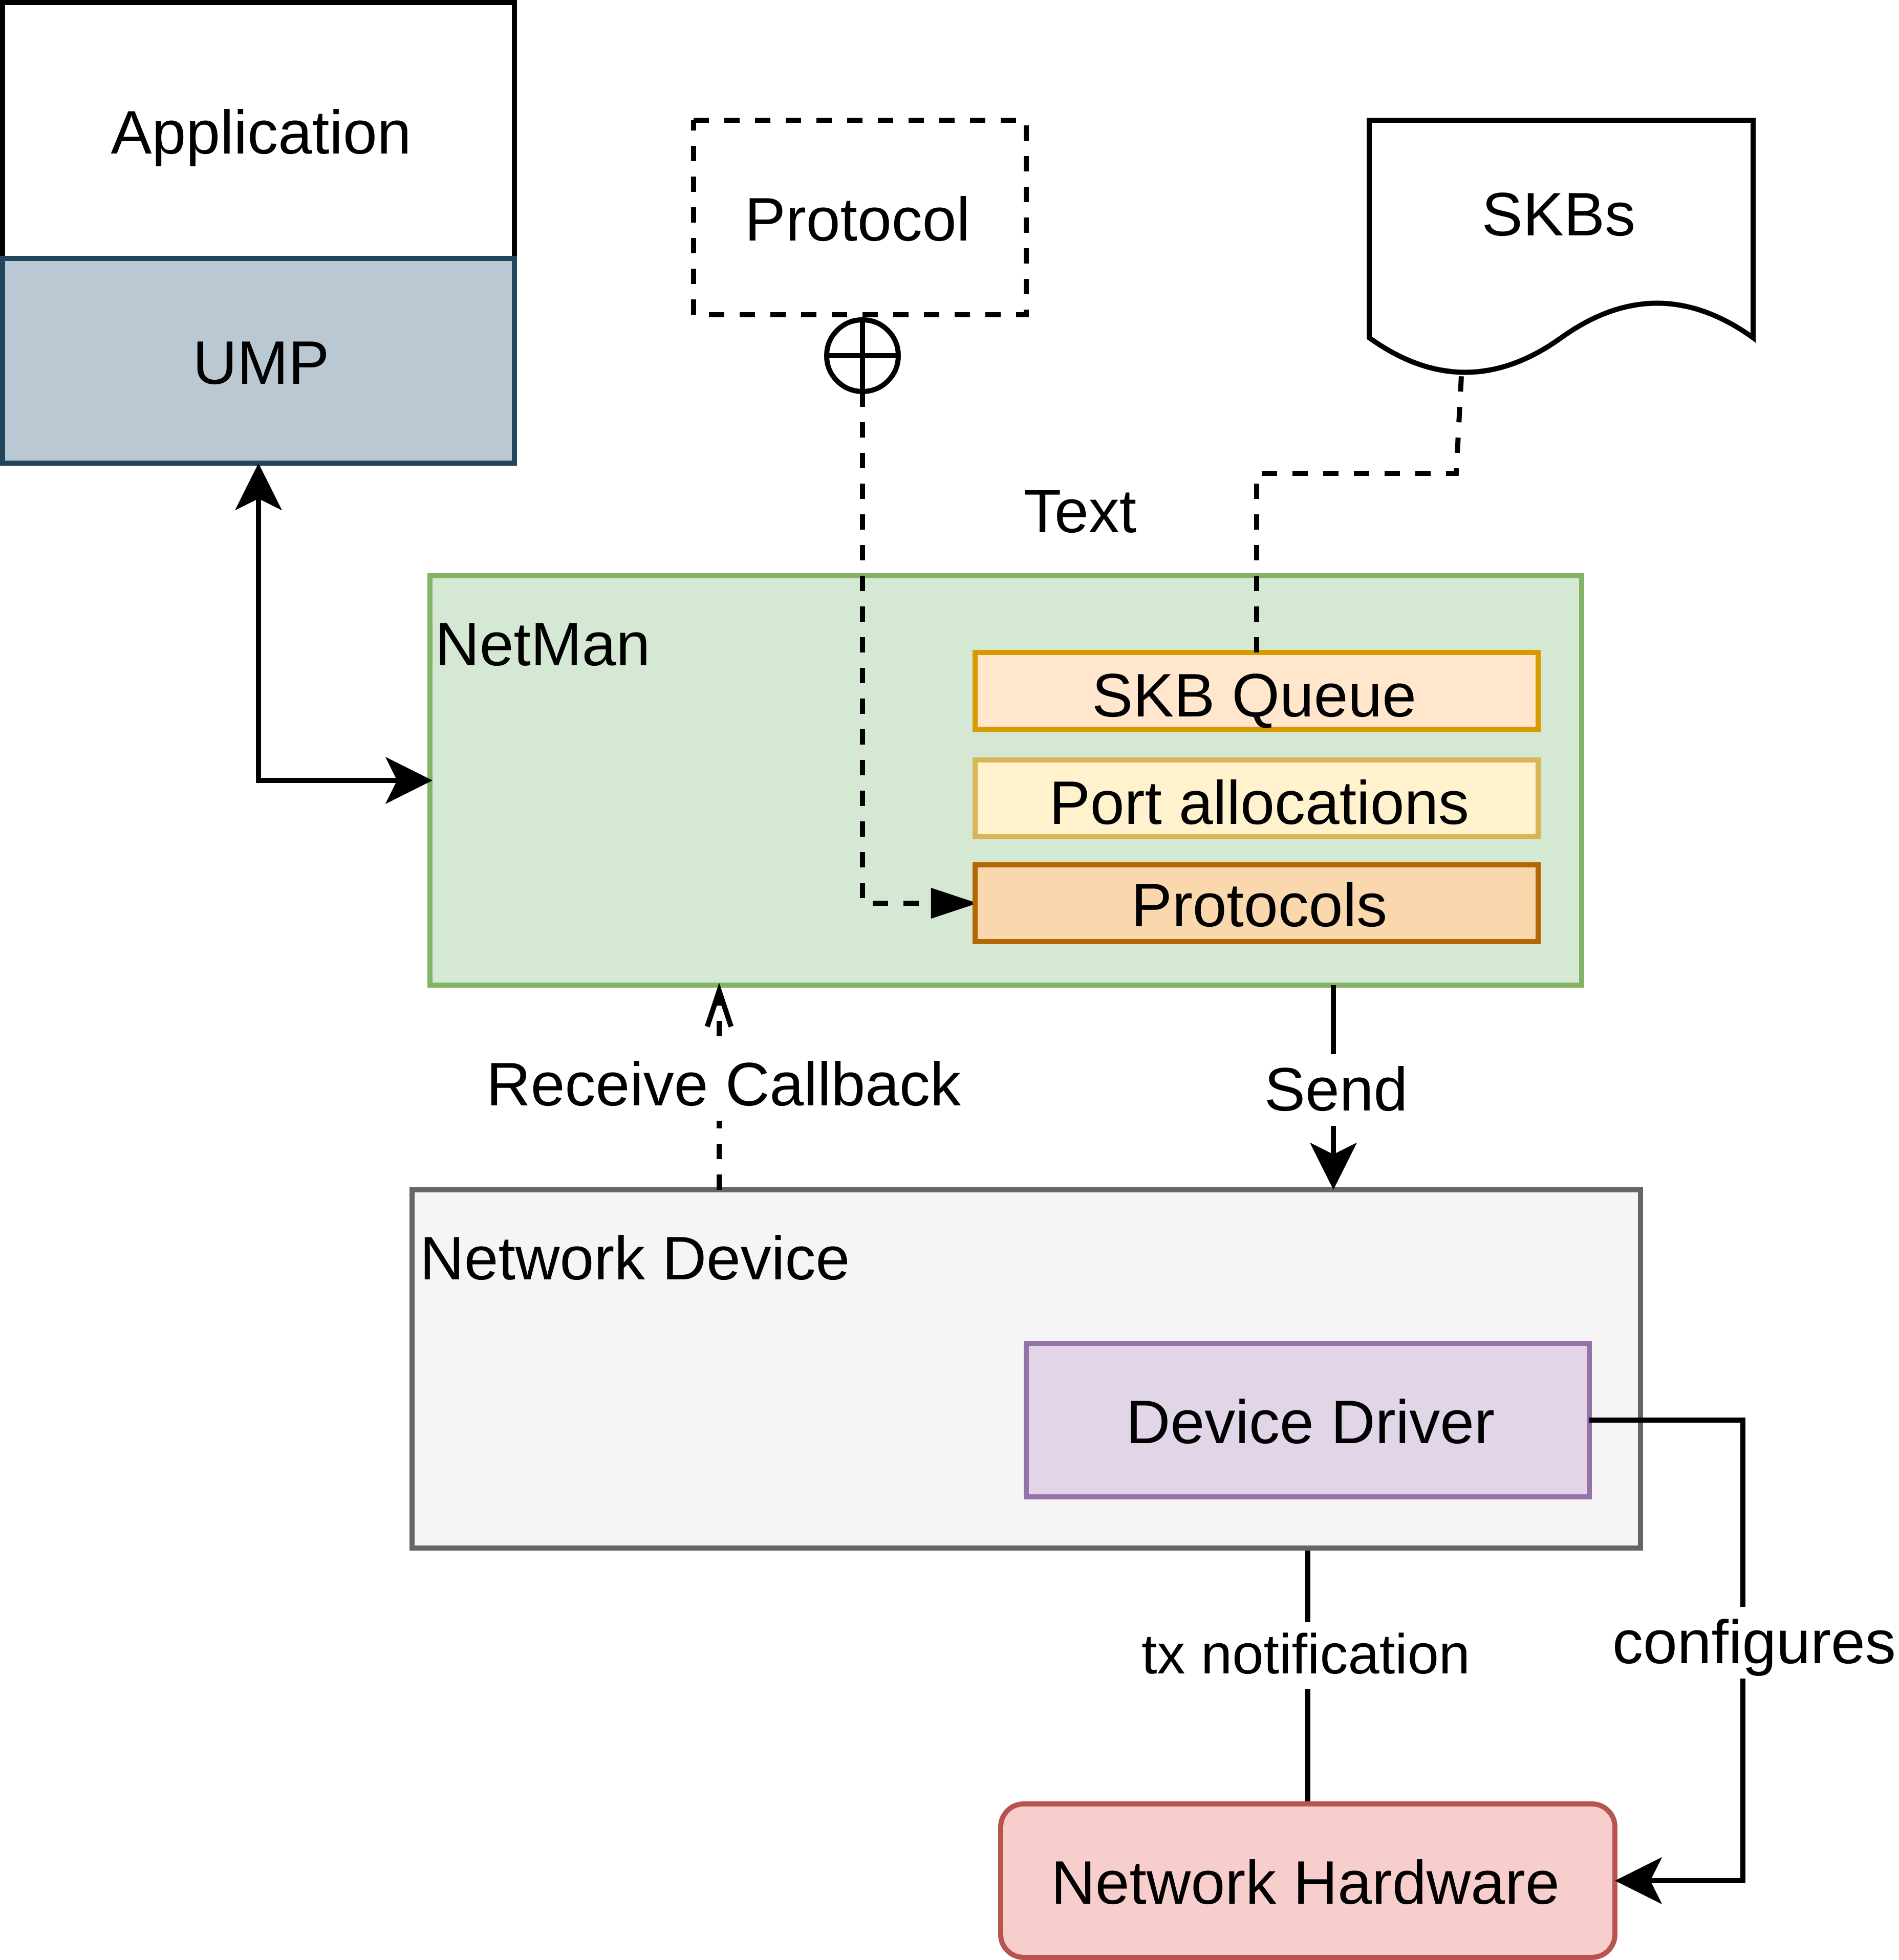
\includegraphics[width=0.7\linewidth]{assets/networkstack}
	\caption{An high level view of the current Network Stack architecture.}
	\label{fig:networkstack}
\end{figure}

Applications interact with NetMan using a socket-like UMP interface. All the incoming and outgoing packages will be passed thought the UMP frame - the received packer queue will be populated by the network devices, while for the outgoing packets the UMP interface will act as a queue.

This design is by far not the most efficient: inside the NetMan, packets are only copied once - from the network device to the socket buffer and vice versa, but for interfacing with client application over the UMP channel, two additional copies - in and out the channel - are required. Alternative designs, like the one found in Nemesis\cite{nemesis}, would probably reduce the number of copies to just one - the network stack would be implemented as an application library, and the shared network service would only need to provide queues and multiplexing.

Trying to implement a Nemesis-like network stack was tempting, but at the end the comparatively easier and more familiar design won, also over fears of running out of time halfway trough the implementation.

The heart of the network stack is the \emph{socket buffer}: a variable-size buffer with generic support for network protocols from mac to application level.

\section{Socket Buffers}
\begin{figure}[H]
	\centering
	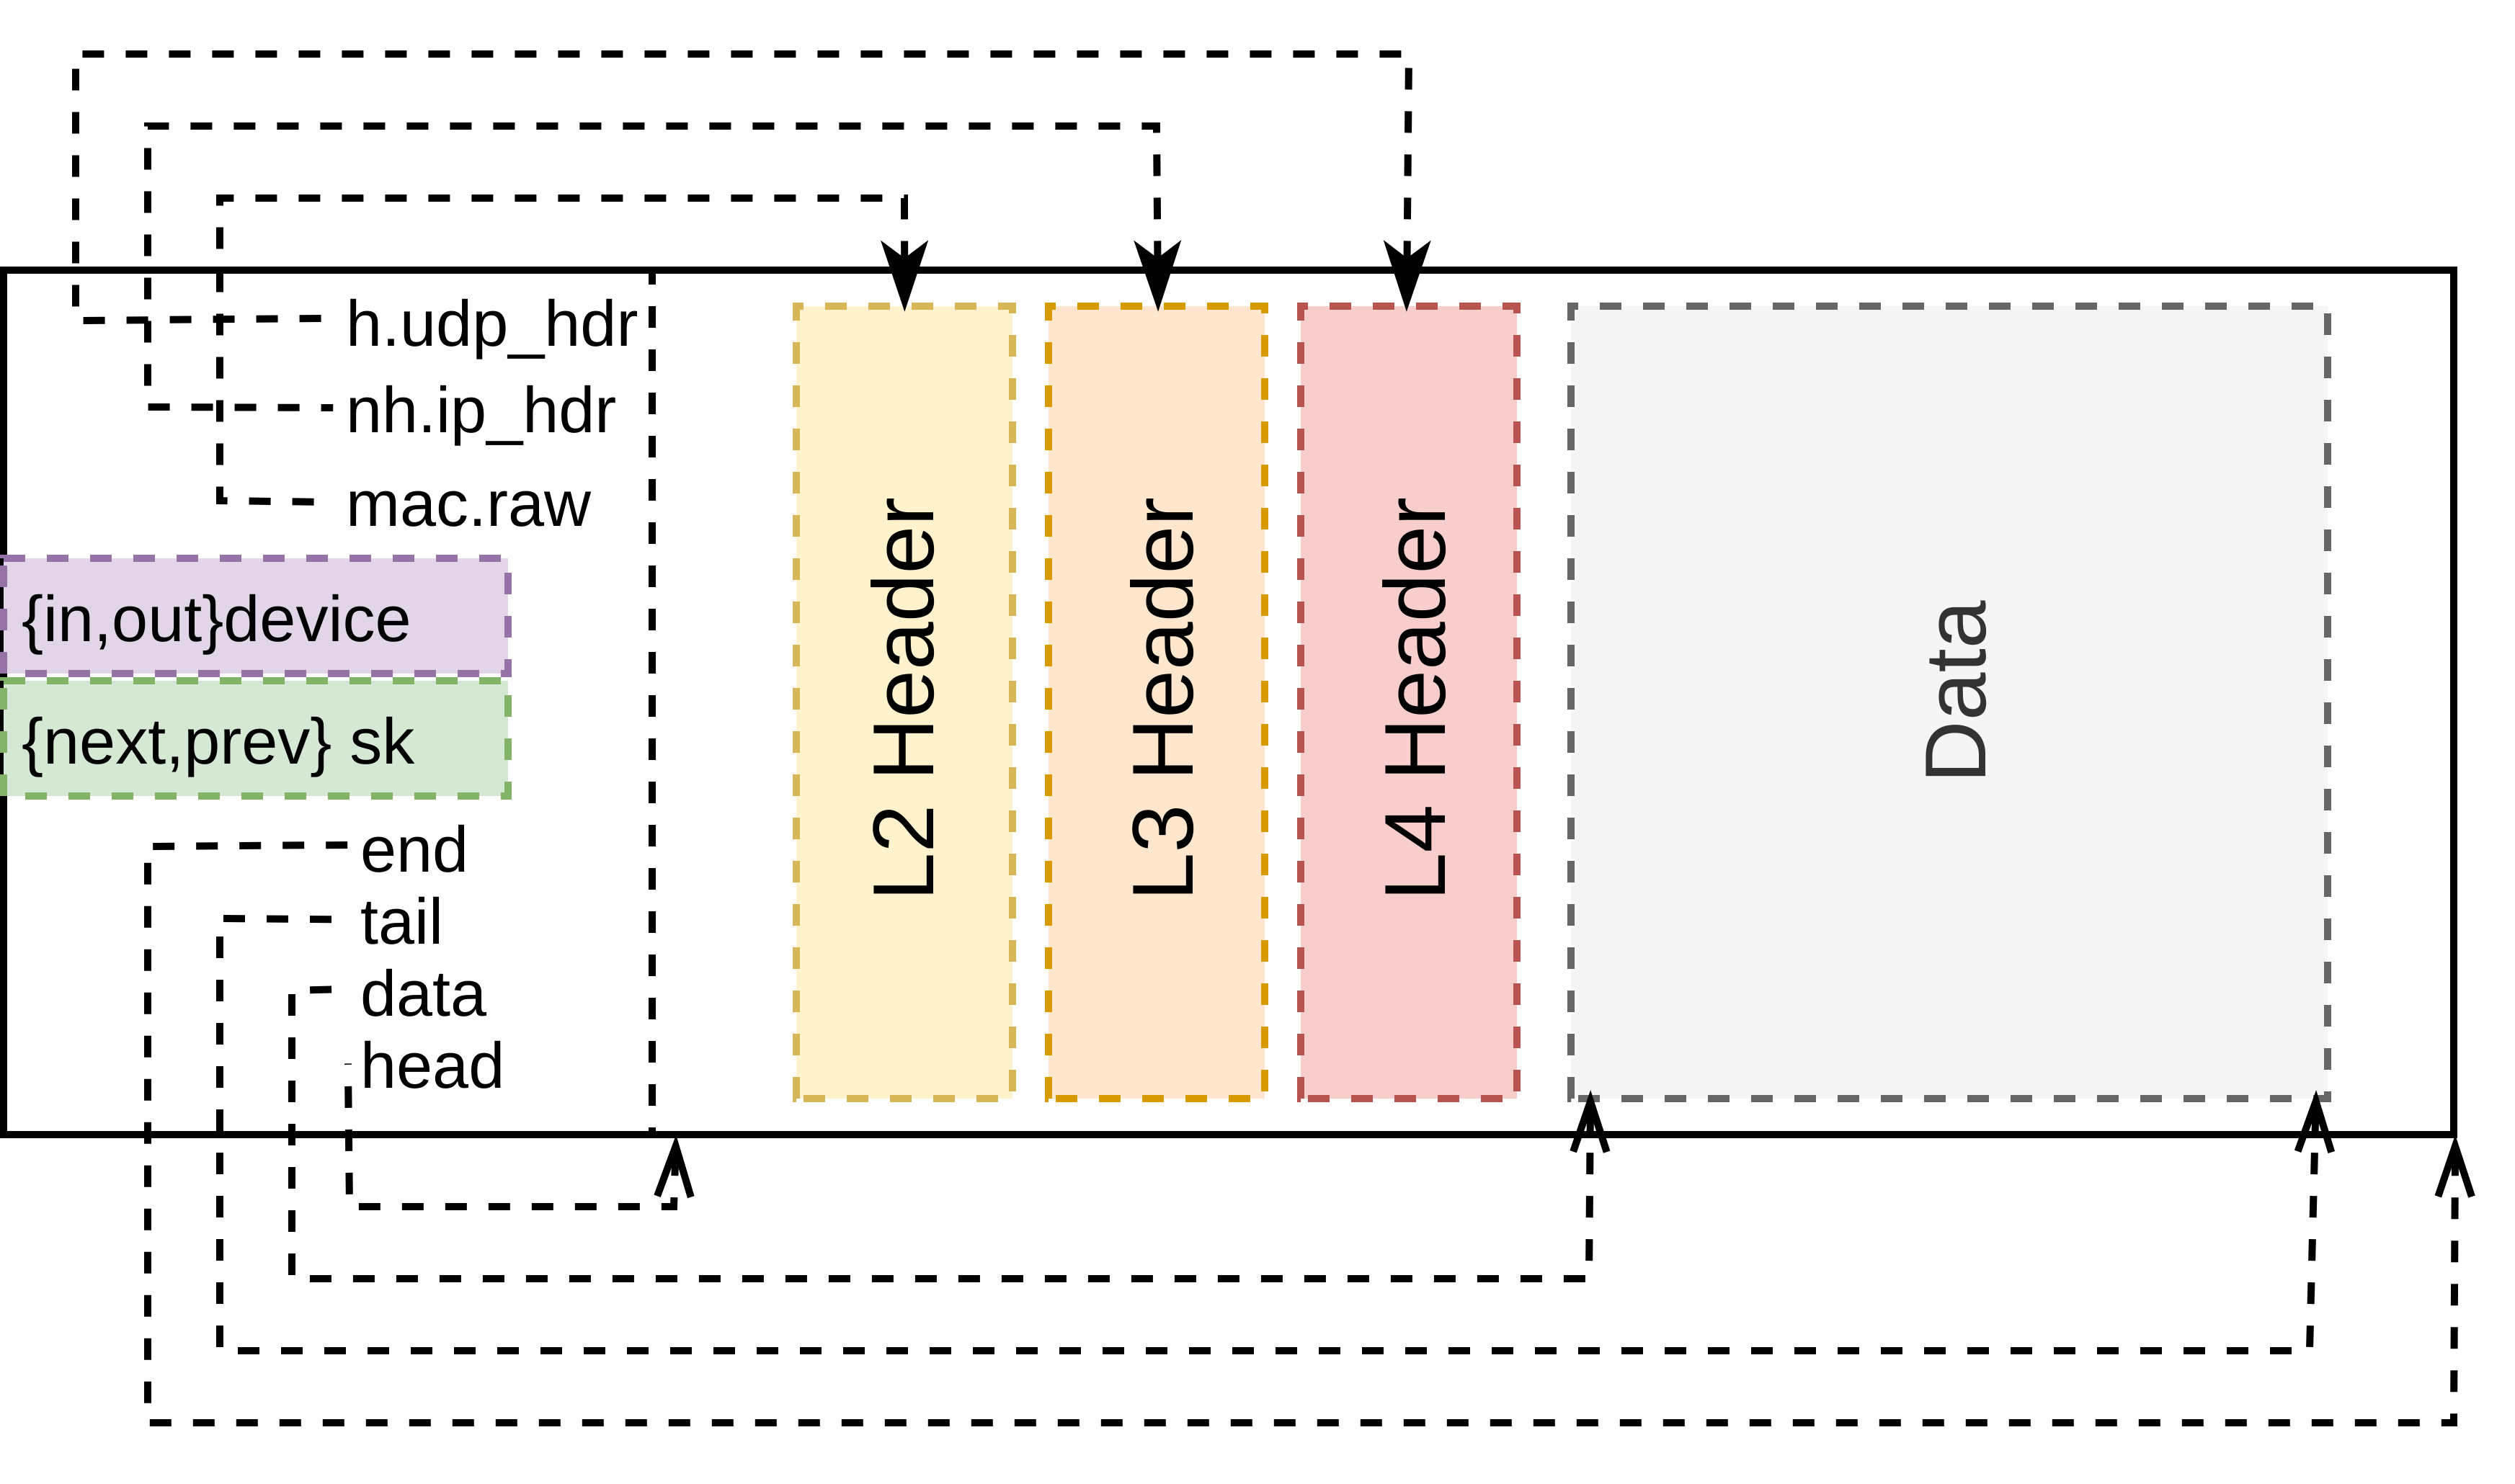
\includegraphics[width=0.7\linewidth]{assets/skbuf}
	\caption{A socket buffer.}
	\label{fig:skbuf}
\end{figure}

All the components of the network stack work with sockets buffers, either producing or consuming them. When an interface produces a packet, it allocates the relative socket buffer, and when the packet is transmitted the relative socket buffer is freed.

The socket buffer data structure is composed of and header and a packet buffer. The header contains meta-information about the type of the packet carried inside the buffer, its current elaboration state and pointers for each ISO/OSI level's protocol header, as well as pointers to raw data start and end inside the buffer.

In its initial state, all the protocol pointers in the socket buffer are uninitialized, the \texttt{head}, \texttt{data} and \texttt{tail} pointers all point to the start of the buffer, \texttt{end} points one byte past the end of the buffer, and the length is zero.

When a packet is received, it is read inside the \t{sk\_buff} buffer: the tail and length values are updated (\t{skb\_put}), the input interface is assigned, and the appropriate headers are initialized and set.

At each level of the network stack, the code responsible for handling a certain protocol will remove the header of the protocol from the front of the buffer adjusting the data pointer and the length (\t{skb\_pull}), initialize the protocol's header, and pass the same \t{sk\_buf} to the next layer, until it receives an application protocol handler that will possibly send the contents to the application layer.

When sending a packet, a new socket buffer is allocated: some space is reserved for the (unknown) lower layers protocols by adjusting the \texttt{data} and  \texttt{tail} pointers (\t{skb\_reserve}), and the packet data is written in the buffer (\t{skb\_put}).

At each level of the network stack, a protocol header will be added, adjusting the data pointer and the length (this time, \t{skb\_put}) and initializing the protocol fields. The socket buffer eventually reaches the L3 (usually IP) layer, where it is routed and scheduled for transmission on a device.

\section{Implemented protocols}
The implementation selectively implements the most important component of UDP and ICMP in the Internet Protocol Suite.

Protocols are currently implemented as header-only libraries, all the functions are inlined for optimization.

\subsection{L3: IP}
Basic IP functionalities are implemented - IP fragmentation and additional header are not supported, but packets are checked for validity when received and correctly built when sent.

The ip library \t{inet.h} provides two functions - \t{ip4\_tx\_handle} and \t{ip4\_rx\_handle}, respectively called on incoming and outgoing socket functions - they check or compute the IP checksum, and prepare the socket buffer for the L4 handlers or for the network devices.

A third function, \t{ip4\_tx\_prefill}, sets up the the various field in the ip header, like destination, port and protocol number. The prefill/handle separation is useful in the common case of packet reflection: if a packet only needs to be re-routed or sent back alike, it is not necessary to change any field in the header with the exception of TTL and checksum, and the handle can be called directly.

\subsection{L3: ICMP}
Even if technically ICMP is L3, it behaves like all the others application layer protocols, since it is wrapped inside an IP header.

\t{ICMP\_rx\_handle} handles, currently, \t{ICMP\_ECHO}, \t{ICMP\_ECHOREPLY} and \t{ICMP\_DEST\_UNREACH} icmp types.

\t{icmp\_echo\_req} allows the caller to send an echo request.

\subsection{A fastpath: ICMP echo reply}

\subsection{L4: UDP}

\section{Network Device Abstraction}
The network devices allows the network manager to abstract over the hardware. NetMan will call the device's allocation and initialization functions, register the device and start a thread on their event loop.
The devices also offer a teardown function, as well as 

Registered devices are assigned a static IP at runtime, and are for now kept in a doubly linked list.


\subsection{SLIP Netdev}
The slip network device implements an rfc1055-compliant Serial Line Internet Protocol interface.

This interface was not separated from the serial driver due to performance concerns.

By default, the slip is assigned the IP address block 10.0.0.0/8, and the IP 10.0.0.1.

\subsubsection{The serial driver}
A serial driver was already provided in \t{user\_serial}. 

A simple (and quite fast) serial driver callback is called by the driver and passes each read character directly to the SLIP deserialization routines.

When a packet is completed, the NetMan callback is invoked with the corresponding socket buffer.

\subsection{LO Netdev}
The loopback (\textbf{lo}) network device is a very simple device that loops packet back into the network stack.

Following the RFC8190, the lo device is assigned the address block 127.0.0.0/8.


\subsection{Routing}
Given the extremely reduced scope of the project, a simple first-subprefix match algorithm for determining packet's output device was deemed sufficient.

\begin{figure} [H]
\begin{pandacode}
static bool prefix_match(in_addr_t net, in_addr_t ip, in_addr_t mask) 
	if ((net & mask) == (ip & mask))
		return true;
	else
		return false;

static inline netdev * ip_route(in_addr_t addr, sopt * opt)
	dlinked_node_t* node = netman->netdevs.head;
	while (node)
		netdev * nd = (netdev *) node;
		if (prefix_match(nd->p.ip, addr, nd->p.mask))
			return nd;
		else 
			node = node->next;
	return opt->default_netdev;
\end{pandacode}
\caption{A (stub) routing algorithm - the interface was programmed to support extension to a more complete routing API}
\end{figure}

A complete network stack would implement the standard longest subprefix match, and a full routing abstraction - here only approximated by input and output devices.

\section{User API}
Netman offers a UMP interface: it publishes an \textit{nm} service, and keeps track of the frames of all the subscribers.

As soon as a frame with the subscriber is bound, Netman spawns a new thread that will handle request to and from that particular frame. The first message is equivalent to a \texttt{bind()} call: the application communicates to Netman the protocol and (eventually) the port it desires to listen on.

\begin{figure} [H]
\begin{pandacode}
	typedef struct sock_req {
		uint32_t magic;
		enum sock_req_t proto;
		uint16_t sport;
		uint16_t dport;
		in_addr_t dst;
    in_addr_t src;
	} sock_req;
\end{pandacode}
\caption{The \texttt{sock\_req} structure, used to request a socket bind}
\end{figure}

After the \texttt{sock\_req} message, every message on the frame will be wrapped in a \texttt{sock\_res} structure. Specifying src and srcport when writing a message in the frame the application can control the destination address and port of the packet, in a similar fashion to the \texttt{sendto} posix call; reading the same fields will report the source address and port of the received message, like in \texttt{recvfrom}.

\begin{figure} [H]
\begin{pandacode}
typedef struct sock_res {
	in_addr_t src;
	uint16_t sport;
	uint16_t len;
	uint16_t seq;
	uint16_t zeros;
	unsigned char buf[];
} __attribute__((packed)) sock_res;
\end{pandacode}
\caption{The \texttt{sock\_req} structure, used to receive and send messages}
\end{figure}

Implementing a full-fledged Berkeley Socket API was not feasible due to time constraints. 

\section{Applications using the network}
\subsection{Terminal}
The terminal is using the network for I/O. File descriptors were not ready at the time of integration, therefore the networks was added in a to say the least strange way: in the libc gluing code, if a certain parameter is set in the dispatcher, the application will bind on a port and use udp input and output on that port as stdin and stdout.

This approach is not flexible, not portable, not maintainable - it was literally the fastest hack we could think of.

\subsection{Echo server}
The echo server implements RFC 862. It binds on port 7, and replies to all the messages it receives with a message carrying the same content.

The echo server is implemented as a standalone dispatcher and accesses the network via the UMP interface: an implementation inside the network manager itself would have been faster - the UMP requires additional 2 copies of the packet, in and out of the UMP frame - but would not have reflected the performance of a normal network application.

\subsection{Ping}
The ping utility produces ICMP ECHO requests. At the current stage it is quite barebone - it does not feature the classic RTT calculation.

RFC1122-compliant echo replies are implemented inside the network manager.

\begin{figure}
	\centering
	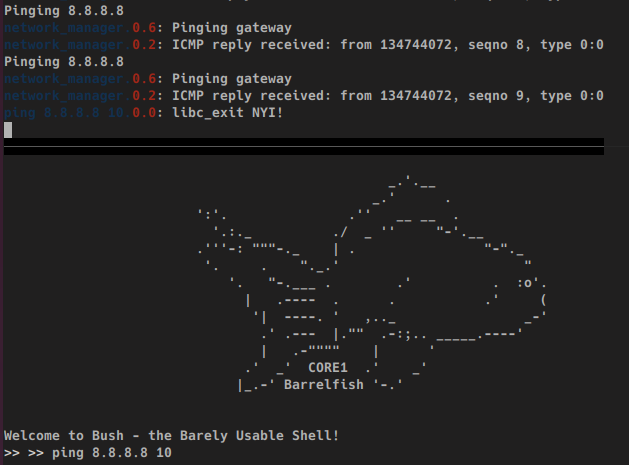
\includegraphics[width=0.7\linewidth]{assets/net_term_ping}
	\caption{A remote shell over netcat (bottom) and picocom (top) showcasing a ping to Google's DNS Resover (8.8.8.8).}
	\label{fig:nettermping}
\end{figure}

\bibliographystyle{unsrt}
\bibliography{report}

\appendix 
\addcontentsline{toc}{chapter}{APPENDICES}

%\chapter{API Reference}

\chapter{Experiences}
Nightmares:
\begin{itemize}
	\item having to press the reset button on the Pandaboad
	\item debugging the (currently unsolved) MMU/kernel paging inconsistency issue
	\item since we didn't write an interrupt handler, Chandu Thekkath won't trust us with his life
\end{itemize}

Dream-like:
\begin{itemize}
	\item developing on qemu - we used the a15ve\_4 emulated machine exclusively, until the individual projects forced us to actually use the boards.
	\item playing with the leds - initialization is boring, but writing low-level drivers that interface
	\item writing a network stack
\end{itemize}

\chapter{APIs}
The usage examples and the description of the main programming interfaces we provide is covered in the corresponding chapters.

For the not explicitly documented interfaces, it is possible to find comments and self-documenting code inside our gitlab repository.

\end{document}


